\documentclass{article}

% ============================================
% arXiv preprint style (shared with companion paper)
% ============================================

\usepackage{arxiv}

% Encoding
\usepackage[utf8]{inputenc}

% Math
\usepackage{amsmath,amssymb,amsthm}
\usepackage{mathtools}

% Tables and figures
\usepackage{graphicx}
\usepackage{booktabs}
\usepackage{array}
\usepackage{float}

% Lists
\usepackage[inline]{enumitem}

% Colors
\usepackage{xcolor}
\usepackage{colortbl}

% URLs and citations
\usepackage{url}
\usepackage{natbib}
\usepackage[colorlinks=true,linkcolor=blue!60!black,citecolor=blue!50!black,urlcolor=blue!50!black]{hyperref}
\usepackage{orcidlink}

% Code listings
\usepackage{listings}
\usepackage{tikz}
\usetikzlibrary{shapes.geometric, arrows.meta, positioning, calc, fit, backgrounds, shadows.blur, decorations.pathreplacing}
\usepackage{pgfplots}
\pgfplotsset{compat=1.17}
\usepgfplotslibrary{fillbetween}
\usepackage{tcolorbox}
\tcbuselibrary{skins,breakable}

% Clarification box for preemptive counterarguments
\newtcolorbox{clarification}[1][]{
    enhanced,
    breakable,
    colback=blue!3,
    colframe=blue!40!black,
    coltitle=white,
    fonttitle=\bfseries,
    title=Clarification,
    left=3pt,
    right=3pt,
    top=2pt,
    bottom=2pt,
    boxrule=0.5pt,
    arc=2pt,
    #1
}

\usepackage{subcaption}
\usepackage{capt-of}

% JSON styling for schema listings
\lstdefinelanguage{json}{
    basicstyle=\ttfamily\scriptsize,
    showstringspaces=false,
    breaklines=true,
    frame=single,
    backgroundcolor=\color{gray!3},
    rulecolor=\color{gray!40},
    framesep=3pt,
    xleftmargin=3pt,
    xrightmargin=3pt,
    literate=
      *{:}{{{\color{gray!70}:}}}{1}
       {,}{{{\color{gray!70},}}}{1}
       {\{}{{{\color{codecolor}\{}}}{1}
       {\}}{{{\color{codecolor}\}}}}{1}
       {[}{{{\color{auditcolor}[}}}{1}
       {]}{{{\color{auditcolor}]}}}{1}
       {"}{{{\color{governcolor}"}}}{1},
    morestring=[b]",
    stringstyle=\color{blue!60!black},
}

% Define colors for test names
\definecolor{exitcolor}{HTML}{06B6D4}
\definecolor{codecolor}{HTML}{3B82F6}
\definecolor{auditcolor}{HTML}{A855F7}
\definecolor{governcolor}{HTML}{F59E0B}
\definecolor{forkcolor}{HTML}{F472B6}

% Theorem environments
\newtheorem{definition}{Definition}[section]
\newtheorem{proposition}{Proposition}[section]
\newtheorem{claim}{Claim}[section]
\newtheorem{theorem}{Theorem}[section]
\newtheorem{condition}{Condition}[section]
\newtheorem{corollary}{Corollary}[section]
\newtheorem{remark}{Remark}[section]
\newtheorem{principle}{Principle}[section]

% (arxiv.sty provides \keywords{...})

% cleveref for navigable cross-references
\usepackage{cleveref}

% ============================================
% Title and Author
% ============================================

\title{Corrigibility as a Structural Precondition for Digital Public Infrastructure: A Cybernetic Framework\thanks{SSRN: \href{https://doi.org/10.2139/ssrn.6059075}{doi.org/10.2139/ssrn.6059075}}}

\author{
  Anivar A Aravind~\orcidlink{0009-0009-8995-0005} \\
  Independent Researcher\\
  Bengaluru, India \\
  \texttt{ping@anivar.net}
}

\date{April 2026 \\ {\small Revised: 10 July 2026}}

\hypersetup{
  pdftitle={Corrigibility as a Structural Precondition for Digital Public Infrastructure: A Cybernetic Framework},
  pdfauthor={Anivar A Aravind},
  pdfsubject={Structural corrigibility for digital public infrastructure: cybernetic framework, control-theoretic formalization, five-test architecture (EXIT, CODE, AUDIT, GOVERN, FORK), and empirical assessment of national-scale deployments. SSRN DOI: 10.2139/ssrn.6059075.},
  pdfkeywords={corrigibility, digital public infrastructure, DPI, cybernetics, requisite variety, feedback control, commons governance, free software, infrastructure accountability, non-domination, India Stack, Aadhaar, UPI},
  pdfproducer={pdfTeX},
  pdfcreator={LaTeX with hyperref}
}

\begin{document}

\maketitle

\begin{abstract}
Digital Public Infrastructure is evaluated using aspirational criteria: interoperability, inclusion, openness, scale. These criteria do not establish whether systemic errors can be corrected by affected participants. This paper defines corrigibility as the minimal structural precondition for reversible public infrastructure. Five jointly necessary conditions form a closed corrective loop: EXIT, CODE, AUDIT, GOVERN, FORK. Failure of any condition opens the loop, rendering correction discretionary. Using control-topology mapping grounded in Ashby's Law of Requisite Variety, the paper formalizes corrigibility as an architectural property: partial compliance is structurally equivalent to open-loop operation. Applied analysis demonstrates discriminative power against existing infrastructures. The five conditions are stated as an invariant of the infrastructure rather than of its implementation. A companion paper carries the same invariant to learned and agentic systems, where only the verification machinery changes. Corrigibility does not guarantee fairness. It guarantees reversibility.
\end{abstract}

\keywords{Corrigibility \and Digital Public Infrastructure \and Cybernetics \and Feedback Control \and Requisite Variety \and Infrastructure Accountability \and India Stack}

\section*{Executive Summary}

Can the system be corrected when it goes wrong? The criteria by which Digital Public Infrastructure (DPI) is currently evaluated --- openness, interoperability, inclusion, scale --- do not answer that question.

\textbf{Corrigibility} is the structural ability of affected participants to detect, contest, and override systemic error. Without this property, digital infrastructure operates in open-loop: errors may be acknowledged, but correction remains discretionary.

Five architectural constraints are required for corrigibility:

\begin{enumerate}[noitemsep]
    \item Reversible participation (\textbf{EXIT})
    \item Inspectable logic (\textbf{CODE})
    \item Independent verifiability (\textbf{AUDIT})
    \item Binding participatory constraint (\textbf{GOVERN})
    \item Independent reproducibility (\textbf{FORK})
\end{enumerate}

These constraints operate across observability, participation, constraint, and replacement layers. The absence of any one constraint creates structural asymmetry. The framework provides testable criteria for evaluating real-world DPI systems.

\paragraph{How to Read This Paper.} The argument proceeds in three parts: public systems require bounded error propagation (the invariant); five conditions close the corrective loop (the architecture); these conditions discriminate between real systems (the evaluation). Case studies illustrate discriminative power, not exhaustive institutional assessment.

\section{Introduction}

Digital Public Infrastructure is not merely a collection of software stacks; it is the encoding of political arrangements into technical artifacts \citep{winner1980}. Access to essential survival services (food distribution, banking, healthcare, mobility) is increasingly mediated through these systems. Because these systems apply fixed rules to the infinite variety of human life, they will inevitably misclassify, exclude, or fail specific users. This is not a malfunction; it is a mathematical certainty when finite rule sets encounter human diversity.

The critical question for a digital polity is not whether errors occur, but whether the architecture permits those affected to \textbf{detect, correct, and reverse} them before harm becomes permanent.

Current policy discourse defines DPI through aspirational language. The G20 New Delhi Declaration (2023) and the UN/UNDP framework \citep{undp} describe systems that ``should be secure'' or ``can be built on open standards.'' These definitions exclude almost nothing. They articulate intent, not condition. Under such broad definitions, a system that traps users in a coercive loop can be labeled ``public infrastructure'' simply because it operates at scale.

This paper defines corrigibility not as a moral preference, but as a structural property essential for stability. The central argument is that \textbf{unverifiable constraint is structurally indistinguishable from absolute operator control.} Therefore, public legitimacy requires more than policy assertions; it requires a cryptographic chain of custody and a verifiable capacity for correction. The normative grounding for this structural definition --- non-domination as the criterion for legitimate public infrastructure --- is developed at the opening of Section~\ref{sec:theory}.

\paragraph{Contributions.} This paper formalizes the structural preconditions for public digital infrastructure, transitioning the discourse from normative aspirations to falsifiable engineering constraints. Specifically, the contributions are threefold:
\begin{enumerate}[noitemsep]
    \item \textbf{A Synthesis of Corrigibility}: This framework distills principles from cybernetics, commons governance, and free software into five verifiable structural tests (EXIT, CODE, AUDIT, GOVERN, FORK).
    \item \textbf{Control-Theoretic Formalization}: A control-theoretic structural model (Appendix~\ref{appendix:proofs}) shows that partial compliance with these tests is structurally equivalent to open-loop operation.
    \item \textbf{Empirical Vulnerability Assessment}: The framework evaluates major national infrastructures (e.g., Aadhaar, UPI), formalizing the resource barriers to structural accountability.
\end{enumerate}

\paragraph{Paper Structure.} Section~\ref{sec:problem} diagnoses why current DPI definitions fail. Section~\ref{sec:theory} establishes the theoretical foundations from cybernetics, commons governance, and free software. Section~\ref{sec:tests} derives the five structural tests. Section~\ref{sec:diagnosis} immediately grounds these tests in empirical evaluation of existing infrastructure, establishing concrete stakes before proceeding to dynamics. Section~\ref{sec:political-economy} analyzes the political economy of incorrigibility: temporal dynamics, correction velocity, essential services, and the sovereignty--scale--neutrality tension. Section~\ref{sec:discussion} addresses methodological foundations and implementation pathways. The appendices formalize the control-theoretic model and provide machine-readable schemas for automated assessment. A glossary of key terms appears in Appendix~\ref{appendix:glossary}.

\subsection{Corrigibility: Minimal Structural Definition}
\label{subsec:minimal-definition}

Corrigibility is the property of a system in which affected participants can detect, contest, and structurally override systemic error. It is not equivalent to transparency, accountability, openness, or auditability in isolation. A system may publish documentation, provide APIs, or maintain oversight boards and yet remain structurally incorrigible if participants lack binding corrective leverage.

Formally, a digital public infrastructure is structurally corrigible if and only if it satisfies five jointly necessary conditions --- sufficient only in the narrow sense of structural access to correction --- that together close the feedback loop between system behavior and participant correction. These conditions operate across distinct control layers: observability, participation, constraint, and replacement. The failure of any one condition converts the system into an open-loop structure in which error may accumulate without guaranteed structural correction.

The remainder of this paper defines these conditions and demonstrates their necessity.

\paragraph{Verification Tiers.} Corrigibility can be assessed at three operational tiers: (1) \textit{Presence}: laws, bodies, and policies exist on paper; (2) \textit{Behavior}: controls execute under stress, audits produce consequences; (3) \textit{Proof}: trust is continuously testable, authority is scoped and revocable, claims are machine-verifiable, failures are bounded. Most DPI deployments satisfy Presence. Few reach Behavior. Almost none achieve Proof. The five conditions define what must be verified. The tiers define how rigorously.

\section{The Problem: Definitions Without Structure}
\label{sec:problem}

The accepted definitions of Digital Public Infrastructure share a common defect: they describe desired outcomes without specifying the architectural preconditions required to achieve them. This section dissects the authoritative definitions to demonstrate their structural inadequacy.

\subsection{The Definitional Landscape}

The G20 New Delhi Leaders' Declaration (2023) established the international consensus:

\begin{quote}
``a set of shared digital systems that should be secure and interoperable, and can be built on open standards and specifications to deliver and provide equitable access to public and/or private services at societal scale'' \citep{g20}.
\end{quote}

The UNDP framework \citep{undp} elaborates:

\begin{quote}
``DPI refers to digital solutions that enable basic functions essential for public and private service delivery, including digital identity, payments, and data exchange. These solutions can be built as open-source, with open standards and specifications, and should incorporate principles of inclusion, security, and privacy by design.''
\end{quote}

The World Bank's identification principles add:

\begin{quote}
``[Identity systems should be] robust, inclusive and accountable...responsive to the needs of various users and enrollment contexts...designed to allow for federation, interoperability, and data portability'' \citep{worldbank2021id4d}.
\end{quote}

\subsection{Anatomizing the Aspirations}

These definitions deploy a consistent vocabulary: \textit{secure}, \textit{interoperable}, \textit{open}, \textit{inclusive}, \textit{accountable}. Examined structurally, each term collapses under scrutiny.

\paragraph{``Secure.''}  Secure for whom? A system can be cryptographically robust against external attackers while remaining structurally impervious to those it governs. The CIDR (Central Identities Data Repository) in Aadhaar is ``secure'' in the sense that it resists breaches. It is not secure in the sense that citizens can verify its operation or contest its determinations. Security without accountability is a fortified monopoly.

\paragraph{``Interoperable.''}  Interoperable with what? A system that speaks standard protocols to upstream services while maintaining proprietary control over downstream users achieves interoperability for operators, not subjects. UPI's API specifications are interoperable; citizens cannot interoperate with NPCI's switching logic. The interface is public; the machine is private.

\paragraph{``Open Standards.''}  Open standards are not open execution. As Simon Phipps of Sun Microsystems observed, ``FOSS serves as the canary in the coalmine for the word `open'. Standards are truly open when they can be implemented without fear as free software in an open source community'' \citep{phipps2007}. PDF is an open ISO standard; Adobe Acrobat's execution of it is proprietary. A system can speak a public language while its internal logic remains invisible. Similarly, a payment rail can implement open APIs while its routing algorithms, fee structures, and dispute resolution mechanisms remain black boxes. Publishing a specification does not make a system inspectable. The critical question for any ``open standard'' claim is: \textit{which open standard?} If the specification URL cannot be shared publicly, or if the standard cannot be implemented in free software without legal encumbrance, the openness is performative.

\paragraph{``Inclusive.''}  Inclusive under what conditions? A system that enrolls everyone achieves enrollment inclusivity. But enrollment is the beginning, not the end. A system that enrolls everyone while providing no mechanism for contestation or exit achieves inclusive capture. The question is not ``Can everyone get in?'' but ``Can anyone get out?'' Mandatory enrollment with no exit is not inclusion; it is mandatory lock-in.

\paragraph{``Accountable.''}  Accountable to whom, through what mechanism, with what enforcement? The definitions invoke accountability as an adjective, not a structure. They specify no verification procedure, no audit right, no correction channel. Accountability without mechanism is rhetoric.

\subsection{The Four Structural Gaps}

The definitional inadequacy manifests as four distinct capture vectors:

\textbf{First, Open Standards are not Open Execution.} A proprietary system can speak a standard language while remaining entirely opaque in its internal logic. (Addressed by the \textbf{CODE} test, Section~\ref{sec:tests}.)

\textbf{Second, Legal Frameworks do not guarantee Technical Rights.} A system that requires a court order to correct a database error effectively denies correction to the majority of its users. Legal remedy operates on bureaucratic timescales that cannot match infrastructure execution speed. (Addressed by the correction velocity inequality, Section~\ref{sec:dynamics}.)

\textbf{Third, Aspiration is not Compliance.} Definitions that rely on what a system ``can'' do or ``should'' be offer no resistance to authoritarian drift. Modal language creates no enforceable constraint. Every term in the G20 definition is advisory (``should be secure,'' ``can be built on open standards''). Advisory language excludes nothing. (Addressed by the \textbf{GOVERN} test, Section~\ref{sec:tests}.)

\textbf{Fourth, Scale is not Accountability.} A system that serves a billion users achieves universality, but universal deployment does not confer public legitimacy. Population-scale operation may simply mean population-scale capture. The ``public'' in such definitions refers to the number of subjects, not the structure of control. (Addressed by the essential services problem, Section~\ref{subsec:essential}.)

\subsection{Structural Theater and Open-Washing}
\label{subsec:openwashing-intro}

The absence of structural criteria enables what we term \textbf{Open-washing}: the invocation of openness, interoperability, or digital sovereignty as reputational signals without satisfying reproducibility or governance conditions.

This is not a theoretical concern. Mozilla warned in 2017 that Aadhaar's claims of openness were misleading: ``The development was not open, the source code is not open'' \citep{mozilla2017}. In 2020, Mozilla and the Internet Society cautioned that India's National Open Digital Ecosystems (NODE) framework risked institutionalizing open-washing by leaving ``the definition of `open' vague and at the complete discretion of individual implementers,'' enabling ``closed ecosystems that are only open in appearance while being closed in practice'' \citep{mozilla2020}.

In the absence of EXIT, CODE, AUDIT, GOVERN, and FORK guarantees, claims of openness are merely descriptive properties of implementation rather than enforceable constraints on power. A system may publish APIs, release partial source code, or adopt open standards while remaining structurally incorrigible.

Open-washing therefore constitutes a category error: conflating technical transparency with structural accountability. The corrigibility framework distinguishes \textit{symbolic openness} from \textit{constitutional openness} by requiring that affected participants retain binding pathways for contestation and reproduction.

\subsection{The Definitional Thesis}

Without hard structural requirements, ``Public'' becomes a mere descriptor of scale rather than a mode of accountability. Just as classification systems become invisible as they gain acceptance \citep{bowker1999}, incorrigible infrastructure recedes into the background, becoming unchallengeable precisely as it becomes essential.

\begin{remark}[The Definitional Problem]
Current DPI policy specifies \textbf{intent, not conditions}. It articulates what systems \textit{should} achieve without specifying what they \textit{must} structurally provide. The framework proposed in this paper converts aspirational adjectives into verifiable predicates. It asks not ``Is this system described as open?'' but ``Can independent parties inspect its operation?'' Not ``Is this system intended to be accountable?'' but ``Can those it affects trigger correction?''
\end{remark}

This danger is acute as digital infrastructure expands from simple databases to complex orchestration layers. When systems become opaque by design (whether through proprietary code, closed APIs, or undocumented decision logic), the gap between definitional aspiration and structural reality widens further. A companion paper~\citep{aravind2026epi} extends this framework to learned systems (AI/ML) where additional verification challenges arise.

\subsection{Related Work}

The DPI literature spans policy frameworks, technical architectures, and critical analyses, but lacks a unified structural standard for accountability.

\paragraph{Policy Frameworks.} The G20 framework \citep{g20} and UNDP definitions \citep{undp} establish aspirational principles (openness, inclusion, interoperability) without verification criteria. The World Bank's Identification for Development (ID4D) initiative emphasizes functional identity but does not specify architectural requirements for user exit or independent audit. These frameworks describe \textit{what} DPI should achieve without specifying \textit{how} to verify achievement.

\paragraph{Measurement Frameworks.} The most comprehensive global assessment, covering 210 countries across digital identity, payments, and data exchange systems \citep{ucl2025}, measures six attributes: interoperability, oversight, privacy, inclusion, adoption, and coordination. Yet the framework explicitly acknowledges that ``governance measurements identify the prevalence of legal frameworks and oversight bodies but cannot assess enforcement capacity.'' The variables measure \textit{presence}: does an oversight body exist, does a data protection act exist, does an interoperability policy exist. They do not measure \textit{function}: can citizens invoke these mechanisms to correct systemic error? The findings are stark: only 3\% of payment systems meet privacy-related variables; only 12\% meet inclusion variables; only 50\% of digital identity systems meet interoperability requirements. Even these low figures overstate structural accountability, because presence of a legal framework does not establish citizen capacity to activate it. A system may have an ``audit mechanism'' (UCL variable) while failing AUDIT (this framework) because no independent party can verify execution. A system may have ``participation conditions'' while failing EXIT because no functional alternative exists. Terminological alignment masks structural divergence; in the terms of Section~\ref{subsec:minimal-definition}, these are Tier-1 (Presence) measurements presented as if they established Tier-2 (Behavior). The same schema now governs deployment finance: the World Bank's Global DPI Program reports reach and enrollment --- eighty countries, 176 million users of new or enhanced services in FY25 --- as its results, with no corrective-capacity metric among them \citep{worldbank2026gdpi}.

\paragraph{Critical Analyses.} Scholarship on India Stack has documented exclusion harms \citep{khera2019} and constitutional tensions \citep{bhatia2019}. However, these critiques remain case-specific rather than providing generalizable tests applicable across jurisdictions and technologies.

\paragraph{Control Theory and Governance.} Cybernetic approaches to governance date to Ashby \citep{ashby1956} and Beer's viable systems model, but have not been systematically applied to digital infrastructure accountability. Lessig's ``code is law'' \citep{lessig2006} establishes that architecture constrains behavior, but does not specify which architectural properties are necessary for democratic legitimacy.

\paragraph{Software Freedom.} The free software tradition \citep{stallman2002} provides operational tests (inspect, modify, redistribute) but focuses on code artifacts rather than infrastructure systems that include data, compute, and network effects.

\paragraph{Gap and Contribution.} No existing framework provides falsifiable, technology-agnostic tests for infrastructure accountability that (1) derive from formal stability theory, (2) apply to deterministic systems at population scale, and (3) yield machine-verifiable assessments. This paper addresses that gap by synthesizing cybernetics, commons governance, and software freedom into five structural tests with formal model and empirical application.

\section{Theoretical Foundations}
\label{sec:theory}

\paragraph{Normative Anchor.} This framework adopts \textit{non-domination} --- the structural absence of arbitrary power --- as the normative criterion for legitimate public infrastructure, drawing on the analytical core of Pettit's republican tradition \citep{pettit1997}. Alternative frameworks reach similar conclusions through different routes: Habermas's deliberative theory \citep{habermas1996} centers communicative legitimacy; Sen's capability approach \citep{sen1999} centers substantive freedoms; Mouffe's agonistic democracy \citep{mouffe2000} centers the productive maintenance of conflict. We center non-domination because its focus on structural protection provides the most exact isomorphism with system architecture: a digital system is public to the extent that those it governs possess the structural capacity to override its arbitrary application. The five corrigibility tests operationalize the engineering conditions under which this arbitrariness is bounded. While the framework's mechanics are compatible with overlapping democratic traditions, its foundational metric is the structural distribution of power rather than the optimization of administrative utility.

To operationalize this defense against arbitrary power, we do not invent new ethical categories. Instead, we triangulate the mechanical requirements of non-domination from three independent operational traditions: Cybernetics (to map the necessary feedback loops), Commons Governance (to structure the constraint), and Free Software (to legally guarantee the right to inspect and reproduce). Whether viewed through physics, political economy, or code, the stability of a system depends on the capacity of its subjects to provide corrective feedback.

\subsection{Cybernetics and Requisite Variety}

In cybernetics, the relationship between a controller and its environment is governed by Ashby's Law of Requisite Variety \citep{ashby1956}. The law states that for a system to be stable, the number of control states must meet or exceed the number of environmental states:

\begin{equation}
V(\text{controller}) \geq V(\text{disturbance})
\label{eq:ashby}
\end{equation}

In DPI, the ``disturbance'' is the boundless diversity of the human population. No pre-programmed rule set can match this variety. Stability, therefore, relies on feedback channels that transmit error signals from the population back into the system's behavior. If these channels (specifically the ability to exit or correct) are blocked, the controller's variety effectively collapses. The system loses the capacity to regulate its own impact, leading to accumulated errors that manifest as either instability or systematic exclusion.

Human variety includes technical and social edge cases that deterministic rule sets cannot exhaustively enumerate: differences in biometric capture conditions (e.g., manual laborers with worn fingerprints, elderly individuals with fading iris patterns), non-standard household and family structures that diverge from canonical registries, multilingual and script variance that invalidate literal string matches, and intermittent or low-bandwidth contexts where real-time digital verification is impossible. These concrete phenomena instantiate Ashby's theoretical argument: controllers lacking channels for diverse corrective signals will systematically misclassify and exclude.

\subsection{The Commons and Constitutional Constraint}

Elinor Ostrom's work on commons governance \citep{ostrom1990} establishes that sustainable systems require monitors who are accountable to the users and collective-choice arrangements that allow users to modify the rules. A system in which rule-making is the exclusive preserve of the operator acts as an enclosure, not a commons.

Critically, Ostrom identifies that governance is not merely about access; it is about graduated sanctions and low-cost conflict resolution. Applied to digital infrastructure, this implies that users must possess \textbf{Constitutive Power}: the ability to set binding limits on the system's behavior. If a system's constraints are merely advisory or can be overridden by the operator at will, the system is fundamentally ungoverned.

\subsection{Free Software and the Right to Reproduce}

The Free Software movement \citep{stallman2002} contributes the mechanical means of enforcement. Stallman's ``Four Freedoms'' are often misread as a philosophy of sharing, but they are functionally a philosophy of power. The freedom to study (Inspectability) ensures power is visible; the freedoms to modify and distribute (Reproduction) ensure that power is not a monopoly.

This tradition clarifies that openness is not a passive property (reading code) but an active one (forking infrastructure). Transparency without the power to act on it is functionally inert. The ability to reproduce the system independent of its original steward is the only ultimate check against operator capture.

\subsection{Failure Case: Open-Loop Digital Infrastructure}
\label{subsec:failure-case}

Consider a national identity infrastructure that publishes APIs and technical documentation but provides no practical exit mechanism, restricts audit access to operator-approved entities, and centralizes governance authority without binding participant constraint. Suppose a classification error affects a subset of users.

Users may complain. Journalists may report. Regulators may inquire. However, if no participant can independently verify the error (AUDIT), exit without disproportionate penalty (EXIT), impose binding modification (GOVERN), or reproduce a functionally equivalent alternative (FORK), then the system remains structurally unchanged. Error may be acknowledged yet persist.

Such a system is informationally open but structurally closed. The feedback loop between harm detection and systemic correction is incomplete. The infrastructure operates in open-loop mode with respect to affected participants.

Corrigibility requires closing this loop.

\section{The Structural Conditions of Corrigibility}
\label{sec:tests}

Five architectural constraints are required for structural corrigibility. These conditions operate across distinct control layers and form a weakest-link system: the failure of any one condition collapses corrective authority from guaranteed to discretionary.

\subsection{Observability Layer: CODE and AUDIT}

\textbf{CODE} requires inspectability of the operative logic determining system behavior. \textbf{AUDIT} requires that independent actors can verify system outcomes without operator discretion.

Without CODE, internal rule structure is opaque. Without AUDIT, error detection is operator-controlled. Observability is necessary but insufficient for corrigibility.

\subsection{Participation Layer: EXIT}

\textbf{EXIT} requires that participants can withdraw from the system without disproportionate penalty. Exit functions as an error signal. Where exit is infeasible, the system is insulated from negative feedback and may externalize harm.

\subsection{Constraint Layer: GOVERN}

\textbf{GOVERN} requires that affected participants possess binding mechanisms to modify system rules. Advisory participation is insufficient. Corrigibility requires enforceable constraint, not consultation.

\subsection{Replacement Layer: FORK}

\textbf{FORK} requires that a functionally equivalent system can be independently reproduced. Forkability ensures that corrective governance cannot be permanently blocked by centralized control.

Together, these conditions form a closed-loop structure. Figure~\ref{fig:four-layers} stacks the four control layers; Figure~\ref{fig:control-loop} renders the same architecture as a continuous feedback diagram. The five conditions are jointly necessary for structural corrigibility. They are sufficient in a narrow architectural sense: if satisfied, corrective mechanisms remain structurally accessible to affected participants. This sufficiency concerns structural access to correction, not optimal outcomes, fairness, or epistemic quality.

Architectural conditions are necessary but not complete. Durable legitimacy also requires machine-verifiable proof: cryptographic attestations, anchored logs, and revocation and change histories that make claims about authority, constraints, and remedial actions demonstrably true at decision time.

\begin{figure}[htbp]
\centering
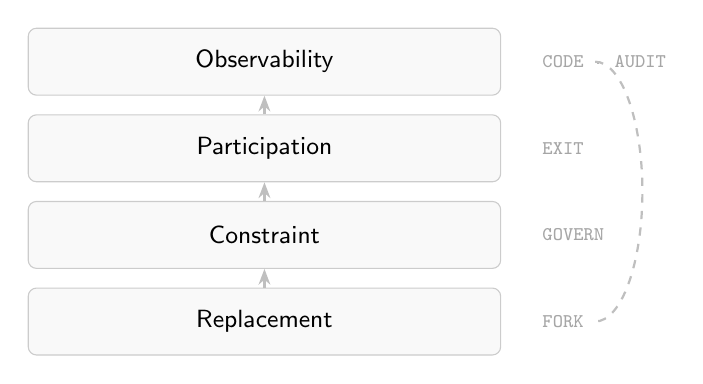
\begin{tikzpicture}[
    layer/.style={rectangle, draw=gray!40, fill=gray!5, rounded corners=3pt, minimum width=6cm, minimum height=0.85cm, font=\sffamily\small},
    testlabel/.style={font=\ttfamily\scriptsize, text=gray!70},
    arrow/.style={-{Stealth[length=2mm]}, thick, gray!50}
]

% Four layers (top to bottom, matching SVG order)
\node[layer] (obs) at (0, 3.3) {Observability};
\node[layer] (part) at (0, 2.2) {Participation};
\node[layer] (cons) at (0, 1.1) {Constraint};
\node[layer] (repl) at (0, 0) {Replacement};

% Test labels (right side, monospace)
\node[testlabel, right=0.4cm of obs.east, anchor=west] {CODE \textperiodcentered{} AUDIT};
\node[testlabel, right=0.4cm of part.east, anchor=west] {EXIT};
\node[testlabel, right=0.4cm of cons.east, anchor=west] {GOVERN};
\node[testlabel, right=0.4cm of repl.east, anchor=west] {FORK};

% Upward arrows between layers
\draw[arrow] (repl.north) -- (cons.south);
\draw[arrow] (cons.north) -- (part.south);
\draw[arrow] (part.north) -- (obs.south);

% Curved feedback loop (right side, dashed)
\draw[gray!50, thick, dashed]
    (4.2, 3.3) arc[start angle=90, end angle=-90, x radius=0.6cm, y radius=1.65cm];

\end{tikzpicture}
\caption{\textbf{Closed-Loop Corrigibility Architecture.} Four control layers form a closed feedback loop. Removal of any layer converts the system to open-loop, permitting unbounded error accumulation.}
\label{fig:four-layers}
\end{figure}

\begin{figure}[htbp]
\centering
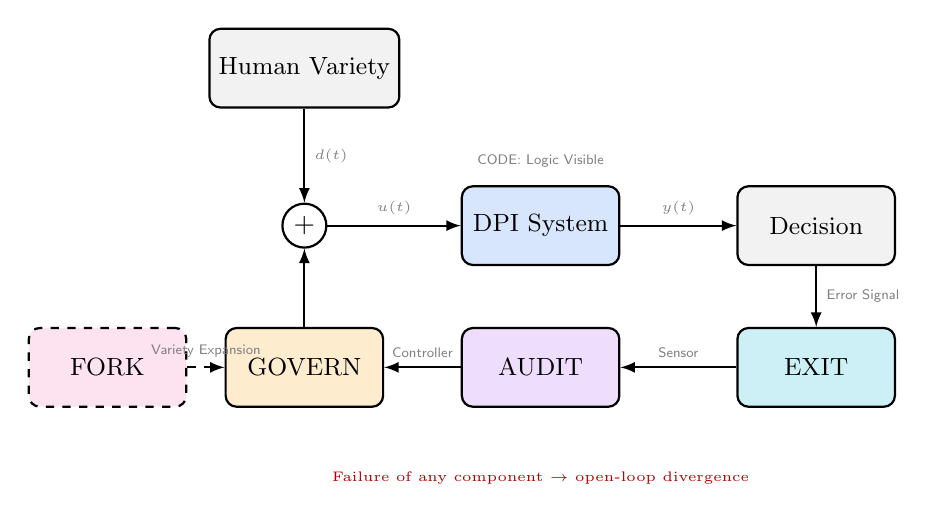
\begin{tikzpicture}[
    node distance=1.6cm, auto, >=latex, thick,
    block/.style={draw, rectangle, minimum height=1cm, minimum width=2cm, rounded corners, font=\small},
    sum/.style={draw, circle, inner sep=2pt},
    label/.style={font=\tiny\sffamily, text=gray}
]
    % Main flow
    \node[block, fill=gray!10] (disturbance) at (0, 2) {Human Variety};
    \node[sum] (sum1) at (0, 0) {$+$};
    \node[block, fill=codecolor!20] (plant) at (3, 0) {DPI System};
    \node[block, fill=gray!10] (output) at (6.5, 0) {Decision};

    % Feedback path
    \node[block, fill=exitcolor!20] (exit) at (6.5, -1.8) {EXIT};
    \node[block, fill=auditcolor!20] (audit) at (3, -1.8) {AUDIT};
    \node[block, fill=governcolor!20] (govern) at (0, -1.8) {GOVERN};

    % FORK as expansion
    \node[block, fill=forkcolor!20, dashed] (fork) at (-2.5, -1.8) {FORK};

    % CODE overlay
    \node[label, above=0.1cm of plant] {CODE: Logic Visible};

    % Connections - forward path
    \draw[->] (disturbance) -- node[right, label] {$d(t)$} (sum1);
    \draw[->] (sum1) -- node[above, label] {$u(t)$} (plant);
    \draw[->] (plant) -- node[above, label] {$y(t)$} (output);

    % Connections - feedback path
    \draw[->] (output) -- node[right, label] {Error Signal} (exit);
    \draw[->] (exit) -- node[above, label] {Sensor} (audit);
    \draw[->] (audit) -- node[above, label] {Controller} (govern);
    \draw[->] (govern) -- (sum1);

    % FORK expansion
    \draw[->, dashed] (fork) -- node[above, label] {Variety Expansion} (govern);

    % Annotations
    \node[font=\tiny, text=red!70!black, align=center] at (3, -3.2) {Failure of any component $\rightarrow$ open-loop divergence};
\end{tikzpicture}
\caption{\textbf{Corrigibility as a Closed-Loop Control Architecture.} Digital Public Infrastructure is modeled as a feedback control system subject to continuous human and environmental disturbance. Corrigibility requires that error signals (EXIT) remain detectable, that system behavior be intelligible (CODE), that sensing mechanisms be transparent (AUDIT), that binding corrective authority exist (GOVERN), and that structural reproduction be feasible (FORK). Failure of any single component collapses the loop into open-loop operation. Under non-zero integrating disturbance, error diverges unboundedly (Null-Feedback Instability, Proposition~\ref{thm:null-feedback}; Appendix~\ref{appendix:proofs}). Corrigibility is therefore a structural property of loop integrity, not a matter of operator intent.}
\label{fig:control-loop}
\end{figure}

\subsection{Test 1: EXIT (Reversibility of Participation)}

\begin{definition}[EXIT]
\label{def:exit}
A system $S$ satisfies \textbf{Reversibility of Participation} if, for any user in state $s \in S$, there exists a transition to a non-participatory state $s_0$ such that the penalty $\pi(s \to s_0)$ is strictly bounded: $\pi(s \to s_0) < \tau_{\text{exit}}$, where $\tau_{\text{exit}}$ is a threshold below which the penalty does not constitute material exclusion from essential services. For essential systems, where no bounded-penalty $s_0$ can exist (Proposition~\ref{prop:essentiality}), the test is dischargeable in exactly one other way: verified Functional Exit Equivalence (Section~\ref{subsubsec:fee}), which recreates the error-signal strength literal exit would have supplied. The test remains binary --- bounded-penalty exit, or verified FEE, or failure.
\end{definition}

The foundational condition of any corrigible system is the \textbf{Reversibility of Participation}. Irrevocable consent functions structurally as mandatory lock-in. For an infrastructure to operate as a public utility rather than a coercive instrument, users must possess the capacity to withdraw from it without incurring disproportionate penalty or material exclusion.

In practice, many systems operate as a ratchet. They are easy to enter but functional imperatives make them impossible to leave. \textbf{Aadhaar} exemplifies this failure: opting out results in exclusion from subsidized food rations under the upheld Section 7 linkage, and --- although \textit{Puttaswamy~II} (2018) struck down mandatory linking for bank accounts and SIM cards --- de facto insistence on Aadhaar at the point of service persists across banking and connectivity \citep{khera2019}. When a system becomes a prerequisite for existence, refusal results in a disproportionate survival penalty rather than functioning as feedback. \textbf{UPI} partially mitigates this because cash remains legal tender, but network effects increasingly marginalize non-participants. \textbf{Linux}, by contrast, imposes no survival penalty: a user can migrate to BSD or Windows without losing access to essential services.

From a cybernetic perspective, EXIT constitutes the primary negative feedback loop. Blocking this channel silences the user's error signal. This blockade overloads the political layer with demands that the technical layer has suppressed.

This dynamic was formalized by Hirschman \citep{hirschman1970} in his analysis of organizational decline. Hirschman distinguished two correction mechanisms: exit (withdrawal from participation) and voice (attempts to change the system from within). His central finding is that these mechanisms exist in productive tension, not as substitutes.

Exit, in Hirschman's formulation, is ``neat,'' ``impersonal,'' and ``indirect'': one either exits or one does not. This binary quality makes exit a high-bandwidth error signal. When users leave, the system receives unambiguous information that something has failed. Voice, by contrast, is costly and conditioned on the influence and bargaining power that participants can bring to bear. Voice is gradual, political, and requires sustained effort.

Critically, Hirschman demonstrated that exit without voice produces abandonment rather than correction: quality-conscious users flee rather than fight. But voice without exit produces capture: complaints become cosmetic (see Section~\ref{subsec:grievance}) because the system faces no credible threat of user departure. The effectiveness of voice depends on the credibility of exit.

This framework illuminates why mandatory enrollment is structurally pathological. By eliminating exit, a system does not merely suppress one feedback channel. It degrades voice itself. When citizens cannot leave, their complaints lack credibility. The operator can absorb infinite grievance without modifying system behavior ($\partial S / \partial G = 0$). Hirschman's insight formalizes what cybernetics predicts: blocking the error signal does not eliminate the error; it eliminates the system's capacity to respond.

\subsection{Test 2: CODE (Inspectability of Logic)}

\begin{definition}[CODE]
\label{def:code}
A system $S$ satisfies \textbf{Inspectability of Logic} if, for any decision function $f: X \to Y$ that determines user outcomes, there exists a publicly accessible artifact $A_f$ such that $A_f$ fully specifies the computation of $f(x)$ for all inputs $x \in X$.
\end{definition}

Users who cannot leave a system must possess the ability to inspect it. \textbf{Inspectability of Logic} requires that the rules determining outcomes are visible to those they govern. Power in a digital system resides in execution. Lessig \citep{lessig2006} established that software architecture functions as regulation: code ``determines what people can or cannot do in the first place,'' unlike legal regulation which sets rules for behavior and retroactively punishes non-compliance. This is regulation without appeal. If the execution path remains hidden, that power is absolute; it is not merely unaccountable but structurally unobservable to those it governs.

Transparency specifications or open standards are insufficient if the executing artifact remains a black box. \textbf{Aadhaar's} CIDR (Central Identities Data Repository) is proprietary: the matching algorithm that determines identity cannot be examined. \textbf{UPI} publishes API specifications, but the NPCI switching logic remains closed. \textbf{Let's Encrypt} demonstrates the alternative: its CA software is fully open source, allowing anyone to audit the certificate issuance logic that secures web traffic.

\subsection{Test 3: AUDIT (Independent Verification)}

\begin{definition}[AUDIT]
\label{def:audit}
A system $S$ satisfies \textbf{Independent Verification} if any external party $P$, without requiring operator authorization, can measure the system's error rate $\epsilon_S$, verify compliance with stated specifications, and document failure modes in production environments. Formally: $\forall P: \text{Access}(P, \epsilon_S) = \text{true}$ without $\text{Authorize}(\text{Operator}, P)$.
\end{definition}

While inspection enables understanding, \textbf{Independent Verification} enables truth. This functions as the sensor in the cybernetic feedback loop. A system is verifiable only if external, permissionless actors can test its behavior, measure its error rates, and document its failure modes within production environments.

\begin{remark}[The Auditability Distinction]
The framework does not equate auditability with direct participation. AUDIT $\neq$ ``everyone audits''; AUDIT $=$ ``no one can prevent auditing.'' \textbf{Journalism analogy:} Not everyone investigates corruption. Democracy still depends on the \textit{possibility} of investigation. The problem today is not that auditors exist; operators can legally block them. The tradeoff is contestable expertise over unchallengeable authority, a defensible democratic position.
\end{remark}

Ostrom's design principles require that monitors be accountable to appropriators, not external authorities \citep{ostrom1990}. Applied to DPI: audit capacity must be exercisable by affected communities or their designated agents, not delegated exclusively to operator-approved auditors or captured regulatory bodies.

\paragraph{Intermediary-Discretion Surface.} The AUDIT surface extends to every rung of the implementation chain, not only to the system operator. In practice, the layer between the operator and the affected person --- ration dealers, enrollment-camp operators, local-office clerks, vendor integration partners --- exercises delegated discretion that determines whether the system's stated behavior reaches the citizen. Aggregate error-rate metrics ($\epsilon_S$ system-wide) can certify AUDIT as passing for the operator while a particular implementation rung sustains a locally captured regime invisible to system-level measurement. The audit surface must therefore include: (i) per-node or per-agent variance in denial, exception, and manual-override rates, with statistical outlier detection as a mandatory audit output; (ii) a disclosure requirement that the operator enumerate every role holding delegated discretion over subject outcomes, with each role's documented revocation and appeal path; and (iii) Rule~A.9 enforcement-history evidence applied to sanctions against intermediaries, not only against the operator. An audit that measures only the system's aggregate behavior has not measured the layer through which the governed actually encounter it.

Incorrigible systems typically capture this function. \textbf{UPI} permits RBI regulatory audits, but transaction-level verification requires NPCI authorization; independent researchers cannot measure failure rates or dispute resolution times. \textbf{Proprietary cloud services} (AWS, Azure, GCP) publish compliance certifications while blocking independent verification of infrastructure behavior at scale. \textbf{Bitcoin} provides the counter-model: every transaction is independently verifiable by any node, and consensus is cryptographic proof. Similarly, \textbf{Let's Encrypt} publishes Certificate Transparency logs, making every issued certificate publicly auditable in real time.

The structural function of opacity is sensor failure. A system whose error rates cannot be independently measured cannot be regulated. The controller receives no signal about divergence from intended behavior. Under Ashby's Law, such a system will drift until external forces impose correction. Those forces, operating outside the technical loop, will impose correction through channels the system cannot anticipate or absorb. \citet{pasquale2015} describes this as a ``one-way mirror'' relationship, but the cybernetic translation is precise: asymmetric observability breaks the feedback loop at the sensing stage.

\subsection{Test 4: GOVERN (Constitutive Constraint)}

\begin{definition}[GOVERN]
\label{def:govern}
A system $S$ satisfies \textbf{Constitutive Constraint} if there exists a governance function $G: \text{Rules} \to \text{Rules}'$ such that (1) $G$ is accessible to affected parties, not solely the operator; (2) $G$ is binding, meaning the operator cannot override $G$'s output; and (3) there exists a cryptographic or legal chain of custody linking system behavior to $G$'s constraints.
\end{definition}

Verification identifies the error, while \textbf{Constitutive Constraint} enforces the correction. This framework distinguishes structural governance from administrative functions like consultation, multi-stakeholder meetings, or feedback forms.

Governance exists only when binding constraints limit system behavior in ways the operator cannot override. \textbf{Aadhaar} is governed by UIDAI fiat: the same entity that operates the system sets its rules. \textbf{UPI} has NPCI governance, but NPCI is majority-owned by participating banks, creating structural conflicts. \textbf{Let's Encrypt} shows what binding constraint looks like: the ISRG charter legally binds the organization to its public benefit mission, with community board representation. \textbf{Bitcoin's} BIP process demonstrates governance through proven fork history; contentious changes have been rejected by the network, proving the community can override developer intent. \textbf{PostgreSQL's} permissive license and distributed core-team governance --- no single corporate copyright holder, no contributor license agreement --- prevent any single entity from capturing the project.

\subsubsection{The Post-Execution Fallacy}
\label{subsec:post-execution}
A critical failure in modern policy involves relying on exogenous or post-hoc remedies to substitute for structural constraints. Mechanisms such as courts, ombudsmen, and grievance redressal officers operate on ``bureaucratic time,'' measured in months or years. Infrastructure operates on ``digital time,'' measured in milliseconds. A system that executes a harmful action, such as wrongful deletion of a beneficiary, and relies on a court order to reverse it six months later is structurally ungoverned for that duration. True governance must function within the system's execution loop to block prohibited states before they manifest.

Consequently, claims of governance must be evidentiary rather than declarative. They require a signed cryptographic chain of custody linking the operator's authority to an external, non-overrideable instrument.

\subsubsection{Strategic Openness vs Structural Accountability}

Open artifacts do not guarantee open governance. Systems can deploy \textit{asymmetric openness}: releasing code or weights for ecosystem adoption while retaining governance control. This pattern (detailed in Section~\ref{sec:diagnosis}) satisfies CODE while failing GOVERN. The GOVERN test requires bidirectional accountability: not merely that citizens can observe the system, but that they can correct it. A system that publishes its code while reserving all governance decisions to the operator has satisfied CODE but failed GOVERN.

A related confusion conflates governing one's own data with governing the system itself. Data protection frameworks (GDPR, CCPA) grant users rights to access, correct, delete, and port their data. These rights are necessary but insufficient: they allow users to manage information within rules the operator defines, not to change those rules. The GOVERN test asks: can affected parties change the rules, not merely operate within them?

\subsection{Test 5: FORK (Independent Reproduction)}

\begin{definition}[FORK]
\label{def:fork}
A system $S$ satisfies \textbf{Independent Reproduction} if an independent party can instantiate a functionally equivalent system $S'$ such that (1) no legal prohibition prevents $S'$'s deployment; (2) the artifacts required for reproduction (code, schemas, protocols) are publicly available; and (3) user state $U_S$ is portable: $U_S \to U_{S'}$. For deterministic infrastructure, natural barriers (capital, network effects) do not disqualify FORK; only constructed barriers (legal prohibition, regulatory monopoly, deliberate technical enclosure) do. For learned systems, the companion paper shows that reproduction cost itself enters the test: resource asymmetry beyond a policy threshold (Compute and Data Capture) fails FORK regardless of licensing terms~\citep{aravind2026epi}.
\end{definition}

The ultimate check on power is the ability to recreate it. \textbf{Independent Reproduction} determines whether the ecosystem allows the infrastructure itself to be separated from its current steward. This requirement distinguishes structural resilience from simple market competition.

\begin{remark}[Credible Replaceability]
The paper does not define FORK as ``routine divergence in production.'' It defines FORK as \textbf{credible replaceability in extremis}. \textbf{Constitutional analogy:} The US Constitution is forkable (amendable, secession historically possible). That does not mean every county runs a different constitution. The \textit{possibility} disciplines the center. \textbf{The stable equilibrium:} Latent forkability + strong coordination incentives. Email works not because everyone forks SMTP, but because anyone \textit{could}. \textbf{Key asymmetry:} FORK is a threat, not a preference. No one wants fragmentation. But irreversibility without exit is worse.
\end{remark}

The existence of competitors, such as choosing between two proprietary cloud providers, provides an ``Exit'' option but not a ``Fork.'' Shifting providers allows a user to escape a specific operator, but it forces them to abandon their history, identity, and operational logic. This action is substitution, not reproduction.

\subsubsection{Natural vs Constructed Barriers}

A critical distinction must be drawn between barriers to forking that are \textbf{natural} (arising from coordination costs, network effects, or capital requirements) and those that are \textbf{constructed} (arising from legal prohibition, regulatory monopoly, or deliberate technical enclosure).

\begin{itemize}
    \item \textbf{Natural barriers}: Gmail dominates email not because forking SMTP is illegal, but because Google invested in spam filtering and UX. Anyone \textit{can} run their own mail server. Network effects and capital create friction, but not prohibition.
    \item \textbf{Constructed barriers}: NPCI is the \textit{only permitted} instant payment switch in India. The barrier is regulatory, not economic. Even with infinite capital, you cannot legally compete with UPI's core switching function.
    \item \textbf{Grant-conditioned barriers}: Sri Lanka's MOSIP implementation is contractually restricted to donor-country system integrators, despite MOSIP's open-source license \citep{biometricupdate2025}. The barrier is neither regulatory nor technical but financial: grant conditions foreclose supplier choice, demonstrating how ``open'' DPI exports can create new dependencies.
\end{itemize}

The FORK test fails only when constructed barriers prevent reproduction. Natural barriers reduce the \textit{likelihood} of forking; constructed barriers eliminate its \textit{possibility}. A system with high natural barriers but no constructed barriers (Linux, email) remains structurally corrigible. A system with low natural barriers but constructed prohibition (hypothetically: open-source software banned by law) would fail FORK despite technical simplicity.

\subsubsection{State Portability as a Precondition for Fork}

A critical structural requirement: code forkability is insufficient if \textbf{user state} is non-transferable. In traditional software (Linux, PostgreSQL), the artifact being forked \textit{is} the system. In Digital Public Infrastructure, the artifact is merely the skeleton; the system includes the user's credentials, transaction history, social graph, and accumulated trust relationships.

Let $U_S$ denote the user state graph in system $S$, and $S'$ a forked alternative. A fork is \textbf{functionally meaningful} only if:

\begin{equation}
U_S \to U_{S'} \quad \text{(state portability)}
\label{eq:state-portability}
\end{equation}

Open code with locked data produces a hollow fork. The legal right to reproduce an identity system is meaningless if citizens cannot port their credentials, attestations, and service eligibility to the new instance.

\paragraph{Switching Cost and Portability.} The practical barrier to exit and fork can be assessed through \textbf{switching cost}: the aggregate friction of data export, service downtime, credential re-establishment, network loss, and legal barriers. When switching cost to all plausible alternatives exceeds a policy threshold, EXIT and FORK functionally fail regardless of formal rights. Aadhaar exhibits near-maximal switching cost: no data export exists, service denial during transition is total, and legal mandate forecloses alternatives. UPI retains lower switching cost because cash and cards remain legal. The formal operationalization appears in Appendix~\ref{appendix:proofs}.

\paragraph{Technical Requirements for Portability.} To ensure meaningful forkability, DPI systems must implement: (1) standardized export bundles with user-owned credentials, (2) interoperability APIs to accept ported data, and (3) statutory guarantees requiring public services to accept verified portable credentials. This is the lesson of PSD2 in banking: portability mandates made bank-switching economically viable.

A system passes the FORK test only if the community possesses the legal rights, technical artifacts, economic means, \textbf{and state portability guarantees} to spawn a functionally equivalent instance. License choice determines whether forkability persists across derivatives: copyleft licenses (GPL, AGPL) ensure modifications remain forkable; permissive licenses (MIT, Apache) allow derivatives to be enclosed. For network-deployed DPI, AGPL-style requirements prevent operators from capturing modified code behind service interfaces. \textbf{Aadhaar} fails completely: no entity outside UIDAI can reproduce the identity infrastructure. \textbf{OpenSearch} demonstrates what successful forking looks like. When Elastic changed its license, AWS forked Elasticsearch and the community continued development independently. \textbf{Linux} has been forked thousands of times (Android, Chrome OS, countless distributions). \textbf{AWS S3} presents partial forkability: the API specification is public and MinIO provides a compatible implementation, but the operational scale, global infrastructure, and integration ecosystem cannot be reproduced by most organizations. Table~\ref{tab:exit-fork-differentiation} illustrates the distinction across representative cases: substitution (EXIT) and reproduction (FORK) are independent properties, and a system can satisfy one while failing the other.

\begin{table}[htbp]
\centering
\begin{tabular}{@{}lllp{5.5cm}@{}}
\toprule
\textbf{System} & \textbf{EXIT} & \textbf{FORK} & \textbf{Structural Reality} \\
\midrule
Cloudflare & PASS & FAIL & Can switch to Fastly, cannot reproduce \\
AWS EC2 & PASS & FAIL & Can migrate to Azure, logic/state locked \\
Aadhaar & FAIL & FAIL & Cannot refuse, cannot reproduce \\
Linux & PASS & PASS & Can leave, can fork \\
AWS S3 & PASS & PARTIAL & API open (MinIO), scale unreproducible \\
\bottomrule
\end{tabular}
\caption{Differentiation between EXIT (substitution) and FORK (reproduction). EXIT requires only that an alternative service exists; FORK requires that the system itself can be independently reproduced. Many systems satisfy EXIT through substitution while failing FORK through irreproducibility, and the distinction matters under centralized-vendor lock-in.}
\label{tab:exit-fork-differentiation}
\end{table}

\subsection{Contestation of Representational Categories in AI-Mediated DPI}
\label{subsec:contestation}

The five tests presented above were derived for deterministic infrastructure: ledgers, registries, and rule-based engines. As DPI increasingly incorporates learned components, the GOVERN test acquires a second contestation surface that the deterministic case does not require. This subsection identifies that surface; the formal constraints on the learned-system side are developed in the companion paper~\citep{aravind2026epi}.

When learned systems are deployed within DPI, the categories they use to classify citizens (``eligibility,'' ``risk,'' ``fraud,'' ``vulnerability,'' ``priority'') cease to be mere statistical properties of a model. They become \textbf{consequential administrative determinations}. A citizen flagged as ``high-risk'' by an AI-mediated welfare system experiences that label as legal fact: payments suspended, services revoked, additional verification demanded. The label has the same operational force as a determination from a deterministic registry, even though it emerged from a probabilistic computation over an undisclosed feature space.

The structural problem is that affected communities must possess the capacity to \emph{review and contest the representational categories themselves}, not just dispute individual execution decisions. Representation in AI-mediated DPI differs fundamentally from representation in deterministic administrative systems: the categories are \textbf{emergent rather than deliberately designed}. In a deterministic registry, ``eligibility'' is defined by a rule the legislature wrote; the contestation surface is the rule's text. In a learned system, ``eligibility'' is defined by the joint distribution of training data, loss function, and inference pipeline; the contestation surface is the schema, the data, and the model's operative representation simultaneously.

Three structural consequences follow:

\begin{enumerate}[noitemsep]
    \item \textbf{Per-decision appeal is necessary but insufficient.} A citizen who successfully appeals one classification has not contested the category that produced it. The next million decisions will be drawn from the same category. Adequate contestation requires standing to challenge the schema, not just the application of the rule.
    \item \textbf{Disclosure obligations extend to the operative representation.} Publishing model weights does not satisfy GOVERN if the categorical structure that emerges at inference time is undisclosed. The state retains nominal authority over the rule but loses substantive authority over the categories that animate it.
    \item \textbf{Standing must include the affected class, not only the operator.} Because the schema captures the population's classification surface, contestation rights cannot be confined to procurement disputes between the state and the vendor. Affected populations must hold standing to challenge the representational schema directly.
\end{enumerate}

\begin{remark}[Extension of GOVERN to Ontological Choices]
\label{rem:govern-ontological}
The GOVERN test extends to ontological choices when those choices produce binding classifications. An AI-mediated DPI deployment satisfies GOVERN only if affected populations can challenge the categorical schema, not merely dispute individual outputs. The formal constraints required to render this contestation operative (LWD-R disclosure, operative-representation transparency, action-boundary auditability) are developed in the companion paper's analysis of learned-system corrigibility~\citep{aravind2026epi}.
\end{remark}

\paragraph{Collective-Standing Precondition (Ostrom Principle~7).} Ostrom's seventh design principle, the minimal recognition of the right to organize, is a precondition for the mechanism families through which GOVERN operates at population scale: class-action vehicles, deliberative forums, and juridical standing all presuppose that affected parties can constitute themselves as a collective actor, with rights to associate, aggregate claims, and fund representation. The framework's GOVERN test verifies the channel; Principle~7 verifies whether the subject that uses the channel can be constituted. Where the right to organize is suppressed --- by association law, administrative harassment, cost barriers that foreclose legal aggregation, or structural atomization --- the formal availability of GOVERN mechanisms does not translate into operative corrective authority, and the loop is open in fact even when the channel is structurally present. GOVERN determinations therefore carry the implicit precondition that this associational capacity is legally protected and historically exercised at the relevant stratum (Rule~A.9 evidence standard). Where this precondition fails, the audit must record GOVERN as failing at that stratum and document the associational constraint as the cause. Individual grievance pathways are not substitutes; they address individual cases without generating the collective error signal that governance correction requires.

This bridge clause completes the deterministic framework's account of the GOVERN test for the AI era: the test does not change, but its evidentiary burden does. The companion paper takes up the verification machinery in detail and develops a strict-interpretability firewall: when the operative representation of a learned component cannot be disclosed to the standard required for auditable reproduction, the system fails CODE for high-stakes deployments and should not, consistent with this framework's legitimacy criteria, be adopted as Epistemic Public Infrastructure in rights-affecting tiers \citep{aravind2026epi}.

\subsection{The Topology of Necessity}

Five tests describe the anatomy of a stable control loop rather than a random assortment of normative virtues (see Figure~\ref{fig:control-loop}).

\begin{itemize}[noitemsep,topsep=0pt]
    \item \textbf{EXIT} provides the Error Signal.
    \item \textbf{AUDIT} acts as the Sensor.
    \item \textbf{CODE} ensures Transmission Clarity.
    \item \textbf{GOVERN} serves as the Actuator.
    \item \textbf{FORK} provides Selection Pressure over the entire loop.
\end{itemize}

Failure in any single dimension breaks the control loop at a specific physical point. The result is not partial infrastructure but \textbf{Open Loop Control}. An open-loop system executes directives without the capacity to sense deviation, interpret error, or apply corrective force.

\paragraph{Failure-Dominated Structure.} Corrigibility is failure-dominated. If any single constraint collapses, corrective authority becomes contingent rather than guaranteed. This weakest-link structure mirrors distributed systems reliability: system safety is bounded by the least reliable component. Under human variety and environmental change, open-loop control drifts toward failure.

Corrigibility closes the loop. Only when all five tests are satisfied does a system possess a complete feedback topology capable of detecting divergence, transmitting intelligible signals, executing correction, and replacing failed control logic when necessary. Without this closure, error correction is structurally discretionary, and bounded-error operation cannot be guaranteed.

\begin{figure}[H]
\centering
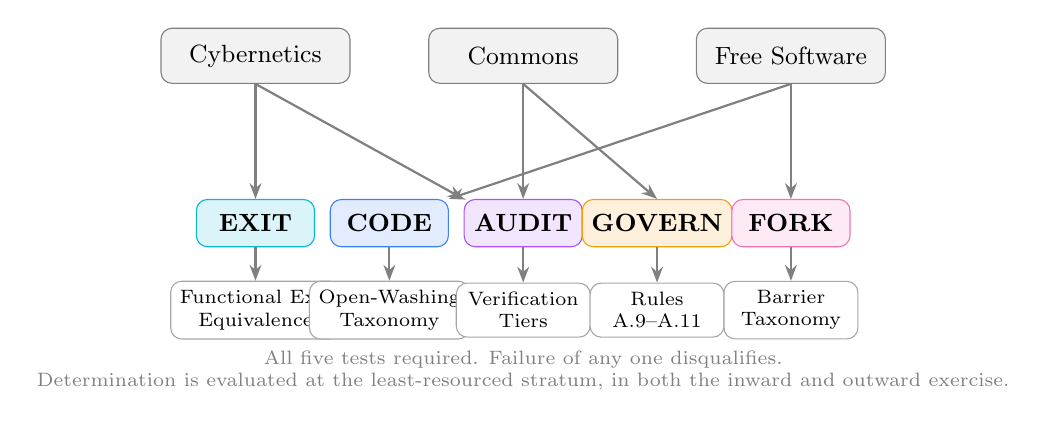
\begin{tikzpicture}[scale=0.85,
    tradition/.style={rectangle, rounded corners, draw=gray, fill=gray!10, minimum width=2.4cm, minimum height=0.7cm, font=\small},
    test/.style={rectangle, rounded corners, draw=#1, fill=#1!15, minimum width=1.5cm, minimum height=0.6cm, font=\small\bfseries},
    instrument/.style={rectangle, rounded corners, draw=gray!70, fill=white, minimum width=1.7cm, minimum height=0.55cm, font=\scriptsize, align=center},
    arrow/.style={-{Stealth[length=2mm]}, gray, thick}
]
% Three traditions at top
\node[tradition] (cyber) at (0,2.5) {Cybernetics};
\node[tradition] (commons) at (4,2.5) {Commons};
\node[tradition] (foss) at (8,2.5) {Free Software};

% Five tests in the middle
\node[test=exitcolor] (exit) at (0,0) {EXIT};
\node[test=codecolor] (code) at (2,0) {CODE};
\node[test=auditcolor] (audit) at (4,0) {AUDIT};
\node[test=governcolor] (govern) at (6,0) {GOVERN};
\node[test=forkcolor] (fork) at (8,0) {FORK};

% Connections - Cybernetics
\draw[arrow] (cyber.south) -- (exit.north);
\draw[arrow] (cyber.south) -- (audit.north west);

% Connections - Commons
\draw[arrow] (commons.south) -- (audit.north);
\draw[arrow] (commons.south) -- (govern.north);

% Connections - FOSS
\draw[arrow] (foss.south) -- (code.north east);
\draw[arrow] (foss.south) -- (fork.north);

% Verification instruments derived from the tests
\node[instrument] (i-exit) at (0,-1.3) {Functional Exit\\Equivalence};
\node[instrument] (i-code) at (2,-1.3) {Open-Washing\\Taxonomy};
\node[instrument] (i-audit) at (4,-1.3) {Verification\\Tiers};
\node[instrument] (i-govern) at (6,-1.3) {Rules\\A.9--A.11};
\node[instrument] (i-fork) at (8,-1.3) {Barrier\\Taxonomy};

\draw[arrow] (exit.south) -- (i-exit.north);
\draw[arrow] (code.south) -- (i-code.north);
\draw[arrow] (audit.south) -- (i-audit.north);
\draw[arrow] (govern.south) -- (i-govern.north);
\draw[arrow] (fork.south) -- (i-fork.north);

% Labels
\node[font=\scriptsize, gray, align=center] at (4,-2.2) {All five tests required. Failure of any one disqualifies.\\Determination is evaluated at the least-resourced stratum, in both the inward and outward exercise.};
\end{tikzpicture}
\caption{The framework at a glance. Three independent theoretical traditions (top) derive the five corrigibility tests (middle), and the tests in turn derive their verification instruments (bottom): Functional Exit Equivalence (Section~\ref{subsubsec:fee}), the open-washing taxonomy, verification tiers, the evidence rules of Appendix~\ref{appendix:rules}, and the constructed-versus-natural barrier taxonomy. Determination is evaluated at the least-resourced stratum (Remark~\ref{rem:argmin}) and in both the inward and outward exercise of each test.}
\label{fig:framework}
\end{figure}

\subsection{Structural Symmetry of Power}

The five tests, while derived from distinct intellectual traditions (Figure~\ref{fig:framework}), share a common organizing principle. Each enforces a constraint on power concentration at a different layer of the system. Together, they form a single power invariant:

\begin{center}
\begin{tabular}{@{}lll@{}}
\toprule
\textbf{Layer} & \textbf{Test} & \textbf{Function (Cybernetic)} \\
\midrule
Participation & EXIT & Reversibility of participation \\
Observability & CODE & Inspectability of rules \\
Observability & AUDIT & Verifiability of error \\
Constraint & GOVERN & Constraint on controller variance \\
Replacement & FORK & Selection pressure via reproduction \\
\bottomrule
\end{tabular}
\end{center}

Each test enforces the same principle: \textit{No actor exercising power may be the sole judge of its continuation, scope, or correction.}

A system without EXIT is coercive. A system without GOVERN is arbitrary. A system without FORK is captive.

\subsection{The Dual Exercise of the Tests}
\label{subsec:dual-exercise}

Each test admits two exercises, distinguished by who holds the corrective capacity. The \textbf{inward exercise} belongs to parties at or inside the operator's institutional perimeter --- the operator's own controls, its auditors, its regulator. The \textbf{outward exercise} belongs to the subject the system decides about: the participant whose error signal the loop exists to carry. The five definitions in this section are stated in the outward voice --- refusal, inspection, verification, constraint, and reproduction are capacities of affected participants. The verification apparatus that discharges them (manifests, audit rules, evidence standards; Appendices~\ref{appendix:architecture} and~\ref{appendix:rules}) operates largely in the inward voice. The gap between the two voices is where corrigibility claims most often fail in practice: a deployment can satisfy every test through inward instruments and remain unreachable from the outside.

\begin{table}[htbp]
\centering
\small
\caption{The dual exercise of each test. Inward instruments enforce; outward instruments carry the error signal the enforcement exists to serve. Under the weakest-link principle, a test discharged only inward has been verified for the operator, not for the governed --- the gradient quantifier (Remark~\ref{rem:argmin}) restated at the instrument level.}
\label{tab:dual-exercise}
\begin{tabular}{@{}lp{5.2cm}p{5.2cm}@{}}
\toprule
\textbf{Test} & \textbf{Inward exercise (operator, auditor, regulator)} & \textbf{Outward exercise (the governed)} \\
\midrule
EXIT & Halt, suspension, deprovisioning of the system's own components & Refusal without disproportionate penalty (Definition~\ref{def:exit}); Functional Exit Equivalence for essential services (Section~\ref{subsubsec:fee}) \\
CODE & Source access for audit teams; reproducible builds & Rules legible to the person they decide: the operative rule in a subject's case is identifiable and stated \\
AUDIT & Permissionless verification by external parties (Rule~A.10 chain of custody) & Notice that a decision occurred, and a record the subject can verify against the lived event~\citep{aravind2026epi}, under purpose-bound data duties (Rule~A.11) \\
GOVERN & Binding charter with enforcement history (Rule~A.9) & Contestation with binding effect, including the categorical schema (Section~\ref{subsec:contestation}); collective standing as precondition \\
FORK & Legal rights, artifacts, and resources for independent reproduction & State portability of the subject's own credentials and history (Equation~\ref{eq:state-portability}); acceptance of the ported record \\
\bottomrule
\end{tabular}
\end{table}

The columns are not alternatives, and the inward column is not a deficiency. Enforcement machinery, independent audit, and regulatory teeth are how correction is executed, and nothing reaches the subject without them. The failure mode is substitution, treating the inward column as the whole of the test. Consider a system whose operator can halt it, whose auditors can verify it, and whose regulator can bind it, while its subjects cannot refuse it, learn the rule that decided their case, confirm the record, contest the category, or carry their state elsewhere. That system is governed by its operator and incorrigible to the people it operates on. The inward column is how the operator governs the system. The outward column is how the governed correct the operator. Corrigibility is the second, standing on the first.

\subsection{Layer-Decomposed Evaluation}
\label{subsec:layers}

Complex infrastructure frequently stratifies into distinct functional layers, each with independent governance, transparency, and reproducibility properties. In agentic deployments the stratification acquires a second axis, delegation depth, where one system's harness contains another's; the companion paper extends this decomposition to nested delegation~\citep{aravind2026epi}. The five tests must be applied to each layer separately when:

\begin{enumerate}[noitemsep,topsep=0pt]
    \item Different entities control different layers (protocol versus implementation versus trust framework)
    \item Transparency varies across layers (open protocol, closed switching logic)
    \item Forkability differs by layer (code is forkable, network effects are not)
\end{enumerate}

\subsubsection{Propagation Rule}

A system that passes a test at one layer but fails at another does not achieve ``partial'' compliance. It fails the test. The evaluation proceeds from the layer closest to user impact upward; failure at any layer propagates to the whole.

Formally: Let $L_1, L_2, \ldots, L_n$ be the layers of a system, ordered by proximity to user impact. For test $T$:

\begin{equation}
T_{\text{system}} = \bigwedge_{i=1}^{n} T(L_i)
\label{eq:layer-propagation}
\end{equation}

The system passes $T$ if and only if every layer passes $T$. The full corrigibility determination extends this across all five tests:

\begin{equation}
\text{Corrigible}(S) = \bigwedge_{t \in \mathcal{T}} \bigwedge_{i=1}^{n} T_t(L_i) \quad \text{where } \mathcal{T} = \{\text{EXIT, CODE, AUDIT, GOVERN, FORK}\}
\label{eq:full-corrigibility}
\end{equation}

This double conjunction formalizes the ``weakest link'' principle: failure of any test at any layer propagates to the system determination.

\subsubsection{Application to Identity Infrastructure}

Table~\ref{tab:identity_layers} illustrates how layer decomposition applies to identity infrastructure: distinct architectural strata exhibit characteristically different failure modes that cannot be aggregated into a single system-wide judgment.

\begin{table}[htbp]
\centering
\small
\begin{tabular}{@{}llp{5cm}@{}}
\toprule
\textbf{Layer} & \textbf{Example Components} & \textbf{Typical Failure Mode} \\
\midrule
Protocol & W3C DID, VC Data Model & Often passes CODE \\
Implementation & Specific resolver, wallet software & May fail CODE (proprietary) \\
Credential & Issuer policies, attribute schemas & Often fails GOVERN (unilateral issuer) \\
Trust & Relying party acceptance, trusted lists & Often fails FORK (cannot reproduce acceptance) \\
\bottomrule
\end{tabular}
\caption{Identity infrastructure layer decomposition by vertical stratum. The DID-specific functional decomposition of the same stack is given in Table~\ref{tab:did_layers}.}
\label{tab:identity_layers}
\end{table}

The UPI payment rail exhibits similar layering: the protocol specification (NPCI-published) passes CODE at the protocol layer, but the switching logic (NPCI-operated) fails CODE at the implementation layer. Since the implementation layer is closer to user impact, the system fails CODE.

\subsubsection{The Weakest-Layer Principle}

This propagation rule has a counterintuitive but structurally necessary consequence: a system's corrigibility status equals its weakest layer across any test dimension. Strength at one layer cannot compensate for failure at another.

This principle prevents a common evasion: claiming corrigibility by publishing peripheral artifacts while retaining control over the layers that determine outcomes. Open-washing (Section~\ref{subsec:openwashing}) typically exploits layer confusion. Releasing SDKs (passing CODE at the interface layer) while keeping core logic proprietary (failing CODE at the execution layer) does not produce partial corrigibility. It produces total failure at the execution layer, which propagates to the system determination.

%% ============================================
%% SECTION 5: EMPIRICAL EVALUATION
%% ============================================

\section{Empirical Evaluation}
\label{sec:diagnosis}

The preceding sections established what corrigibility means and why it matters. Theory, however, must confront practice. Before analyzing \textit{why} systems fail these tests (the political economy, Section~\ref{sec:political-economy}), we first demonstrate \textit{that} they fail and document the human consequences. This section applies the five tests to real-world infrastructure, establishing the concrete stakes that motivate the analysis to follow. (The stress test of the same framework against learned systems is the companion paper~\citep{aravind2026epi}.)

To demonstrate the framework's application, we evaluate systems across three categories: government infrastructure promoted as ``DPI,'' platform infrastructure claiming ``openness,'' and infrastructure that satisfies all five tests.

\paragraph{A Note on Utility.} These evaluations assess structural accountability, not functional utility. A system can be simultaneously useful and incorrigible. Aadhaar may enable efficient service delivery; this does not establish that it permits correction by those it affects. The framework evaluates governance architecture, not operational performance. Utility and accountability are orthogonal dimensions: neither implies the other.

\subsection{Government Infrastructure: The Trap of Partial Compliance}

Government-operated systems currently designated as Digital Public Infrastructure frequently exhibit a dangerous failure mode: they achieve partial compliance on technical tests (EXIT, CODE, AUDIT) while failing structurally on governance tests (GOVERN, FORK). By capturing the monopoly on execution, they render the feedback loop inoperable.

\begin{table}[p]
    \centering
    \scriptsize
    \caption{\textbf{Evaluation of Government Infrastructure.} Centralized execution leads to consistent structural failure despite ``open standards'' rhetoric. PARTIAL is a diagnostic annotation only; in the binary determination it resolves to FAIL under the weakest-link principle (Equation~\ref{eq:full-corrigibility}, Section~\ref{subsec:methodology}).}
    \label{tab:govt_infra}

    % -- Subtable A: Aadhaar --
    \begin{subtable}{1\textwidth}
        \centering
        \caption{Aadhaar (India): Mandatory ID}
        \begin{tabular}{@{}llp{7cm}@{}}
            \toprule
            \textbf{Test} & \textbf{Result} & \textbf{Evidence} \\
            \midrule
            EXIT & $\times$ & Disproportionate penalty: statutory PDS linkage; de facto banking/SIM insistence post-\textit{Puttaswamy~II} \citep{khera2019}. \\
            CODE & $\times$ & Execution logic opaque: proprietary matcher, closed algorithms. \\
            AUDIT & $\times$ & External testing prohibited: independent error measurement illegal. \\
            GOVERN & $\times$ & No binding constraint: UIDAI is both operator and regulator. \\
            FORK & $\times$ & No legal/technical/economic means: total centralized capture. \\
            \bottomrule
        \end{tabular}
    \end{subtable}

    % -- Subtable B: UPI --
    \begin{subtable}{1\textwidth}
        \centering
        \caption{UPI (India): Payment Rail}
        \begin{tabular}{@{}llp{7cm}@{}}
            \toprule
            \textbf{Test} & \textbf{Result} & \textbf{Evidence} \\
            \midrule
            EXIT & \textcolor{orange}{PARTIAL} & Cash exists but network effects coerce. \\
            CODE & \textcolor{orange}{PARTIAL} & Protocol specs open, switching logic closed. \\
            AUDIT & \textcolor{orange}{PARTIAL} & Regulator audits, public measurement blocked. \\
            GOVERN & $\times$ & Banks own NPCI, regulate themselves. \\
            FORK & $\times$ & Hub-and-spoke requires NPCI cooperation. \\
            \bottomrule
        \end{tabular}
    \end{subtable}

    % -- Subtable C: Pix --
    \begin{subtable}{1\textwidth}
        \centering
        \caption{Pix (Brazil): Central Bank Payment}
        \begin{tabular}{@{}llp{7cm}@{}}
            \toprule
            \textbf{Test} & \textbf{Result} & \textbf{Evidence} \\
            \midrule
            EXIT & \textcolor{orange}{PARTIAL} & Cash/cards exist; digital-only services coerce. \\
            CODE & \textcolor{orange}{PARTIAL} & API spec public; central routing closed. \\
            AUDIT & \textcolor{orange}{PARTIAL} & Stats public; independent measurement blocked. \\
            GOVERN & $\times$ & BCB sets/enforces rules unilaterally. \\
            FORK & $\times$ & Central switch requires BCB. \\
            \bottomrule
        \end{tabular}
    \end{subtable}

    % -- Subtable D: X-Road --
    \begin{subtable}{1\textwidth}
        \centering
        \caption{X-Road (Estonia/Nordic): Data Exchange Layer}
        \begin{tabular}{@{}llp{7cm}@{}}
            \toprule
            \textbf{Test} & \textbf{Result} & \textbf{Evidence} \\
            \midrule
            EXIT & $\times$ & Exclusion from government services. \\
            CODE & $\checkmark$ & MIT source on GitHub. \\
            AUDIT & $\checkmark$ & Transaction logs, documented APIs. \\
            GOVERN & $\checkmark$ & NIIS treaty, MIT license irrevocable. \\
            FORK & $\checkmark$ & 25+ country deployments prove feasibility. \\
            \bottomrule
        \end{tabular}
    \end{subtable}

    % -- Subtable E: UK Open Banking --
    \begin{subtable}{1\textwidth}
        \centering
        \caption{UK Open Banking: Regulated API Standard}
        \begin{tabular}{@{}llp{7cm}@{}}
            \toprule
            \textbf{Test} & \textbf{Result} & \textbf{Evidence} \\
            \midrule
            EXIT & \textcolor{orange}{PARTIAL} & Can revoke API consent; cannot exit banking. \\
            CODE & $\times$ & Bank implementations proprietary. \\
            AUDIT & $\checkmark$ & FCA oversight, TPP certification. \\
            GOVERN & $\checkmark$ & CMA order, PSD2 regulation. \\
            FORK & \textcolor{orange}{PARTIAL} & Rights exist; means require regulatory approval. \\
            \bottomrule
        \end{tabular}
    \end{subtable}
\end{table}

\textbf{Pattern}: Pix (Brazil) illustrates how measurement frameworks mask structural failure. Global DPI assessments score Pix as the highest-aligned payment system in Latin America, meeting all eight payment-system variables spanning the six measured attributes \citep{ucl2025}. Yet Pix fails both GOVERN (Banco Central do Brasil sets and enforces rules unilaterally, with no binding citizen-corrective mechanism) and FORK (the central switch cannot be reproduced without BCB authorization). The variables measured---interoperability policy, participation conditions, oversight body---capture \textit{presence}, not \textit{function}. A citizen wrongly excluded from Pix has no structural path to correction beyond petitioning the same authority that excluded them. High measurement scores coexist with closed corrective loops.

Other government systems exhibit different failure patterns. X-Road (4/5) fails only EXIT: citizens cannot opt out of government data exchange, but the system passes CODE, AUDIT, GOVERN, and FORK \citep{xroad2026}. UK Open Banking (2/5) passes AUDIT and GOVERN but fails CODE: the API \textit{specification} is public, but the bank \textit{implementations} are proprietary. Specification $\neq$ Code. You can see the interface; you cannot inspect the execution.

\subsection{Platform Infrastructure: The Illusion of Openness}

In the private sector, systems often leverage ``open source'' branding while retaining centralized control. This decoupling of artifact transparency from governance reality creates a distinct failure pattern: the artifacts are public; the decisions are not. Table~\ref{tab:corp_infra} applies the five tests across cloud, social-platform, and identity-platform examples to make the pattern visible.

\begin{table}[htbp]
    \centering
    \scriptsize
    \caption{\textbf{Evaluation of Private/Platform Infrastructure.} Technical openness (Source Code/APIs) does not guarantee structural accountability. PARTIAL is a diagnostic annotation; in the binary determination it resolves to FAIL (Equation~\ref{eq:full-corrigibility}).}
    \label{tab:corp_infra}

    % -- Subtable A: Cloud Infrastructure (AWS/Azure) --
    \begin{subtable}{1\textwidth}
        \centering
        \caption{Cloud Infrastructure (AWS, Azure, GCP)}
        \begin{tabular}{@{}llp{7cm}@{}}
            \toprule
            \textbf{Test} & \textbf{Result} & \textbf{Evidence} \\
            \midrule
            EXIT & $\checkmark$ & Can migrate workloads to competing providers. \\
            CODE & \textcolor{orange}{PARTIAL} & APIs documented; internal routing/pricing opaque. \\
            AUDIT & \textcolor{orange}{PARTIAL} & Billing auditable; infrastructure logic unverifiable. \\
            GOVERN & $\times$ & Provider sets terms, regions, compliance unilaterally. \\
            FORK & $\times$ & Scale, global infrastructure unreproducible by states. \\
            \bottomrule
        \end{tabular}
    \end{subtable}

    % -- Subtable B: Android --
    \begin{subtable}{1\textwidth}
        \centering
        \caption{Android (AOSP + GMS)}
        \begin{tabular}{@{}llp{7cm}@{}}
            \toprule
            \textbf{Test} & \textbf{Result} & \textbf{Evidence} \\
            \midrule
            EXIT & \textcolor{orange}{PARTIAL} & Device portable; ecosystem lock-in creates friction. \\
            CODE & \textcolor{orange}{PARTIAL} & AOSP open; Play Services/Identity closed. \\
            AUDIT & \textcolor{orange}{PARTIAL} & OS auditable; Google Services opaque. \\
            GOVERN & $\times$ & Google sets roadmap/certification unilaterally. \\
            FORK & \textcolor{orange}{PARTIAL} & LineageOS exists; app ecosystem requires GMS. \\
            \bottomrule
        \end{tabular}
    \end{subtable}

    % -- Subtable C: Signal --
    \begin{subtable}{1\textwidth}
        \centering
        \caption{Signal Protocol}
        \begin{tabular}{@{}llp{7cm}@{}}
            \toprule
            \textbf{Test} & \textbf{Result} & \textbf{Evidence} \\
            \midrule
            EXIT & $\checkmark$ & Can switch to alternatives freely. \\
            CODE & $\checkmark$ & Client and server source available (GPL/AGPL). \\
            AUDIT & $\checkmark$ & Cryptographic properties independently verifiable. \\
            GOVERN & $\times$ & Foundation board sets direction unilaterally. \\
            FORK & $\times$ & State non-portable: no federation or graph export, so $U_S \to U_{S'}$ fails clause (3). \\
            \bottomrule
        \end{tabular}
    \end{subtable}
\end{table}

\textbf{Pattern: Asymmetric Openness.} These systems deploy strategic openness: releasing artifacts for ecosystem capture while retaining governance. This satisfies CODE (inspection possible) while failing GOVERN (correction blocked). The framework distinguishes artifact transparency (can you see the code?) from governance accountability (can you correct the system?). Open weights, open protocols, and open standards can each mask closed correction loops. ``Open weights'' $\neq$ ``open.'' ``Open source'' $\neq$ ``accountable.'' The artifact is open. The correction loop is closed. Seeing the machine does not govern it.

\subsection{Corrigible Infrastructure}

For contrast, Table~\ref{tab:positive} summarizes eighteen systems that pass all five tests. A striking pattern emerges: these systems are predominantly non-essential infrastructure. No individual's survival depends on accessing Linux or Let's Encrypt. This correlation between corrigibility and non-essentiality is not coincidental; it reflects a structural tension analyzed later in this paper.

\begin{table}[htbp]
\centering
\small
\renewcommand{\arraystretch}{1.3}
\begin{tabular}{@{}l>{\raggedright}p{3.2cm}>{\centering\arraybackslash}p{1.2cm}p{5.8cm}@{}}
\toprule
\rowcolor{gray!15}
\textbf{System} & \textbf{Steward} & \textbf{Score} & \textbf{Why Corrigible} \\
\midrule
\rowcolor{green!8}
Linux Kernel & Linux Foundation & \textbf{5/5} & Fully reproducible. Full triad (legal, technical, economic) exists. Independent distributions prove forkability. \\
Let's Encrypt & ISRG & \textbf{5/5} & Open source CA, IETF standards, nonprofit 501(c)(3) \\
\rowcolor{green!8}
Wikipedia & Wikimedia Foundation & \textbf{5/5} & CC BY-SA content, public edit history, community RfC governance \\
Matrix Protocol & Matrix.org Foundation & \textbf{5/5} & Apache 2.0, federated by design, self-hostable \\
\rowcolor{green!8}
Bluesky (AT Protocol) & Bluesky PBC & \textbf{5/5} & MIT/Apache; portable DID identity and self-hostable PDS make the fork threat credible, which is what binds PBC direction-setting (contrast Signal's GOVERN fail: no state portability, so no latent-fork discipline) \\
PostgreSQL & PGDG & \textbf{5/5} & BSD-like license, public mailing lists, major forks exist \\
\rowcolor{green!8}
IPFS & Protocol Labs & \textbf{5/5} & MIT/Apache, public IPIP process, no token governance \\
Bitcoin & Decentralized & \textbf{5/5} & MIT source, public BIP process, proven forks (BCH, BSV) \\
\rowcolor{green!8}
Kubernetes & CNCF & \textbf{5/5} & Apache 2.0, KEP process, distributions (OpenShift, k3s) \\
Firefox & Mozilla Foundation & \textbf{5/5} & MPL 2.0, nonprofit manifesto, forks (LibreWolf, Tor Browser) \\
\rowcolor{green!8}
Apache HTTP & Apache Foundation & \textbf{5/5} & Apache 2.0 license, ASF governance, powers 30\% of web \\
Apache Kafka & Apache Foundation & \textbf{5/5} & Apache 2.0, KIP process public, Fortune 500 standard \\
\rowcolor{green!8}
OpenSearch & Linux Foundation & \textbf{5/5} & Forked from Elasticsearch; Apache 2.0, multi-vendor governance \\
Valkey & Linux Foundation & \textbf{5/5} & Forked from Redis; BSD license, community governance restored \\
\rowcolor{green!8}
Hyperledger & LF Decentralized Trust & \textbf{5/5} & Apache 2.0 framework; institutional deployments require separate evaluation \\
LibreOffice & Document Foundation & \textbf{5/5} & Forked from OpenOffice; LGPL/MPL, nonprofit governance \\
\rowcolor{green!8}
MariaDB & MariaDB Foundation & \textbf{5/5} & Forked from MySQL; GPL, foundation governance \\
Eclipse IDE & Eclipse Foundation & \textbf{5/5} & EPL 2.0, 386 member orgs, committer-led governance \\
\bottomrule
\end{tabular}
\caption{Infrastructure systems satisfying all five corrigibility tests. The set is predominantly non-essential infrastructure, the pattern the essentiality analysis of Section~\ref{subsec:essential} explains.}
\label{tab:positive}
\end{table}

\textbf{Fork as Correction}: OpenSearch, Valkey, LibreOffice, and MariaDB demonstrate Ashby's Law in practice. Each emerged when governance variety collapsed: Oracle's Sun acquisition (2010) triggered LibreOffice and MariaDB; unilateral license changes triggered OpenSearch (2021) and Valkey (2024). The ecosystem restored requisite variety through forking.

The framework is governance-agnostic: corporate participation is not disqualifying. Kubernetes (CNCF), Hyperledger, and Let's Encrypt all have significant corporate involvement while passing all tests. The test is whether governance permits correction, not who participates.

\textbf{License vs. Governance}: Redis Ltd. added AGPLv3 in 2025, restoring open licensing. But license is orthogonal to governance. \textit{License} determines what you may do with code; \textit{governance} determines who decides what it becomes. Redis passes one; Valkey passes both.

\textbf{International Counterexample: Estonia's X-Road.} Estonia's X-Road architecture provides a counterexample demonstrating that scale does not necessitate centralized capture. Its federated data exchange model distributes control across institutional nodes, preserving CODE transparency (fully open-source, MIT license) and enabling institutional FORK at the implementation layer. While EXIT remains limited for certain core registries, the federated topology significantly reduces concentration coupling compared to monolithic architectures. X-Road has been adopted by Finland, Iceland, and deployed in more than twenty-five countries (Table~\ref{tab:govt_infra}), illustrating that corrigibility properties are architectural rather than cultural. The framework does not require cultural homogeneity or small population size; it requires federated governance that prevents single-point capture. (X-Road's full determination remains a fail on EXIT --- Section~\ref{subsubsec:arch-responses}; it appears here as the strongest near-miss among evaluated government systems, not as a pass.)

\subsection{The Taxonomy of Open-Washing}
\label{subsec:openwashing}

Systems that fail these structural tests frequently employ vocabulary to obscure their closure. The recurring patterns reduce to three strategic categories, each instantiated by several named tactics:

\begin{enumerate}
    \item \textbf{Symbolic-openness washing.} Substituting technical or diplomatic markers for governance accountability. Instances include \textit{Standard-Washing} (adopting open technical standards such as ISO/W3C as proxy for governance accountability), \textit{Open-Washing} (releasing peripheral SDKs while keeping core execution logic proprietary), \textit{Multilateral-Washing} (using G20/World Bank endorsements to substitute for technical auditability), and \textit{DID-Washing} (deploying decentralized identifiers without decentralized governance; see Section~\ref{subsubsec:didwashing}).
    \item \textbf{Coerced-legitimacy washing.} Grounding legitimacy in security narratives or coerced consent. Instances include \textit{Safety-Washing} (justifying opacity by claiming inspection poses a security risk) and \textit{Consent-Washing} (obtaining formal consent under conditions of economic coercion).
    \item \textbf{Substantive-substitution washing.} Invoking orthogonal public goods to legitimize structural changes that extend beyond the stated purpose. The principal instance is \textit{Climate-Washing} (using environmental rhetoric to legitimize movement, payment, or surveillance changes; see Section~\ref{subsubsec:climatewashing}).
\end{enumerate}

\subsubsection{DID-Washing: The Layer Confusion Problem}
\label{subsubsec:didwashing}

Decentralized Identifiers (DIDs) present a distinct challenge to corrigibility evaluation because they separate technical decentralization from governance decentralization across multiple architectural layers. The W3C DID Core 1.0 specification \citep{w3cdid2022} defines DIDs as ``globally unique identifiers'' that ``do not require a centralized registration authority.'' This technical claim is accurate. However, a system can implement DIDs at the identifier layer while retaining centralized control at every layer that determines actual utility.

Identity infrastructure comprises at least four functional layers, each with independent governance (Table~\ref{tab:did_layers}):

\begin{table}[htbp]
\centering
\small
\caption{DID infrastructure layers and typical corrigibility failures, by function. The vertical-strata decomposition of the identity stack is Table~\ref{tab:identity_layers}.}
\label{tab:did_layers}
\begin{tabular}{@{}lp{5cm}p{5cm}@{}}
\toprule
\textbf{Layer} & \textbf{Function} & \textbf{Common Failure} \\
\midrule
Identifier & DID generation, resolution & Often passes CODE (open specs) \\
Credential & Issuer policies, attribute schemas & Often fails GOVERN (unilateral issuer) \\
Wallet & Storage, presentation, consent & Often fails FORK (vendor lock-in) \\
Reliance & Verifier acceptance, trust frameworks & Often fails EXIT (no alternative verifiers) \\
\bottomrule
\end{tabular}
\end{table}

A system may achieve decentralization at the identifier layer while remaining fully centralized at the credential, wallet, or reliance layers. Evaluating only the DID specification produces a false positive; evaluating the complete stack reveals the actual governance topology.

\paragraph{Example: EU Digital Identity Wallet.} Even where a wallet framework adopts decentralized identifiers at the identifier layer, the layers above it can remain fully centralized. In the EU Digital Identity Wallet framework \citep{eidas2024} --- whose architecture reference framework centers certified wallet applications and trusted lists rather than decentralized trust anchors --- the credential layer is governed by member state authorities with unilateral issuance power; the wallet layer specifies certified applications with vendor approval requirements; and the reliance layer mandates acceptance by specified service providers. Whatever the identifier layer's degree of decentralization, the governance layer is centralized state control mediated through a federated but non-forkable architecture.

The framework's response: evaluate each layer independently, then apply the Weakest-Layer Principle. A system's corrigibility equals its weakest layer. DID-washing exploits the gap between technical specification and governance reality.

\subsubsection{Climate-Washing: Environmental Rhetoric as Capture Vector}
\label{subsubsec:climatewashing}

Climate policy has become a vector for infrastructure capture. The rhetorical pattern is consistent: invoke environmental necessity to justify surveillance, mandate digital-only interfaces, or eliminate cash. This section documents specific instances where climate framing masks structural changes that the framework identifies as incorrigibility failures.

\paragraph{Movement Legibility.} Traffic-management schemes enforced through automatic number-plate recognition make private movement machine-legible as a side effect of congestion or emissions policy: the camera network built to fine through-journeys is, structurally, movement-tracking infrastructure whose retention, access, and reuse rules are set by the operator. The climate framing (reduce car trips) can obscure the governance change (movement becomes recorded and reviewable). Under the framework, the question is not the traffic policy but the corrigibility of the legibility infrastructure it installs: who can audit the retention, and who can contest a record.

\paragraph{Cash Elimination.} Multiple jurisdictions have proposed eliminating physical currency to ``reduce carbon footprint of money.'' The environmental claim is empirically contested (digital payment infrastructure has significant energy costs). The governance effect is uncontested: elimination of cash creates mandatory digital payment infrastructure with no EXIT option.

\paragraph{Carbon Tracking.} Personal carbon accounting systems propose linking identity infrastructure to consumption tracking. The stated purpose is behavioral nudging for sustainability. The structural effect is comprehensive consumption surveillance with no technical or legal mechanism for opting out while maintaining normal economic participation.

The framework's response: environmental goals do not constitute exemptions from corrigibility requirements. A surveillance system does not become corrigible because its stated purpose is ecological. The tests evaluate architecture, not intentions.

%% ============================================
%% SECTION 6: POLITICAL ECONOMY OF DIGITAL INFRASTRUCTURE
%% ============================================

\section{The Political Economy of Digital Infrastructure}
\label{sec:political-economy}

The empirical evaluation reveals a troubling pattern: systems that serve essential functions consistently fail the five tests, while systems that pass are predominantly non-essential. This section analyzes \textit{why} this pattern exists. The answer lies in the political economy of infrastructure: the temporal dynamics of correction, the structural tension between essentiality and accountability, and the sovereignty--scale--neutrality tension facing states that attempt to build sovereign digital infrastructure at scale.

\subsection{The Dynamics of Incorrigibility}
\label{sec:dynamics}

The five tests define the static architecture of a corrigible system. However, infrastructure exists in time. When we apply these structural requirements to dynamic systems, three fundamental implications emerge regarding stability, energy conservation, and the rule of law. These principles explain why centralized grievance redressal mechanisms (the standard answer of bureaucracies to error) are mathematically insufficient to guarantee stability.

\subsection{The Harm Accumulation Principle}

A critical clarification is required regarding the framework's claims about incorrigible systems:

\begin{quote}
\textbf{Principle (Harm Accumulation):} Incorrigible systems accumulate harm until correction becomes catastrophic rather than incremental. The framework does NOT claim ``incorrigibility leads to collapse.'' It claims that \textbf{corrigibility is a precondition for a system to be meaningfully public.}
\end{quote}

This is ontological classification, not historical prediction. North Korea is stable, incorrigible, and not public in any meaningful sense, confirming rather than refuting the framework. Tyrannies can persist indefinitely while crushing their subjects. The system stabilizes; the humans do not.

\begin{remark}[The Core Claim]
Corrigibility is not a guarantee of justice. It is a guarantee that \textbf{injustice is contestable}.
\end{remark}

A prison can be stable. A prison can even be efficient. But it is not public. The framework draws this line.

\subsection{The Correction Velocity Inequality}
\label{subsec:velocity}

Stability in a cybernetic system is not merely a function of whether a correction path \textit{exists}, but of its \textit{latency} relative to error generation. A correction mechanism that is theoretically available (e.g., a court case or a legislative amendment) but slower than the rate of divergence creates a runaway failure state.

\begin{principle}[Temporal Stability Condition]
A system is corrigible only if the rate of effective correction exceeds the rate of error accumulation. Correction velocity has both a lower bound (preventing harm accumulation) and an upper bound (preventing manipulation). The formal treatment appears in Appendix~\ref{appendix:proofs}.
\end{principle}

\begin{remark}[The Thermodynamics of Due Process]
The framework does NOT argue for automated, instantaneous, or algorithmic governance. Constitutional democracy invented latency: bicameralism, judicial review, and evidentiary hearings. \textbf{Friction is not failure; friction is how minorities survive majorities.}

However, the timescale mismatch is a thermodynamic constraint, not a jurisdictional preference. A court operating on bureaucratic time cannot mathematically regulate an automated system propagating errors at digital speed. The framework criticizes the \textit{absence} of native technical constraints, not the \textit{latency} of human justice.
\end{remark}

Error is driven by environmental volatility: identity fraud tactics, software exploits, pandemics, or economic shocks. These phenomena tend to grow exponentially or appear in high-velocity impulse shocks. In contrast, centralized governance operates on \textbf{bureaucratic time} (months or years) while technical errors accumulate on \textbf{digital time} (milliseconds).

This timescale mismatch is an instance of the Collingridge Dilemma \citep{collingridge1980}: a double-bind in technology governance. Early in a technology's development, change is easy but the need for change cannot be foreseen (the information problem). Later, when impacts become clear, change has become expensive, difficult, and time-consuming because the technology is entrenched (the power problem).

Digital Public Infrastructure exhibits the Collingridge Dilemma in acute form. By the time exclusion effects are documented (starvation deaths, banking denials, welfare failures), a system may have achieved mandatory status. Correction now requires not merely technical modification but legal amendment, bureaucratic reorganization, and political will. The system's success in achieving scale has made it resistant to correction.

Corrigibility is the structural response to this dilemma: build the correction mechanisms before the need for correction is apparent. EXIT, CODE, AUDIT, GOVERN, and FORK are not remedies applied after failure; they are architectural features that must be present from deployment. A system without these features will eventually require correction but will lack the capacity to receive it.

This inequality explains the failure of the ``post-execution'' remedies discussed in Section~\ref{subsec:post-execution}. Mechanisms like ombudsmen or grievance redressal officers inherently operate at a lower bandwidth and higher latency than the systems they supervise. When the correction loop is thermodynamically too slow to manage the entropy of the environment, unresolved harm accumulates without bound --- and correction, when it finally arrives, is catastrophic rather than incremental (the Harm Accumulation Principle). Corrigibility requires closing the gap between error generation and correction; this is only possible if correction logic operates within the technical loop (Test 4), not outside it.

\subsection{The Conservation of Correction Demand}

When a system fails to correct errors, the demand for correction does not evaporate. It transforms.

\begin{principle}[Conservation of Correction Demand]
For a given system state, the total pressure for correction is constant. Correction flows through designed channels (EXIT, GOVERN) or emergent channels (protest, litigation, hacks, grey markets, civil unrest). Operators can choose \textit{where} correction occurs; they cannot choose \textit{whether} it occurs.
\end{principle}

By suppressing EXIT (via mandatory laws) and blocking GOVERN (via executive fiat), authorities force correction demand into channels that are slower, costlier, and fundamentally more destabilizing to the social order. Corrigibility acts as a pressure relief valve that converts potential volatility into system evolution.

\subsubsection{Grievance Is Not Feedback}
\label{subsec:grievance}

A critical distinction: \textit{grievance} is not \textit{governance}. Many incorrigible systems act as ``roach motels'' for complaints. They allow unlimited feedback submission, but the system state remains invariant. Grievance channels that record dissatisfaction without binding mechanisms to modify execution do not constitute a feedback loop. They serve an aesthetic function, mimicking responsiveness while preserving rigidity. Under Ashby's Law, if the controller's response variety does not increase in response to signal, regulation has failed.

\subsubsection{Active Deception}
\label{subsec:active-deception}

A more severe pathology occurs when systems do not merely fail to correct errors but actively misrepresent their state or capabilities. We term this \textbf{Active Deception}: the systematic production of false signals that degrade the epistemic environment for external oversight.

Active Deception takes three forms:

\paragraph{1. Certification Deception.} The deceptive mode of the coerced-legitimacy tactics defined in Section~\ref{subsec:openwashing}: systems claim safety certifications, audits, or approvals that do not correspond to verifiable structural properties. A system may publish ``privacy by design'' documents while implementing opaque centralized logging; display compliance badges while blocking independent audit access; or cite ethics board oversight while exempting operational decisions from board review. The deception lies in the gap between representation and verifiable architecture.

\paragraph{2. Open-Washing.} Systems that claim openness while structurally foreclosing the rights that openness implies. Publishing peripheral SDKs while withholding core execution logic, or releasing API documentation while keeping routing algorithms proprietary, constitutes open-washing: it mimics CODE compliance while preventing meaningful reproduction (FORK). The term ``open'' has been systematically degraded through this practice, requiring the framework to specify \textit{structural} rather than \textit{nominal} criteria.

\paragraph{3. Audit Theater.} Systems that permit nominal inspection while structurally preventing the inspector from detecting errors. This includes: providing read access to sanitized logs rather than raw execution traces; permitting audits only at pre-announced times; or granting access to components that do not determine actual behavior. The auditor observes a Potemkin system; the production system operates under different logic.

These pathologies share a common structure: they corrupt the feedback channel by injecting false negatives. When external observers receive signals indicating ``compliant,'' ``safe,'' or ``open,'' they rationally reduce oversight intensity. The deception is not merely a failure to inform but an active degradation of the correction system's sensor function.

Under the framework's cybernetic model, Active Deception constitutes a \textbf{sensor attack}: the deliberate corruption of the AUDIT channel to prevent the control loop from detecting deviation. Unlike passive incorrigibility (which merely blocks correction), Active Deception induces false confidence that accelerates divergence.

\subsection{The Structural Preconditions of Law}
\label{subsec:rule-of-ledger}

These dynamics have profound implications for constitutional review. Legal doctrines such as proportionality analysis, as established in \textit{Puttaswamy v. Union of India} \citep{puttaswamy2017}, presuppose that state intrusions can be measured, minimized, and remedied. However, as \citet{bhatia2019} argues, modern digital systems frequently violate the structural assumptions upon which these legal doctrines rest.

A court cannot apply proportionality review to a system whose execution is opaque (\textbf{CODE}). A legislature cannot remedy harm if the mechanism of harm is an irreversible digital transaction (\textbf{EXIT}). A regulator cannot oversee a system if they lack the technical capability to inspect it independent of the operator (\textbf{AUDIT}).

Where digital systems block these channels structurally, the rule of law becomes a legal fiction. External review mechanisms cannot function meaningfully if the internal architecture is designed to resist observation and modification. Therefore, \textbf{corrigibility} should be understood not merely as a technical specification, but as the \textit{evidentiary precondition} required for the law to take hold of the machine.

\subsubsection{The Rule of the Ledger}

Digital execution introduces a rival governance paradigm: the \textbf{Rule of the Ledger}, in which authority is exerted through synchronized, self-executing artifacts rather than mediated institutional processes. Under this paradigm, the technical capacity for instantaneous state change (account freezes, entitlement adjustments) can be embedded in the execution layer; the institutional channels of review (courts, ombudsmen, bicameral procedural delays) operate on distinct and much slower time scales. The consequence is \textbf{Universal Failure Propagation}: when identity, payment, and entitlement layers synchronize, a single erroneous state transition in one layer can automatically and immediately propagate penalties across other layers.

Two structural implications follow. First, doctrines that presuppose reversible administrative acts (proportionality, injunctive relief) are ipso facto disabled if the necessary observability and reversal primitives are not present within the technical loop (\textbf{CODE}, \textbf{AUDIT}, \textbf{GOVERN}). Second, legal remedies become performative unless they are accompanied by verifiable, machine-enforceable restraints (signed chains of authority, multi-party escrow of execution privileges, or pre-authorized blocking hooks that operate within the same temporal envelope as the ledger itself).

The Rule of the Ledger therefore reframes the law-infrastructure relationship: courts and regulators cannot simply be invoked later; corrigibility requires embedding evidentiary and counter-majoritarian restraints into the system's operational fabric. This is not a call for ``autonomous legal machines'' but for technical modes of constraint that render legal review materially possible rather than symbolic.

\subsection{The Sovereignty, Scale, and Neutrality Tension}
\label{subsec:trilemma}

The empirical pattern identified in Section~\ref{sec:diagnosis} suggests a recurring structural tension in state-operated digital infrastructure. Systems that achieve population-scale deployment under centralized sovereign control frequently exhibit diminished structural neutrality at the execution layer.

\begin{definition}[System Properties]
Let a Digital Public Infrastructure system $S$ exhibit the following properties:
\begin{itemize}[noitemsep]
    \item \textbf{Sovereignty ($So$)}: The state retains centralized control over standards, execution, routing logic, and data residency.
    \item \textbf{Scale ($Sc$)}: The system is mandatory or near-mandatory for population-level access to essential services.
    \item \textbf{Neutrality ($N$)}: The execution layer satisfies structural corrigibility. Specifically, affected parties retain enforceable capacity across EXIT, CODE, AUDIT, GOVERN, and FORK sufficient to prevent discriminatory or unilateral control.
\end{itemize}
\end{definition}

Neutrality here is not a moral descriptor. It denotes preservation of governance variety sufficient to prevent structural capture at the execution layer.

\begin{proposition}[Topology-Dependent Tension]
\label{prop:trilemma}
Under centralized enforcement topology, a system that strongly maximizes both Sovereignty and Scale will experience compression of governance variety sufficient to place Neutrality at structural risk.
\end{proposition}

\textbf{Control-Theoretic Reasoning.} Under Ashby's Law, stability requires that controller variety meet or exceed environmental variety: $V_{\text{controller}} \geq V_{\text{environment}}$. In large-scale population systems, environmental variety increases with scale ($V_{\text{env}} \propto Sc$). Centralized sovereign control concentrates execution authority into a bounded institutional set, constraining governance variety. When scale increases while governance remains centralized, the ratio of corrective capacity to environmental complexity declines. Under centralized enforcement, governance capacity tends to scale sublinearly relative to environmental complexity (formal proof in Appendix~\ref{appendix:neutrality}).

The neutrality condition can be stated as:
\begin{equation}
V_{\text{eff}} \geq \theta \cdot V_{\text{env}}
\label{eq:neutrality-condition}
\end{equation}
where $V_{\text{eff}}$ is effective governance variety and $\theta \in (0,1]$ is a stability sufficiency constant. Neutrality degradation risk emerges when this condition fails. Figure~\ref{fig:trilemma} visualizes the resulting tension; Table~\ref{tab:topology-risk} contrasts how alternative architectural topologies distribute the three properties.

\begin{figure}[htbp]
\centering
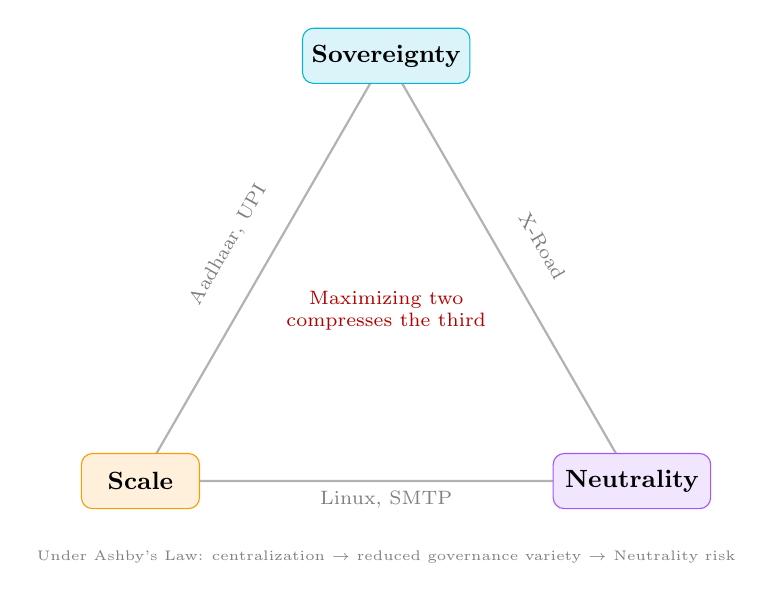
\begin{tikzpicture}[scale=1.2, font=\sffamily]
    % Triangle vertices
    \coordinate (S) at (0,3);      % Sovereignty (top)
    \coordinate (Sc) at (-2.6,-1.5);  % Scale (bottom left)
    \coordinate (N) at (2.6,-1.5);   % Neutrality (bottom right)

    % Draw triangle edges with labels
    \draw[thick, gray!60] (S) -- (Sc) -- (N) -- cycle;

    % Vertex labels with boxes
    \node[rectangle, rounded corners, draw=exitcolor, fill=exitcolor!15, minimum width=2cm, minimum height=0.7cm, font=\small\bfseries] at (S) {Sovereignty};
    \node[rectangle, rounded corners, draw=governcolor, fill=governcolor!15, minimum width=1.5cm, minimum height=0.7cm, font=\small\bfseries] at (Sc) {Scale};
    \node[rectangle, rounded corners, draw=auditcolor, fill=auditcolor!15, minimum width=2cm, minimum height=0.7cm, font=\small\bfseries] at (N) {Neutrality};

    % Edge labels showing what you get when you pick two
    \node[font=\scriptsize, text=gray, rotate=60, anchor=south] at (-1.5,0.9) {Aadhaar, UPI};
    \node[font=\scriptsize, text=gray, anchor=north] at (0,-1.5) {Linux, SMTP};
    \node[font=\scriptsize, text=gray, rotate=-60, anchor=south] at (1.5,0.9) {X-Road};

    % Center label
    \node[font=\scriptsize, text=red!70!black, align=center] at (0,0.3) {Maximizing two\\compresses the third};

    % Ashby annotation
    \node[font=\tiny, text=gray, align=center] at (0,-2.3) {Under Ashby's Law: centralization $\rightarrow$ reduced governance variety $\rightarrow$ Neutrality risk};
\end{tikzpicture}
\caption{\textbf{The Sovereignty, Scale, and Neutrality Tension.} Under centralized enforcement, states face structural pressure when optimizing for Sovereignty and Scale simultaneously. India Stack optimizes for Sovereignty + Scale with elevated Neutrality risk. Federated systems (Linux, SMTP) achieve Neutrality + Scale through distributed governance. X-Road holds Sovereignty + Neutrality at national rather than continental scale.}
\label{fig:trilemma}
\end{figure}

\textbf{Clarification: This Is Not an Impossibility Theorem.} The proposition does not assert that Sovereignty, Scale, and Neutrality are logically incompatible. It asserts that under centralized enforcement architecture, maximizing Sovereignty and Scale reduces governance variety unless compensatory mechanisms are introduced. The tension is architectural, not metaphysical. Neutrality can be preserved under Scale and Sovereignty if governance variety is restored through structural mechanisms such as federated execution, multi-issuer mandates, Functional Exit Equivalence (Section~\ref{subsubsec:fee}), state portability guarantees, or non-exclusive procurement rules.

India's experience instantiates this constraint: the architectural choices that achieved sovereign control and near-universal coverage produced structural dependency on a small set of switching and credentialing authorities. That dependency compressed the correction channel's bandwidth, manifesting as the GOVERN failures documented in Table~\ref{tab:govt_infra}. The tension reframes these outcomes: the observed compression of corrective bandwidth is not an implementation mistake but a predictable consequence of architectural choice.

\begin{table}[htbp]
\centering
\small
\caption{Comparative topology and neutrality risk}
\label{tab:topology-risk}
\begin{tabular}{lccc}
\toprule
\textbf{Topology} & \textbf{Sovereignty} & \textbf{Scale} & \textbf{Neutrality Risk} \\
\midrule
Centralized Sovereign Stack & High & High & Elevated \\
Federated Protocol Model & Medium & High & Lower \\
Market Platform Model & Low (State) & High & Variable \\
Open Commons Model & Low & Medium & Low \\
\bottomrule
\end{tabular}
\end{table}

Any prescriptive response must therefore treat neutrality as an architectural variable (portability, multi-issuer requirement, anti-exclusive procurement), not an aspirational outcome. The Functional Exit Equivalence remedies in Section~\ref{subsubsec:arch-responses} address precisely this constraint.

\subsection{The Essential Services Problem}
\label{subsec:essential}

A pattern emerges from the preceding analysis: systems that pass all five tests are disproportionately non-essential infrastructure. Linux, PostgreSQL, Kubernetes, and Let's Encrypt power critical operations, but no individual's survival depends on accessing them. The systems promoted as DPI, which mediate access to food, banking, healthcare, and mobility, consistently fail.

This correlation reflects a structural tension between essentiality and corrigibility.

\begin{proposition}[Essentiality-Corrigibility Tension]
\label{prop:essentiality}
For any infrastructure system $S$ where participation is a prerequisite to survival, the EXIT test cannot be satisfied by literal exit; verified Functional Exit Equivalence (Section~\ref{subsubsec:fee}) is the only remaining discharge path.
\end{proposition}

\begin{proof}
EXIT requires that refusal incur no disproportionate penalty (Section~\ref{sec:tests}, Test 1). Let $S$ be essential: participation is required for access to food, shelter, healthcare, or legal identity. Refusal of $S$ therefore entails exclusion from survival necessities. Exclusion from survival necessities is a disproportionate penalty by any reasonable standard. Therefore, EXIT fails. \qed
\end{proof}

This proposition formalizes the empirical observation: among the systems evaluated, those that pass all five tests are precisely those where participation remains genuinely voluntary.

\begin{corollary}[No Exemptions from Essentiality Tension]
The following do NOT constitute valid exemptions from Proposition~\ref{prop:essentiality}:
\begin{enumerate}[noitemsep]
    \item \textbf{Emergency necessity}: Pandemics, wars, and crises do not suspend the requirement for correction channels. Systems deployed under emergency conditions that block EXIT remain incorrigible; the emergency explains but does not justify the structural failure.
    \item \textbf{Efficiency gains}: That a mandatory system delivers services faster or cheaper than alternatives does not restore EXIT. Efficiency is orthogonal to corrigibility.
    \item \textbf{Democratic authorization}: Legislative mandates do not convert incorrigible systems into corrigible ones. A democratically enacted prison is still a prison.
    \item \textbf{Benevolent intent}: Good-faith operation does not substitute for structural accountability. The framework evaluates architecture, not intentions.
\end{enumerate}
\end{corollary}

\subsubsection{The Essentiality Trap}

Essential services create the economic coercion that undermines EXIT. When refusal means exclusion from survival, the feedback loop breaks regardless of other properties. \citet{hirschman1970} observed that exit is effective precisely because it is voluntary. The credible threat of departure disciplines the system. When departure means death (literal or social), exit ceases to function as feedback. It becomes self-exclusion.

The systems in Table~\ref{tab:positive} avoid this trap because alternatives exist. A developer who dislikes the Linux kernel's direction can migrate to BSD without losing the ability to compute. A journalist who distrusts Let's Encrypt can obtain certificates elsewhere. The existence of functional alternatives preserves the error signal.

Aadhaar has been made prerequisite to existence. Documented cases demonstrate the consequence: the Right to Food Campaign's tracking documented dozens of starvation deaths across Indian states between 2015 and 2018 --- by the campaign's own count, more than fifty, with a substantial share linked to Aadhaar-related exclusion from food rations \citep{rtfc2018,khera2017}. These deaths are not anomalies; they are the structural prediction of a system that blocks EXIT while governing essential services.

\subsubsection{Functional Exit Equivalence (FEE)}
\label{subsubsec:fee}

When an infrastructure is essential for survival, literal exit is impossible. However, the cybernetic purpose of EXIT is not departure itself; it is the generation of a credible error signal. Essential systems must therefore implement \textbf{Functional Exit Equivalence (FEE)}: architectural guarantees that recreate the error-signal strength of market exit without requiring citizens to abandon society.

FEE is achieved structurally through three combined mechanisms:
\begin{enumerate}[noitemsep]
    \item \textbf{Multi-Issuer Mandates:} Procurement requires at least two legally independent credential issuers (preventing single-point capture).
    \item \textbf{Acceptance Diversity:} Public services must accept federated credential classes, as demonstrated by the multi-national deployment of X-Road.
    \item \textbf{Protected Statutory Fallbacks:} The legal guarantee of non-digital analogues.
\end{enumerate}

The demand for FEE is not a regressive desire to maintain paper ledgers indefinitely; it is a rejection of algorithmic triage. \textbf{State capacity that achieves ``efficiency'' by mathematically guaranteeing that a non-zero percentage of the marginalized population will be incorrectly starved to death without recourse is not a public good.} The distributional stakes are taken up in Section~\ref{subsec:distributional}.

\begin{principle}[Functional Exit Equivalence]
An essential system $S$ satisfies FEE if compensatory architectural guarantees recreate error-signal strength comparable to market exit in non-essential systems. FEE is an engineered mechanism to maintain requisite variety in the controller when the natural market variety (EXIT) is suppressed. The formal operationalization appears in Appendix~\ref{appendix:proofs}.
\end{principle}

\paragraph{Operationalization.} FEE requires:
\begin{equation}
E_{\text{alt}} \geq \theta_E \times E_{\text{exit}}^{\text{baseline}}
\end{equation}
where $\theta_E$ is domain-specific (healthcare: 0.95; payments: 0.90; social benefits: 0.85). Example, using coverage as an auditable proxy for error-signal strength (the formal construct is defined in Appendix~\ref{appendix:proofs}, eq.~\ref{eq:error-signal}): if the Public Distribution System delivers food at $E_{\text{exit}}^{\text{baseline}} = 0.80$ proxy coverage, and $\theta_E = 0.85$ for social benefits, then any alternative must achieve $E_{\text{alt}} \geq 0.68$ to preserve functional exit. FEE operationalizes EXIT. Without it, ``opt-out'' is administrative theater.

\paragraph{Real-World Analogues.} A partial real-world analogue of Protected Alternatives can be observed in telecommunications number portability regimes and in Open Banking interoperability mandates (e.g., PSD2 in the European Union). These frameworks preserve service continuity while enabling institutional exit at the provider layer. While not fully satisfying EXIT in existential services such as identity, they demonstrate that architectural separation between infrastructure rails and service operators is technically feasible. Corrigibility does not demand regression to analog systems; it demands layered modularity that prevents existential lock-in.

\subsubsection{Design Responses to Proposition~\ref{prop:essentiality}}
\label{subsubsec:arch-responses}

The tension admits architectural resolutions that achieve FEE:

\paragraph{1. Protected Alternatives (Statutory Fallback).} Expanding the third FEE mechanism above: essential services can satisfy FEE if law guarantees functional non-digital equivalents. A model statutory clause:

\begin{quote}
\textit{``No person shall be required as a condition of receiving any essential public benefit to be exclusively dependent on a single digital system; the State shall maintain a legally enforceable analogue alternative and an interoperable credential acceptance guarantee.''}
\end{quote}

Cash preserves UPI's partial EXIT; eliminating cash would collapse UPI to Aadhaar's structural status. Corrigibility for essential services requires that non-digital pathways remain legally protected, not merely tolerated.

\paragraph{Bole Clause: Evidentiary Standard for Statutory Fallbacks.} A statutory fallback satisfies FEE only if it meets the Rule~A.9 evidentiary standard applied at the least-resourced stratum. Rule~A.9 requires: (i) a resolvable reference to the enabling instrument, (ii) its cryptographic hash, and (iii) historical evidence of enforcement. For statutory fallbacks the third requirement is operative availability at the margin: documented successful invocations of the analogue pathway by members of the least-resourced strata --- those with low digital literacy, remote location, missing biometric records, or administrative precarity --- within the audit window. A fallback legally guaranteed but practically inaccessible at the margin produces $E_{\text{alt}} \approx 0$ at the argmin stratum $x^*$ (Remark~\ref{rem:argmin}) regardless of its nominal coverage; it is operationally absent for exactly the population whose suppressed error signals the framework's central evidence (Section~\ref{sec:diagnosis}) documents. Design Response~5 (Funded Fallback Operations, Section~\ref{subsubsec:arch-responses} below) mitigates the gap but does not close it: funding is necessary; the test is operative availability at the margin, evidenced by invocation records.

The Bole Resolution of 1923 was a legislative guarantee of access to public water sources in the Bombay Presidency. It remained a dead letter for four years until collective action enforced it at Mahad, then required a further decade of litigation to survive the local order's counterattack. A statutory fallback is a GOVERN-class claim; GOVERN-class claims require enforcement history by the relevant subject class, not legislative text alone \citep{ambedkar1947states}.

\paragraph{2. Multi-Issuer Requirement.} Procurement and regulation shall require at least two legally independent credential issuers for each region or service class. No single issuer may be sole gatekeeper for eligibility. This creates credible switching alternatives that generate $E_{\text{alt}}$.

\paragraph{3. Credential Acceptance Diversity.} Expanding the second FEE mechanism above: public services must accept at least three credential classes (state, municipal, NGO/financial) to satisfy eligibility requirements. This prevents single-point-of-failure capture.

\paragraph{4. Binding Multi-Stakeholder Charter.} A legal instrument that locks governance rules, with amendments requiring supermajority approval, judicial review pathway, and defined emergency suspension conditions.

\paragraph{5. Funded Fallback Operations.} Government must fund and staff analogue fallback channels wherever the digital system is primary, not as legacy support but as structural accountability infrastructure.

\paragraph{Federated Implementation.} Rather than a single provider of essential infrastructure, services could be delivered through multiple independent implementations of open protocols. This is analogous to email (SMTP) rather than messaging (proprietary platforms).

Under this model, no single implementation would be essential; the protocol would be. A citizen excluded from one provider could obtain equivalent service from another. Estonian X-Road demonstrates this architecture (Section~\ref{sec:diagnosis}): passing CODE, AUDIT, GOVERN, and FORK while \emph{approaching} FEE through federated implementation. Its federation reduces concentration, but the citizen still cannot obtain the exchanged services through an alternative channel, so FEE is not verified and EXIT --- and with it the full determination --- remains failed. X-Road is the instructive near-miss, not a pass.

\subsubsection{The Finding}

The absence of fully corrigible essential services is not a limitation of this framework; it is the framework's central finding. The question ``Can essential DPI be fully corrigible?'' is answered: \textbf{not under architectures that eliminate alternatives, but achievable through designs whose FEE is verified} --- under Definition~\ref{def:exit}, verified FEE discharges EXIT, and a design that additionally passes the remaining four tests is fully corrigible. Proposition~\ref{prop:essentiality} is not a dead end; it is a design specification. No system evaluated in Section~\ref{sec:diagnosis} has yet met it.

\subsection{Why Incorrigibility Persists: The Choice of Architecture}
\label{subsec:architecture-choice}

The preceding subsections explain what incorrigibility does; they do not explain why governments choose it when corrigible alternatives exist. Four mechanisms sketch the answer; their formal development is future work (Section~\ref{sec:discussion}).

\begin{enumerate}[noitemsep]
    \item \textbf{Graded inequality as demand-side driver} \citep{ambedkar1936annihilation}. Every administrative rung gains standing over the rung below from an incorrigible stack; the coalition for correction fractures by design, because the people who bear the cost of incorrigibility are precisely those whose exit is most constrained and whose collective action is most structurally opposed.
    \item \textbf{Artifact openness as legitimacy cover.} Releasing code or weights under an open license satisfies the form of the commons claim while retaining governance closure; ``open DPI'' is the joint electorate at infrastructure scale \citep{ambedkar1945congress}: the form of inclusion, with power over the outcome retained by the operator.
    \item \textbf{Asymmetric legibility.} States have structural preferences for downward legibility, and corrigible designs by definition introduce upward channels that constrain administrative discretion; the information asymmetry that incorrigibility produces is often an intended feature, not an oversight.
    \item \textbf{Certification capture.} Openness properties (open license, open standard) are certified as if they were governance properties (collective choice, binding accountability), and the certification layer is captured by parties whose deployments it evaluates.
\end{enumerate}

Together these four mechanisms predict that incorrigibility is the default equilibrium in essential-services infrastructure, not a correctable anomaly --- which is why the framework treats correction capacity as an architectural precondition rather than an outcome the operator's incentives will eventually supply.

\section{Discussion}
\label{sec:discussion}

The political economy analysis above named the structural pressures that drive feedback-loop closure to fail. What remains is whether the binary determination holds under measurement uncertainty, whether the loop survives adversarial conditions, and what transition pathways remain open once a system is diagnosed as structurally incorrigible. This section takes them in turn: methodological foundations and the cybernetics of binary evaluation; corrigibility under adversarial conditions; and the political economy of accountability with its transition pathways, limits, and institutional preconditions.

\subsection{Methodological Foundations}
\label{subsec:methodology}

\subsubsection{The Cybernetics of Binary Evaluation}

Critics argue this framework's binary pass/fail topology is too rigid, proposing instead ``maturity models'' or graded scorecards. From a cybernetic perspective, we reject this gradation. Corrigibility is a \textbf{structural connectivity state}: a feedback loop is either closed or open. There is no ``mostly closed'' loop.

A system that allows \textbf{AUDIT} but blocks \textbf{GOVERN} is an \textbf{Open Loop}: it observes errors but cannot fix them. A system that allows \textbf{GOVERN} but blocks \textbf{EXIT} is a \textbf{Coercive Loop}: it traps correction demand, which accumulates until it discharges through channels the system cannot absorb. Figure~\ref{fig:failure_modes} contrasts these failure topologies against the closed-loop case. Partial compliance creates ``zombie infrastructure'': systems maintaining the aesthetic of responsiveness while severing actual stability capacity. A ``Partial'' score represents \textbf{Fatal Structural Failure}.

For diagnostic purposes, gradation remains useful. Tables~\ref{tab:operational-proxies-main} and~\ref{tab:three-indicator-main} specify continuous measurements. The binary determination is the output; continuous measurements are inputs. Evaluators can examine inputs to prioritize interventions.

\subsubsection{Legitimacy Threshold vs Physical Claim: A Two-Pronged Argument}
\label{subsubsec:two-pronged}

The binarity of corrigibility rests on two converging arguments that must be distinguished. Neither alone forces the conclusion; together they overdetermine it from independent grounds.

\paragraph{The Control-Theoretic (Mechanism) Argument.} Open-loop feedback yields divergent dynamics under persistent disturbance. Proposition~\ref{thm:null-feedback} formalizes this as a structural analogy. The mechanism claim is: when any feedback component is severed, the loop opens, and error accumulates without correction. Real systems exhibit continuous variation in loop gain, observability, and actuation authority --- a sensor with 50\% accuracy transmits \textit{some} signal --- so the mechanism argument alone yields divergence-rate claims, not legitimacy claims.

\paragraph{The Political-Theoretic (Legitimacy) Argument.} Partial contestation creates \textit{sham governance}: cosmetic accountability without corrective leverage. A system that admits 10\% of grievances, or that admits all grievances but resolves them only after harm has accumulated past reversibility, is institutionally distinct from a system with no contestation only in appearance. Beyond a threshold of feedback quality, additional gradations in compliance produce \textit{non-monotonic} legitimacy gains: increases in nominal contestation procedures may decrease real correction capacity by absorbing political pressure into procedure rather than outcome. Below this threshold, a system forfeits the right to claim public legitimacy under any non-domination criterion (Section~\ref{sec:theory}, Normative Anchor). The threshold is binary because legitimacy is binary: a prison that permits appeals 10\% of the time is still a prison.

\paragraph{Why Both Arguments Are Needed.} The control-theoretic argument tells us that partial corrigibility cannot stabilize a system; the political-theoretic argument tells us that partial corrigibility cannot legitimize one. The conjunction yields the framework's binarity claim. Critics who reject the political-theoretic grounding can still accept the mechanism conclusion; critics who reject the control-theoretic abstraction can still accept the legitimacy conclusion. The framework is robust to either critique because it does not depend on either argument alone.

\paragraph{Sensitivity Analysis.} Let continuous inputs be $\{p, v, m, g, r\}$ --- penalty ratio, visibility fraction, mean time to detect (MTTD), governance bindingness-and-throughput, and fork resource ratio --- the per-test proxies of Table~\ref{tab:operational-proxies-main}. The binary determination function $D$ is:

\begin{equation}
D = \mathbf{1}[p \leq p^*] \land \mathbf{1}[v \geq v^*] \land \mathbf{1}[m \leq m^*] \land \mathbf{1}[g = \text{binding}] \land \mathbf{1}[r \leq r^*]
\end{equation}

where $\mathbf{1}[\cdot]$ is the indicator function and $\{p^*, v^*, m^*, r^*\}$ are threshold values. (The symbol $\tau$ is reserved for governance throughput in Table~\ref{tab:operational-proxies-main}; the AUDIT latency proxy is written $m$ here to avoid collision.) This formulation makes explicit that:
\begin{enumerate}[noitemsep]
    \item Continuous inputs are preserved for diagnosis
    \item The AND-conjunction enforces the ``weakest link'' principle
    \item Threshold calibration is a policy choice, separable from the structural argument
\end{enumerate}

Systems near thresholds warrant scrutiny; systems far below thresholds across multiple dimensions are unambiguously incorrigible. The binary output serves regulatory clarity; the continuous inputs serve diagnostic priority.

\subsubsection{Continuous Indicators for Diagnostic Use}

The continuous measurements underlying binary determinations enable both threshold calibration and diagnostic prioritization. Table~\ref{tab:operational-proxies-main} specifies operational proxies; Table~\ref{tab:three-indicator-main} formalizes the three-indicator protocol.

\begin{table}[htbp]
\centering
\caption{Operational proxies for the five tests. Thresholds are illustrative and subject to calibration.}
\label{tab:operational-proxies-main}
\begin{tabular}{lll}
\toprule
\textbf{Test} & \textbf{Proxy Metric} & \textbf{Illustrative Threshold} \\
\midrule
EXIT & Penalty ratio $p$ & $p \leq 1.2$ \\
CODE & Visibility fraction $v$ & $v \geq 0.9$ \\
AUDIT & Mean time to detect (MTTD) & MTTD $\leq$ 24 hours \\
GOVERN & Bindingness + throughput $\tau$ & binding = true, $\tau \geq 1$ per 10k users/day \\
FORK & Resource feasibility ratio $r$ & $r \leq 10^{-3}$ \\
\bottomrule
\end{tabular}
\end{table}

\textbf{Interpretation:} Penalty ratio $p$ = cost(non-digital alternative) / cost(digital). Visibility $v$ = public LOC / total LOC on critical execution path. Resource ratio $r$ = estimated FLOP to retrain / aggregate community compute capacity.

\begin{table}[htbp]
\centering
\scriptsize
\caption{Three-indicator protocol: continuous score, binary flag, and threshold metric for each test. Table~\ref{tab:operational-proxies-main} gives the screening-tier proxies; this protocol adds the binary flags and evidence metrics used at certification.}
\label{tab:three-indicator-main}
\begin{tabular}{@{}lp{2.8cm}p{2.8cm}p{3.2cm}@{}}
\toprule
\textbf{Test} & \textbf{Continuous} & \textbf{Binary} & \textbf{Threshold} \\
\midrule
EXIT & \texttt{penalty\_ratio}: exit cost / stay cost & \texttt{legal\_barrier}: criminalized? & $p \leq 1.2$ AND barrier = false \\
CODE & \texttt{visibility}: public LOC / critical path LOC & \texttt{build\_repro}: deterministic build? & $v \geq 0.95$ AND build = true \\
AUDIT & \texttt{observability}: \% verifiable transactions & \texttt{access}: third parties test? & $o \geq 0.9$ AND access = true \\
GOVERN & \texttt{override\_rate}: operator overrule rate & \texttt{charter}: irrevocable instrument? & $r = 0$ AND charter = true \\
FORK & \texttt{cost\_ratio}: fork / community resources & \texttt{rights}: fork-permitting license? & $c \leq 0.001$ AND rights = true \\
\bottomrule
\end{tabular}
\end{table}

\paragraph{Inter-Rater Calibration.} Before deployment, independent auditors should assess 3--5 systems using this protocol and compare determinations. Disagreements identify threshold calibration issues. Target: $\kappa \geq 0.8$ (Cohen's kappa) for binary determinations.

\paragraph{Policy Constants Summary.} The framework employs several calibration constants that represent policy choices separable from the structural argument. Table~\ref{tab:policy-constants} consolidates these for reference. The constants are policy choices, not engineering discoveries. Every threshold creates an operator interest in where it is set, so calibration must itself satisfy a deliberative-mechanism condition (affected-class participation, documented rationale, periodic external review), for the same structural reason that GOVERN cannot be operator self-certification (Section~\ref{subsec:limitations}).

\begin{table}[htbp]
\centering
\small
\caption{Policy constants used throughout the framework. Values are recommended defaults and calibration starting points, separable from the structural argument. Per-test pass/fail thresholds are listed in Tables~\ref{tab:operational-proxies-main} and~\ref{tab:three-indicator-main}.}
\label{tab:policy-constants}
\begin{tabular}{@{}llll@{}}
\toprule
\textbf{Symbol} & \textbf{Name} & \textbf{Range} & \textbf{Section} \\
\midrule
$\tau_{\text{exit}}$ & Exit-penalty material-exclusion threshold & Context-dependent & \ref{sec:tests} \\
$\theta_E$ & FEE sufficiency threshold & $0.8$--$1.0$ & \ref{subsubsec:fee} \\
$\Sigma^*$ & Portability threshold (EXIT/FORK failure) & 2.0 on the normalized $[0,5]$ scale & \ref{appendix:proofs} \\
$\kappa$ (Cohen) & Inter-rater agreement target (Cohen's kappa) & $\geq 0.8$ & \ref{subsec:methodology} \\
$\theta$ & Neutrality stability threshold & $(0, 1]$ & \ref{appendix:neutrality} \\
$Sc^*$ & Scale threshold for neutrality degradation & Context-dependent & \ref{appendix:neutrality} \\
$\alpha^*$ & Fork adoption critical mass & $0.3$--$0.5$ & schema repo \\
$\epsilon$ & Correction friction cost & Context-dependent & \ref{appendix:proofs} \\
\bottomrule
\end{tabular}
\end{table}

\begin{figure}[htbp]
\centering
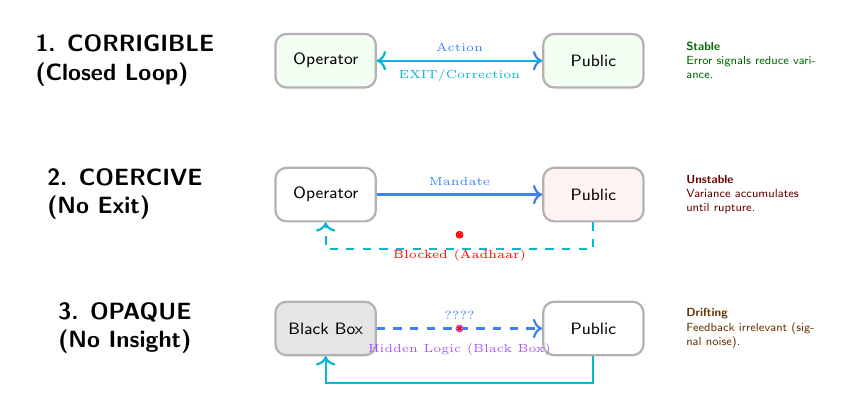
\begin{tikzpicture}[
    scale=0.85, transform shape,
    box/.style={rectangle, draw=gray!60, thick, fill=white, rounded corners, minimum height=0.8cm, minimum width=1.5cm, font=\scriptsize\sffamily},
    lbl/.style={font=\tiny\sffamily\bfseries, color=gray},
    cross/.style={path picture={
        \draw[red, thick] (path picture bounding box.south west) -- (path picture bounding box.north east);
        \draw[red, thick] (path picture bounding box.south east) -- (path picture bounding box.north west);
    }}
]

% -- ROW 1: CORRIGIBLE (Closed Loop) --
\node[font=\bfseries\sffamily, align=left] at (-3, 0) {1. CORRIGIBLE\\(Closed Loop)};
\node[box, fill=green!5] (op1) at (0,0) {Operator};
\node[box, fill=green!5] (us1) at (4,0) {Public};

\draw[->, thick, codecolor] (op1) -- node[above, font=\tiny] {Action} (us1);
\draw[->, thick, exitcolor] (us1) -- node[below, font=\tiny] {EXIT/Correction} (op1);

\node[right=0.5cm of us1, font=\tiny\sffamily, text width=2cm, align=left, color=green!40!black] {
    \textbf{Stable}\\
    Error signals reduce variance.
};

% -- ROW 2: COERCIVE (No Exit) --
\node[font=\bfseries\sffamily, align=left] at (-3, -2) {2. COERCIVE\\(No Exit)};
\node[box] (op2) at (0,-2) {Operator};
\node[box, fill=red!5] (us2) at (4,-2) {Public};

\draw[->, thick, codecolor] (op2) -- node[above, font=\tiny] {Mandate} (us2);
\draw[->, thick, exitcolor, dashed] (us2.south) -- +(0,-0.4) -| (op2.south);
\node[circle, fill=white, draw=red, inner sep=1pt, cross] at (2, -2.6) {};
\node[below, font=\tiny, color=red] at (2, -2.7) {Blocked (Aadhaar)};

\node[right=0.5cm of us2, font=\tiny\sffamily, text width=2cm, align=left, color=red!40!black] {
    \textbf{Unstable}\\
    Variance accumulates until rupture.
};

% -- ROW 3: OPAQUE (No Inspection) --
\node[font=\bfseries\sffamily, align=left] at (-3, -4) {3. OPAQUE\\(No Insight)};
\node[box, fill=gray!20] (op3) at (0,-4) {Black Box};
\node[box] (us3) at (4,-4) {Public};

\draw[->, thick, codecolor, dashed] (op3) -- node[above, font=\tiny] {????} (us3);
\node[circle, fill=white, draw=auditcolor, inner sep=1pt, cross] at (2, -4) {};
\node[below, font=\tiny, color=auditcolor] at (2, -4.1) {Hidden Logic (Black Box)};

\draw[->, thick, exitcolor] (us3.south) -- +(0,-0.4) -| (op3.south);

\node[right=0.5cm of us3, font=\tiny\sffamily, text width=2cm, align=left, color=orange!40!black] {
    \textbf{Drifting}\\
    Feedback irrelevant (signal noise).
};

\end{tikzpicture}
\caption{\textbf{Topologies of Failure.}
(1) A corrigible system closes the loop, converting error signals into stability.
(2) A coercive system blocks \textbf{EXIT}, trapping energy.
(3) An opaque system obscures the action channel, making feedback unintelligible.}
\label{fig:failure_modes}
\end{figure}

\subsection{Corrigibility Under Adversarial Conditions}
\label{subsec:adversarial}

A frequent objection to structural transparency requirements (EXIT, CODE, AUDIT, GOVERN, FORK) concerns adversarial security environments. Critics argue that permitting external audit or interoperability in critical digital infrastructure (particularly identity, payments, or routing rails) may expand the attack surface available to hostile states or organized cyber actors.

This framework does not equate corrigibility with unrestricted public exposure of live exploit vectors. Corrigibility requires \textbf{structured contestability}, not indiscriminate disclosure. The distinction is architectural:

\begin{itemize}[noitemsep]
    \item \textbf{Auditability} refers to verifiable oversight mechanisms (cryptographic proofs, independent inspection rights, reproducible builds, sandboxed red-teaming, hardware-isolated verification environments), not public release of zero-day vulnerabilities.
    \item \textbf{CODE transparency} requires inspectability of system logic and ontology, but does not mandate real-time publication of operational secrets (e.g., private keys, network topologies, live intrusion telemetry).
    \item \textbf{GOVERN mechanisms} may incorporate tiered access controls and certified verifiers, provided the certification process itself remains contestable.
\end{itemize}

Security and corrigibility are not mutually exclusive variables; rather, both depend on layered design. In adversarial contexts, excessive opacity can itself become a systemic vulnerability by preventing early detection of latent design flaws. Historical failures in both public and private infrastructure demonstrate that closed architectures do not eliminate breach risk; they merely concentrate it.

Accordingly, the framework assumes:
\begin{enumerate}[noitemsep]
    \item Security controls may limit raw exploit exposure.
    \item Such controls must not eliminate independent verification pathways.
    \item Emergency override or classified layers must themselves be subject to post-hoc audit.
\end{enumerate}

Corrigibility in adversarial environments therefore implies \textbf{structured verifiability}, not universal visibility. The objective is to preserve corrective bandwidth without compromising defensive posture.

\subsection{Political Economy of Accountability}
\label{subsec:political-economy-discussion}

\subsubsection{The Protocol Model of State}

A common practical objection holds that governments cannot adopt corrigible infrastructure because they must retain control over sovereign functions. This objection relies on a category error: it conflates the \textit{Platform Model} with the \textit{Protocol Model}.

In the \textbf{Platform Model} (currently dominant), the state contracts a vendor to build a monolithic silo (e.g., existing digital ID systems). The vendor controls execution, the state attempts to control policy, and citizens are reduced to rows in a database. As \citet{cohen2019} argues, this model inevitably subverts the Rule of Law by replacing legal due process with optimized platform logic. In the \textbf{Protocol Model} (the corrigible alternative), the state adopts open, corrigible protocols and acts as a high-authority participant within them. The state issues credentials and verifies claims, but it does not enclose the infrastructure itself.

This distinction mirrors the architecture of the web. Governments do not need to build their own proprietary browsers to deliver services; they build sites on HTTP. Similarly, corrigible DPI implies that the state becomes an issuer of trust rather than a landlord of infrastructure. This model does not reduce state capacity; it enhances trust by making the state's operations verifiable.

\subsubsection{Distributed Assessment Capacity}
A corollary objection concerns resources: ``Who audits?'' The framework does not require every citizen to audit source code. It requires that the infrastructure allows \textit{anyone} to audit, thereby enabling civil society, journalists, and specialized firms to perform this function on behalf of the public. Assessment capacity is itself infrastructure. When systems are designed to be inscrutable, this immune system of society withers.

\subsection{Corrigibility in Extremis}

Incorrigibility is often justified by the rhetoric of necessity, such as national security, anti-corruption, or emergency efficiency. This framework explicitly denies such exemptions. Corrigibility does not imply that substantive rules are negotiable; a system may enforce strict, non-negotiable limits (e.g., pandemic travel restrictions or environmental caps). However, the \textit{structural capacity} to detect error, verify correct enforcement, and reverse wrongful harm must remain intact even in high-constraint environments. As safety engineering demonstrates, accidents in complex systems are caused precisely by the lack of appropriate constraints on component interactions \citep{leveson2011}.

\begin{claim}[No Structural Exemption]
\label{claim:no-exemption}
No exemption from the five tests is granted on the basis of emergency conditions, planetary constraints, or decentralized architecture.
\end{claim}

This applies equally to decentralized systems. Cryptographic immutability is not a substitute for governance. A blockchain that permanently records a theft without a mechanism for consensus-based reversion is not ``trustless''; it is strictly incorrigible. If a system allows for irrevocable harm without recourse, its decentralization is merely a distribution of unaccountability.

\subsubsection{Political vs Structural Corrigibility}
\label{subsec:political-structural}

A critical objection holds that the framework applies market logic (exit/fork) to non-market systems. You cannot fork India.

The response requires distinguishing two modes of correction:

\begin{itemize}
    \item \textbf{Political corrigibility} (voice via elections): how \textit{states} are corrected
    \item \textbf{Structural corrigibility} (exit/fork): how \textit{infrastructure} is corrected
\end{itemize}

States are corrected politically. DPI sits \textit{below} politics; that is the structural crisis. When DPI is captured by executive authority or vendor monopolies, political correction mechanisms do not reach it. \textbf{Aadhaar operated for seven years under executive fiat before receiving parliamentary authorization as a money bill (2009--2016)} \citep{bhatia2019}.

This is not a hypothetical concern. It is the documented history of the system most frequently cited as a DPI success story. The gap the framework identifies is infrastructure that escapes democratic correction entirely.

Shifting to the \textbf{Protocol Model of State}, where the government acts as an issuer of trust on an open standard rather than a landlord of a private platform, does not surrender sovereignty to technocrats. It returns sovereignty to the legislature, because open protocols cannot be unilaterally weaponized by the executive branch. The Constitution can be amended through democratic process; Aadhaar's architecture cannot be voted on.

\subsubsection{The Distributional Question}
\label{subsec:distributional}

The debate is not ``scale vs sovereignty.'' The debate is \textbf{whose suffering counts}.

\begin{itemize}
    \item Platform speed benefits the median user.
    \item Incorrigibility harms the marginal user.
    \item The marginal user has no voice because EXIT is blocked.
\end{itemize}

Corrigibility is a \textbf{distributional question}. The framework makes visible who bears the cost of system failures. When we ask ``Is this system corrigible?'' we are really asking: ``When this system fails someone, can they do anything about it?''

The answer for Aadhaar is no. Documented starvation deaths in Jharkhand were not caused by ``too much democracy''; they were caused by a system where the marginal user had no recourse when biometric authentication failed.

\subsection{Pathways and Limits}
\label{subsec:pathways}

\subsubsection{Transition Paths}
\label{subsec:transition}

The framework diagnoses incorrigibility but does not prescribe political remedies. However, the structure of the five tests implies an ordering for transition: certain tests are prerequisites for others, and certain interventions have higher leverage.

\subsubsection{Ordered Priorities}

The tests form a dependency chain when considered as a transition sequence:

\begin{enumerate}
    \item \textbf{EXIT first.} Restore exit before other tests. Without exit, no other reform creates genuine feedback. This requires either eliminating mandatory linkage laws or guaranteeing functional non-digital alternatives. EXIT is the error signal; without it, the system cannot sense its own failures.

    \item \textbf{CODE before AUDIT.} Transparency must precede verification. Independent testing is meaningful only if the testing target is observable. Publishing audit results for a black box proves nothing about the box.

    \item \textbf{AUDIT before GOVERN.} Verified error data creates political pressure for governance reform. Governance without measurement is arbitrary. There is no basis for determining whether constraints are adequate. The sensor must function before the actuator can be calibrated.

    \item \textbf{GOVERN enables FORK.} Structural governance can mandate open licensing, data portability, and interoperability requirements that enable eventual forkability. GOVERN without FORK leaves the system captive to its current steward; FORK without GOVERN may produce fragmentation without accountability.
\end{enumerate}

This sequence reflects the causal structure of the feedback loop: signal, sensing, transmission, actuation, selection. Interventions at later stages are ineffective if earlier stages are broken.

\subsubsection{Phase Transitions}

The transition is not gradual improvement. It is a series of phase transitions. Each test either passes or fails; the system remains incorrigible until all five pass. A system that achieves CODE but not EXIT has become transparent without becoming accountable. Users can observe the system's logic but cannot modify their participation.

This explains why open-washing is effective: partial progress creates the appearance of reform while preserving structural capture. The framework rejects partial credit precisely because partial feedback loops do not partially function.

\subsubsection{Political Economy}

The political economy of transition varies by test, with each barrier facing a characteristically different concentrated opposition (Table~\ref{tab:political-economy}):

\begin{table}[h]
\centering
\caption{Political economy of transition by test}
\label{tab:political-economy}
\begin{tabular}{lll}
\hline
\textbf{Test} & \textbf{Transition Barrier} & \textbf{Concentrated Opposition} \\
\hline
EXIT & Mandatory linkage laws & Operators lose captive users \\
CODE & Intellectual property claims & Vendors lose competitive moats \\
AUDIT & Security-through-obscurity claims & Operators lose narrative control \\
GOVERN & Sovereignty objections & Executives lose discretion \\
FORK & Typically least opposed & Requires only licensing and documentation \\
\hline
\end{tabular}
\end{table}

FORK is typically the least opposed transition because it requires only legal permission and technical documentation. It does not immediately threaten operator control. However, FORK without the prior four tests is meaningless: the right to reproduce a system you cannot inspect, verify, govern, or exit provides no actual power.

\subsubsection{Cost Considerations}

Transition is not costless. The European Commission \citep{eu2021oss} estimated that public sector open-source adoption yields cost-benefit ratios above 1:4, but this ratio assumes successful implementation. Transition costs include personnel retraining, system compatibility engineering, procurement policy updates, and organizational change.

However, these costs must be weighed against the costs of continued incorrigibility:

\begin{itemize}
    \item Litigation costs from unresolvable grievances
    \item Political instability from suppressed correction demand (Section~\ref{subsec:velocity})
    \item Technical debt from opacity-enabled shortcuts
    \item Vendor lock-in premiums from non-forkable dependencies
    \item Human costs: documented deaths, exclusions, and deprivations
\end{itemize}

The systems in Table~\ref{tab:positive} demonstrate that corrigibility at scale is economically sustainable. Linux, Kubernetes, and Let's Encrypt operate at population scale with resource models that have proven durable over decades.

\subsubsection{Coordination Goods and Inherent Unforkability}
\label{subsec:coordination}

The forking paradox presents a genuine limitation: if you can fork the Public Infrastructure, it may no longer be public.

A ``public'' good (like law or money) derives its value from universality. We all agree on the same truth. If the Identity System is ``forkable,'' and I fork it to create ``Blue-Identity'' while you use ``Red-Identity,'' we have destroyed the common knowledge required for society to function.

\begin{remark}[Latent Forkability in Coordination Goods]
Identity, money, and law are coordination goods; their value derives from uniqueness. If the exercise of FORK destroys the society's ability to coordinate, it functions as mutually assured destruction.

The framework resolves this through \textbf{Latent Forkability} --- the equilibrium the Credible Replaceability remark (Section~\ref{sec:tests}) already established: the credible threat of reproduction disciplines the center without requiring routine divergence. What the coordination-goods case adds is the stake: where the good's value derives from uniqueness, the exercised fork functions as mutually assured destruction, so the threat must remain latent to remain usable. The framework penalizes \textit{constructed legal barriers} to reproduction, not the \textit{natural economic friction} of network effects.
\end{remark}

Whether this equilibrium is achievable for identity infrastructure remains an open question, but the existence of federated identity systems (X-Road, Matrix, AT Protocol) demonstrates that latent forkability is technically achievable even for coordination-sensitive infrastructure.

\subsubsection{Engaging ``Regulate the Loop''}
\label{subsec:regulate}

A sophisticated objection accepts the diagnosis but rejects the prescription:

\begin{quote}
``We accept your Diagnosis (The Loop is Broken). We reject your Prescription (Break the Platform). We choose to \textbf{Regulate the Loop} rather than Fork the Code, because the cost of Forking is Poverty.''
\end{quote}

This argument has force. UPI moved from zero to over 20 billion monthly transactions within a decade of launch \citep{npci2026}. Email standardization took decades. India does not have decades. Poverty is now.

\textbf{Where this lands:}
\begin{itemize}
    \item RBI \textit{could} mandate error rate disclosure, demographic audits, grievance SLOs
    \item Political correction (parliament, courts) exists even without FORK
    \item Speed-to-scale tradeoff is real
\end{itemize}

\textbf{Where this misses:}
\begin{itemize}
    \item ``Regulate the loop'' assumes trustworthy regulators. RBI reports to the Finance Ministry. UIDAI operated for seven years on executive notification alone, and even post-statute combines operator and regulator roles with oversight limited to post-hoc CAG audit. Who regulates the regulator?
    \item In captured states, ``regulate later'' means ``never''
    \item Gmail $\neq$ UPI: Gmail \textit{earned} users with features: you CAN leave for Proton, Fastmail, self-hosted. UPI has \textit{regulatory monopoly}: you CANNOT build a competing instant payment switch. Absent structural alternatives, Gmail's correction depends on market choice; UPI's correction depends on regulatory discretion.
    \item ``Regulate later'' rarely happens: Aadhaar 2009 pilot $\rightarrow$ 2016 mandatory $\rightarrow$ 2018 Supreme Court $\rightarrow$ still no real audit. 15 years. Where's the regulation?
\end{itemize}

This tension is not hypothetical. A documented debate between advocates of open standards (arguing for specification transparency and independent security audits) and proponents of centralized control (arguing that controlled governance enables ``faster iteration'') reveals the core disagreement \citep{abraham2020}. The efficiency argument is genuine; but efficiency without accountability is capture dressed as service.

\subsection{Utility Does Not Equal Accountability}
\label{subsec:utility}

A system can be \textbf{useful AND structurally captured}. Both are true simultaneously.

UPI \textit{has} democratized payments. The framework risks dismissing real-world impact if this is not acknowledged. But the question the framework asks is different: \textbf{When UPI fails someone, can they correct it?}

The answer is no. This is the point.

The framework measures \textbf{accountability structure}, not \textbf{utility}. A system can score 0/5 and still be beneficial. The score indicates \textit{structural risk}, not \textit{current harm}. A house built without fire exits can function perfectly for decades, until there is a fire.

\subsection{Institutional Preconditions for Large-Scale Corrigibility}
\label{subsec:institutional}

The framework presumes the existence of intermediary institutions capable of exercising audit, representation, and governance functions. At population scales involving tens or hundreds of millions, spontaneous civic coordination cannot be assumed.

Unlike open-source software communities, where contributors are self-selected and technically specialized, state-scale infrastructure must serve heterogeneous populations with asymmetric digital literacy, resource access, and organizational capacity. The structural availability of audit rights does not guarantee their effective exercise.

Accordingly, structural corrigibility requires:

\begin{description}[noitemsep]
    \item[Independent Verification Bodies] Publicly funded or legally mandated audit institutions insulated from operator control.
    \item[Civic Technical Intermediaries] NGOs, academic labs, and watchdog entities with standing to invoke GOVERN mechanisms.
    \item[Distributed Representation Channels] Mechanisms allowing affected groups to escalate systematic errors collectively, rather than solely through individual grievance.
    \item[Anti-Capture Safeguards] Rotation requirements, transparency obligations for auditors, and conflict-of-interest constraints to prevent elite capture of oversight functions.
\end{description}

The framework does not assume idealized commons governance. It asserts instead that without institutionalized intermediaries, formal corrigibility tests degrade into symbolic compliance.

In this sense, \textbf{corrigibility is necessary but not sufficient for equitable outcomes}. Institutional capacity determines whether structural safeguards translate into practical accountability.

\section{Conclusion and Transition Paths}

Digital Public Infrastructure is a claim of political legitimacy. Such legitimacy cannot be derived from self-declarations, ``open standards'' labeling, or multilateral endorsements. It requires \textbf{Corrigibility}: the capacity of the governed to observe the rules, verify their execution, limit their reach, and reproduce the infrastructure to escape its capture.

Five architectural constraints verify this capacity. The analysis demonstrates that systems currently touted as DPI models (Aadhaar, UPI) fail these tests, revealing them to be administrative enclosures rather than public goods. Conversely, the systems which actually run the world (Linux, Kubernetes, Let's Encrypt) pass them structurally.

\subsection{The Roadmap Out}

The structure of the five tests implies an ordering for transition (detailed in Section~\ref{subsec:pathways}): EXIT $\to$ CODE $\to$ AUDIT $\to$ GOVERN $\to$ FORK. This sequence reflects the causal structure of the feedback loop. Interventions at later stages are ineffective if earlier stages are broken.

\subsection{The Core Finding}

The choice is not between chaos and control. It is between \textbf{Open Loop} systems that drift toward fragility and authoritarianism, and \textbf{Closed Loop} systems that stabilize themselves through the correction of those they serve.

\begin{quote}
\textit{Systems that cannot be corrected by those they affect will eventually be corrected by forces they cannot control.}
\end{quote}

\subsection{Summary of Topological Risk}

The ``physics'' of digital governance demonstrates that certain architectures structurally increase the risk of capture independent of operator intent. The transition to platform-mediated governance does not eliminate the need for the Rule of Law; it necessitates its translation into the \textbf{Rule of the Ledger} (Section~\ref{subsec:rule-of-ledger}) --- and, in the agentic setting the companion paper takes up, the Rule of the Workflow~\citep{aravind2026epi}. Table~\ref{tab:topological-risk} maps the principal failure modes and structural remedies across identity, payment, and data-exchange layers.

\begin{table}[htbp]
\centering
\caption{Failure modes and structural remedies by infrastructure layer}
\label{tab:topological-risk}
\begin{tabular}{llll}
\toprule
\textbf{Layer} & \textbf{Primary Failure Mode} & \textbf{Capture Type} & \textbf{Structural Remedy} \\
\midrule
Identity & Dependency & Administrative & FEE / Portability \\
Payment & Lock-In & Transactional & Multi-Rail / Interoperability \\
Data Exchange & Siloing & Coordination & Open Standards / APIs \\
\bottomrule
\end{tabular}
\end{table}

Corrigibility is the structural response to the Collingridge Dilemma (Section~\ref{subsec:velocity}): architectural constraints must be established before entrenchment makes correction impossible.

\subsection{Limitations}
\label{subsec:limitations}

\begin{enumerate}
    \item \textbf{Methodological scope: binary determinations.} The binary determination answers ``Does this system merit the claim of public infrastructure?'' rather than ``Which constraint should reformers address first?''; the continuous metrics in Tables~\ref{tab:operational-proxies-main} and~\ref{tab:three-indicator-main} serve diagnostic prioritization, while the binary output serves the legitimacy threshold. The control-theoretic formalization (Proposition~\ref{thm:null-feedback}) is labeled in-text as a structural analogy rather than a predictive dynamics claim, and the framework evaluates legitimacy rather than stability: incorrigible systems may persist indefinitely without being legitimate.

    \item \textbf{Solution validation gaps: FORK, FEE, and prescriptive limits.} FORK may be structurally unachievable for essential state infrastructure: legal monopoly, network effects, data non-portability, and decade-long trust bootstrapping are barriers technical openness alone cannot overcome, and the framework provides no demonstrated example of essential state identity infrastructure disciplined by an actually executed fork. Functional Exit Equivalence (FEE) is proposed as the resolution for the essentiality-corrigibility tension, but no essential identity infrastructure has implemented full FEE; partial analogues (telecom number portability, PSD2 banking APIs) operate in domains with weaker network effects. The framework is therefore primarily diagnostic; the prescriptive elements (FEE, open licensing, multi-stakeholder governance) remain theoretical constructs requiring empirical validation.

    \item \textbf{Evaluation interpretive limits.} GOVERN requires historical evidence of enforcement and is therefore more interpretation-dependent than the technical tests. The correction-velocity critique targets external bureaucracies (courts, ombudsmen) rather than all deliberative processes; Bitcoin's BIP process and other community-paced governance remain valid governance under the framework.

    \item \textbf{Network effects are not formally modeled.} Network effects can make formally forkable systems practically unforkable (e.g., Signal's open code but unfederated network). The framework treats this as natural economic friction rather than constructed legal barrier, but does not provide a quantitative model for when network friction crosses into capture.

    \item \textbf{Empirical scope limitations.} The primary case studies (Aadhaar, UPI) derive from India Stack; Pix and X-Road receive five-test evaluations in Section~\ref{sec:diagnosis}, but systematic validation across further national DPI implementations (Singapore NDI, Kenya M-Pesa, the EU Digital Identity Wallet) is required before universal claims are established. The political economy of why governments choose incorrigible designs is sketched as four mechanisms in Section~\ref{subsec:architecture-choice}; its formal development remains future work.

    \item \textbf{The framework encodes specific values.} This framework prioritizes structural accountability through exit mechanisms (the capacity to leave or reproduce) over voice mechanisms (political participation, democratic oversight), reflecting a specific intellectual tradition (Hirschman's exit/voice distinction, Stallman's free software principles, commons governance theory). Alternative frameworks prioritizing voice have independent value. The framework is not ideologically neutral; it makes explicit what it values.
\end{enumerate}

\subsection{Future Work}

Extensions warranting investigation: (1) \textbf{Empirical velocity measurement}, quantifying when systems become ungovernable; (2) \textbf{International comparison}, testing generality across X-Road, Singapore NDI, EU Digital Identity, Brazil Pix; (3) \textbf{Political economy of architecture choice}, developing formally the four mechanisms sketched in Section~\ref{subsec:architecture-choice}; (4) \textbf{Transition cost modeling}; (5) \textbf{Legal doctrine integration}, operationalizing corrigibility for courts; (6) \textbf{Network effect formalization}; (7) \textbf{FEE pilot design}, specifying implementable FEE mechanisms for identity infrastructure. A companion paper~\citep{aravind2026epi} extends this framework to learned systems (AI/ML) where behavior is determined by training data rather than source code.

\paragraph{Liability and Enforcement.} Architectural corrigibility must be complemented by clear liability and enforcement semantics: for any failure mode, this framework's supply-chain roles (principal, integrator, operator, trustee) must be mappable onto the value-chain roles the law actually distinguishes --- provider, deployer, importer, distributor, authorised representative under the EU AI Act \citep{euaiact2024} --- and to mandated mitigation steps, so that evidence produces enforceable consequences rather than forensic narrative alone.

\paragraph{Adversarial Robustness.} This framework assumes good-faith actors operating within institutional constraints. It does not address adversarial manipulation: coordinated gaming of audit mechanisms, governance capture through procedural compliance, or fork-and-poison attacks. Extension to adversarial settings requires additional machinery beyond this paper's scope.

\paragraph{Methodological Note.} The five-test structure presented here did not emerge from theoretical deduction; it hardened across successive revisions through adversarial engagement with live systems. Each version closed a specific loophole: self-attestation gave way to independent assessment; partial-credit ``maturity models'' gave way to strict binary determination; advisory governance was disqualified in favor of non-overrideable constraint; substitution (EXIT) was distinguished from reproduction (FORK); and decentralized identifiers were prevented from laundering centralized governance via layer-decomposed evaluation. The framework's audit trail---version history, schema changelogs, and the rules that govern protocol revision---is maintained in the schema repository.

\subsection*{Core Thesis}
Corrigibility defines the boundary between reversible and irreversible infrastructure. It does not guarantee justice. It does not optimize administration. It guarantees that corrective authority remains structurally available to those the system governs. Digital infrastructure aspires to durability. Corrigibility ensures durability does not become capture. Public systems are either structurally reversible or structurally irreversible. Corrigibility marks that boundary.

\section*{Acknowledgments}

This work draws on the author's lived practice across the three traditions it triangulates: two decades of free-software contribution and engagement with population-scale public digital systems, commons-governance work originating at Moving Republic (\url{https://movingrepublic.org}), and a decade of sustained architectural critique during the adversarial phases of Aadhaar, UPI, and national health-data deployments---alongside long-standing study of cybernetics and the political theory of power. Errors and infelicities remain the author's own.

\section*{License}

This work is released under CC0 1.0 Universal (Public Domain). Use, adapt, translate, and redistribute freely. No attribution required.

\section*{Data and Code Availability}

The complete framework, including JSON Schemas and assessment tooling, is available at:

\begin{itemize}
    \item \textbf{Schema Repository}: \url{https://github.com/anivar/corrigibility-schema}
    \item \textbf{Assessment Rules}: \texttt{rules/assess/} --- Rules and test definitions including:
    \begin{itemize}
        \item Test rules: EXIT, CODE, AUDIT, GOVERN, FORK
        \item Analysis rules: Layer decomposition, variety drift, action boundaries
        \item Output: \texttt{audit.json} following Protocol 2.0
    \end{itemize}
    \item \textbf{DPI Schemas}: \texttt{schema/dpi/infrastructure.json}, \texttt{schema/dpi/audit.json}
    \item \textbf{EPI Schemas}: \texttt{schema/epi/infrastructure.json}, \texttt{schema/epi/audit.json} (see companion paper~\citep{aravind2026epi})
\end{itemize}

\section*{Reading the Appendices}

The appendices that follow ground the framework's claims in formal machinery. Appendix~\ref{appendix:architecture} develops the adversarial-manifest logic that converts policy assertions into machine-readable claims. Appendix~\ref{appendix:proofs} formalizes the structural model and proves the corrigibility invariant. Appendix~\ref{appendix:neutrality} proves the neutrality-compression result for centralized enforcement at scale. Appendix~\ref{appendix:rules} states the verification and enforcement rules (Rule A.9 on binding authority, Rule A.10 on chain of custody, and the tiered identity-assurance model) that operationalize GOVERN and AUDIT. Appendix~\ref{appendix:objections} addresses the strongest anticipated objections. Appendix~\ref{appendix:glossary} consolidates terminology. Full JSON schemas, the protocol's version history, and reference implementations are maintained as a versioned external artifact in the schema repository (see Data and Code Availability above); the rules and definitions on which the paper's argument actually depends remain in the appendices below.

% ============================================
% APPENDICES
% ============================================
\appendix

\section{Architecture of Accountability}
\label{appendix:architecture}

To move beyond qualitative debate, this framework establishes a formal logic for accountability. The machine-readable artifacts described below serve not merely as data formats, but as a \textit{digital constitutional binding} that separates operator claims from auditor verification. By enforcing specific data structures, we convert policy rhetoric into falsifiable assertions of system state.

\subsection{Logic: The Adversarial Manifests}

The architecture relies on a separation of concerns mirroring the adversarial legal process. It employs two distinct document types (see Figure~\ref{fig:manifests}):

\begin{enumerate}
    \item \textbf{infrastructure.json (The Operator's Affidavit):} A signed declaration by the system operator asserting specific operational properties, governance commitments, and functional limitations.
    \item \textbf{audit.json (The Auditor's Finding):} An independent, cryptographically signed evaluation that tests the operator's claims against observable reality.
\end{enumerate}

This architecture makes contradictions machine-readable. If an operator claims a governance mechanism is ``binding'' in their affidavit, but the auditor's observation marks the \texttt{user\_authority} field as ``advisory,'' the mismatch serves as mathematically verifiable proof of governance failure.

\paragraph{Schema Encoding.} The full normative JSON schemas implementing the affidavit/finding distinction, with field-by-field anchors back to the paper sections that justify them and structural enforcement of Rule~A.9 (Appendix~\ref{appendix:rules}) via JSON Schema conditionals, are maintained as a versioned artifact in the schema repository (\url{https://github.com/anivar/corrigibility-schema}).

\begin{figure}[htbp]
\centering
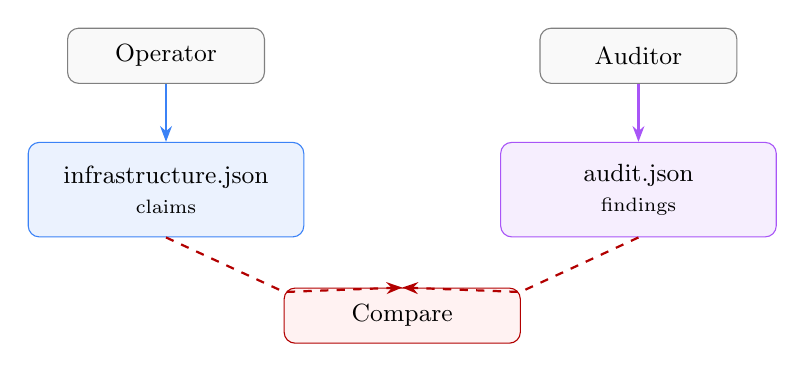
\begin{tikzpicture}[
    manifest/.style={rectangle, rounded corners, draw=#1, fill=#1!10, minimum width=3.5cm, minimum height=1.2cm, font=\small, align=center},
    actor/.style={rectangle, rounded corners, draw=gray, fill=gray!5, minimum width=2.5cm, minimum height=0.7cm, font=\small},
    arrow/.style={-{Stealth[length=2mm]}, thick},
    compare/.style={rectangle, rounded corners, draw=red!70!black, fill=red!5, minimum width=3cm, minimum height=0.7cm, font=\small}
]
\node[actor] (operator) at (0,2.5) {Operator};
\node[actor] (auditor) at (6,2.5) {Auditor};
\node[manifest=codecolor] (infra) at (0,0.8) {infrastructure.json\\{\scriptsize claims}};
\node[manifest=auditcolor] (corrig) at (6,0.8) {audit.json\\{\scriptsize findings}};
\draw[arrow, codecolor] (operator) -- (infra);
\draw[arrow, auditcolor] (auditor) -- (corrig);
\node[compare] (compare) at (3,-0.8) {Compare};
\draw[arrow, red!70!black, dashed] (infra.south) -- (1.5,-0.5) -- (compare.north);
\draw[arrow, red!70!black, dashed] (corrig.south) -- (4.5,-0.5) -- (compare.north);
\end{tikzpicture}
\caption{Adversarial Verification Architecture. Operators declare; Auditors verify. The structural gap constitutes the audit finding.}
\label{fig:manifests}
\end{figure}

\subsection{Interpretation: The Non-Authoritativeness of Determination}

A critical logic gate in this framework is the derivation of status.

\begin{claim}[Derived, Non-Authoritative Determination]
\label{claim:determination-non-authoritative}
The \texttt{determination} object in \texttt{audit.json} is a derived convenience field. It is \textbf{not authoritative}.
\end{claim}

Any value asserted in \texttt{determination} MUST be mechanically recomputed from the \texttt{tests} object by evaluators or courts. If an auditor asserts \texttt{corrigible: true} but the \texttt{tests} object contains a failure, the manifest is strictly invalid. This rule ensures that no actor (operator, auditor, or regulator) can ``declare'' a system corrigible by fiat; status exists only as the computed sum of observable structural properties.

\section{Formal Structural Model}
\label{appendix:proofs}

\paragraph{Executive Summary (Non-Technical Overview).}
This appendix formalizes two core claims of the paper using control theory as a structural model:
\begin{enumerate}[noitemsep]
    \item \textbf{Null-Feedback Instability:} If any component of the feedback path is structurally severed, the system operates as open-loop and will diverge under persistent disturbance.
    \item \textbf{Correction Velocity Inequality:} If the rate of digital error propagation exceeds the rate of institutional correction, post-hoc remedies are insufficient to prevent systemic failure.
\end{enumerate}
This formalization illustrates structural relationships between the five tests and feedback system properties. It does not claim that DPI literally behaves as a linear time-invariant system; the model is pedagogical, clarifying \textit{one half} of why partial compliance represents structural failure rather than partial success. The other half is the political-theoretic argument developed in Section~\ref{subsubsec:two-pronged}: even where partial feedback transmits \textit{some} corrective signal, partial contestation produces sham governance under a non-domination criterion. The binarity of corrigibility rests on the conjunction of the control-theoretic and political-theoretic arguments; this appendix supplies only the former.

\medskip

To formalize the assertion that ``partial corrigibility is a fatal structural failure,'' we model Digital Public Infrastructure as a standard feedback control system subject to environmental disturbance.

\subsection{Open-Loop Instability Model}

Let a DPI system state $y(t)$ (actual impact) be expected to track a reference target $r(t)$ (intended policy/rights), subject to environmental disturbance $d(t)$ (attacks, changing demographics, fraud).

The error signal (grievance) is defined as:
\begin{equation}
e(t) = r(t) - y(t)
\end{equation}

In a closed-loop system, the corrective action $u(t)$ (GOVERN) is a function of the detected error via a feedback controller $K$ (GOVERN logic) and a sensor transfer function $H$ (AUDIT/EXIT mechanism):
\begin{equation}
u(t) = K(t) \cdot H(e(t))
\end{equation}

The plant dynamics (DPI operation) are given by:
\begin{equation}
\dot{y}(t) = u(t) + d(t)
\end{equation}

\begin{proposition}[Null-Feedback Instability --- Structural Analogy]
\label{thm:null-feedback}
If any component of the feedback path is structurally broken, specifically if Sensor Transparency $H=0$ (Failed AUDIT) or Actuator Coupling $K=0$ (Failed GOVERN), the system effectively operates as Open Loop. Under Open Loop conditions with non-zero integrating disturbance $d(t)$, the error $e(t)$ diverges unboundedly.
\end{proposition}

\begin{proof}
We treat this as a structural analogy rather than a stability theorem for any specified DPI implementation; the formal apparatus illustrates the consequence of broken loop closure under generic disturbance, not the predicted dynamics of a particular system.

If tests \textbf{AUDIT} or \textbf{EXIT} fail, $H=0$.
If test \textbf{GOVERN} fails, $K=0$.
In either case, the effective corrective feedback is $u_{fb} = 0$.
The system evolution depends only on initial intent $u_{open}$ and disturbance:
\begin{equation}
y(t) = \int_0^t (u_{open}(\tau) + d(\tau)) d\tau
\end{equation}
Given that environmental variety $d(t)$ is stochastic and non-zero (Ashby's Law), and without negative feedback to compensate:
\begin{equation}
\lim_{t \to \infty} |r(t) - y(t)| \to \infty
\end{equation}
Thus, structural stability is unattainable without the closure of the feedback loop. ``Partial'' corrigibility (where $K=0$ or $H=0$) yields the same asymptotic divergence profile as fully open-loop operation.
\end{proof}

\begin{corollary}[Binarity of Corrigibility]
Corrigibility is a binary structural property, on two clauses. \textit{Mechanism clause}: if EXIT, AUDIT, or GOVERN fails, a loop-gain term vanishes, the loop opens, and systemic error cannot be structurally bounded. \textit{Verifiability clause}: if CODE or FORK fails, correction becomes unverifiable or unenforceable in extremis --- the plant is unintelligible or irreplaceable --- so corrective authority becomes discretionary rather than guaranteed. Under either clause the determination is failure.
\end{corollary}

\textit{Justification}: Each test corresponds to a necessary component of the corrective apparatus (Figure~\ref{fig:control-model}). The corollary rests on the conjunction of two independent arguments developed in Section~\ref{subsubsec:two-pronged}. \textit{Mechanism (this appendix):} from Proposition~\ref{thm:null-feedback}, since $L(s) = K(s) \cdot P(s) \cdot H(s)$, if any multiplicative term is zero the loop gain vanishes and partial compliance does not preserve closure. \textit{Legitimacy (main text):} partial contestation produces \textit{sham governance} --- accountability with non-monotonic returns where additional procedural gestures may absorb political pressure without yielding correction --- so even where partial feedback transmits some signal, the system fails the non-domination criterion (Section~\ref{sec:theory}, Normative Anchor). The mechanism argument alone yields divergence-rate claims; the legitimacy argument alone yields institutional-status claims; the conjunction yields binarity.

\begin{remark}[The Gradient Quantifier: Corrigibility at the Margin]
\label{rem:argmin}
The Corollary is evaluated at the bottom of the gradient. Proposition~\ref{thm:null-feedback} treats $H$ and $K$ as system constants. In population-scale infrastructure, they are distributions over participant position $x$ in the social hierarchy: $H(x)$ is the probability that a grievance from position $x$ generates a registered error signal, and $K(x)$ is the probability that a registered error triggers binding correction visible to $x$. Both are lowest at the least-resourced stratum --- depressed by digital literacy, language, connectivity, time, administrative precarity, and fear of retaliation.

Loop closure must hold for all participants, not on average:
\begin{equation}
\text{LoopClosed}(S) \iff \forall x \in \mathcal{X}: H(x) > 0 \;\land\; K(x) > 0
\end{equation}
The binding determination is taken at $x^* = \arg\min_x \bigl[ H(x) \cdot K(x) \bigr]$, not at the population mean. A system that closes the loop for median users while $H(x^*) = 0$ or $K(x^*) = 0$ at the margin satisfies the formal model for the comfortable majority and fails it entirely for those the framework's own evidence (Section~\ref{sec:diagnosis}) shows are most harmed by incorrigibility.

Operationally: proxy metrics and audit sampling frames must be reported as distributions. Pass/fail determination is taken at a specified lower quantile of the affected population (recommended: $p_{10}$ stratum, or the stratum documented as least-resourced in the operator's disclosure), not at the mean or aggregate rate. An audit that samples only median-resource users has not assessed whether the loop is closed; it has assessed whether the loop is closed for a particular sub-population that is structurally unlikely to include the framework's central case.
\end{remark}

\begin{figure}[htbp]
\centering
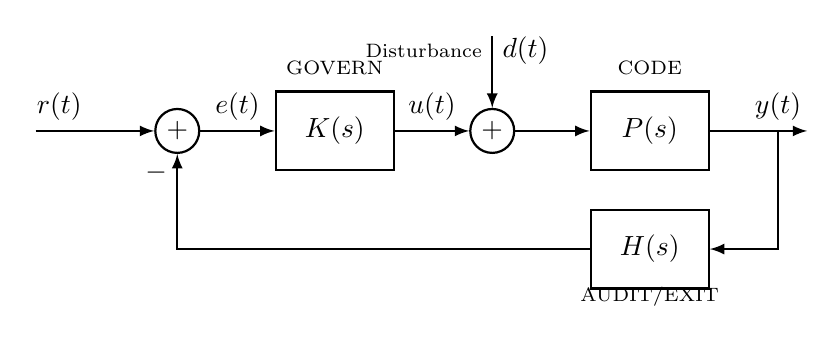
\begin{tikzpicture}[node distance=1.8cm, auto, >=latex, thick]
    % Styles
    \tikzstyle{block} = [draw, rectangle, minimum height=1cm, minimum width=1.5cm]
    \tikzstyle{sum} = [draw, circle, inner sep=2pt]
    \tikzstyle{input} = [coordinate]
    \tikzstyle{output} = [coordinate]

    % Nodes
    \node [input] (rinput) {};
    \node [sum, right of=rinput] (sum1) {$+$};
    \node [block, right of=sum1, node distance=2cm] (K) {$K(s)$};
    \node [sum, right of=K, node distance=2cm] (sum2) {$+$};
    \node [block, right of=sum2, node distance=2cm] (P) {$P(s)$};
    \node [output, right of=P, node distance=2cm] (output) {};
    \node [block, below of=P, node distance=1.5cm] (H) {$H(s)$};
    \node [input, above of=sum2, node distance=1.2cm] (disturbance) {};

    % Labels
    \node [above of=K, node distance=0.8cm] {\scriptsize GOVERN};
    \node [below of=H, node distance=0.6cm] {\scriptsize AUDIT/EXIT};
    \node [above of=P, node distance=0.8cm] {\scriptsize CODE};

    % Connections
    \draw [->] (rinput) -- node[pos=0.2] {$r(t)$} (sum1);
    \draw [->] (sum1) -- node {$e(t)$} (K);
    \draw [->] (K) -- node {$u(t)$} (sum2);
    \draw [->] (sum2) -- (P);
    \draw [->] (P) -- node [name=y, pos=0.7] {$y(t)$} (output);
    \draw [->] (y) |- (H);
    \draw [->] (H) -| node[pos=0.9, left] {$-$} (sum1);
    \draw [->] (disturbance) -- node[pos=0.2, right] {$d(t)$} node[pos=0.2, left] {\scriptsize Disturbance} (sum2);
\end{tikzpicture}
\caption{\textbf{Control-theoretic model of corrigible infrastructure.} $K(s)$: governance controller. $H(s)$: sensor/audit function. $P(s)$: plant (infrastructure). $d(t)$: environmental disturbance.}
\label{fig:control-model}
\end{figure}

The closed-loop transfer function from reference to output is:
\begin{equation}
\frac{Y(s)}{R(s)} = \frac{K(s)P(s)}{1 + K(s)P(s)H(s)}
\end{equation}

The transfer function from disturbance to output is:
\begin{equation}
\frac{Y(s)}{D(s)} = \frac{P(s)}{1 + K(s)P(s)H(s)}
\end{equation}

Corrigibility requires that each component exists and is non-degenerate:
\begin{itemize}
    \item EXIT $\Rightarrow$ $e(t) \neq 0$ observable (error signal exists)
    \item AUDIT $\Rightarrow$ $H(s) \neq 0$ (sensor functional)
    \item GOVERN $\Rightarrow$ $K(s) \neq 0$ (actuator functional)
    \item CODE $\Rightarrow$ $P(s)$ is intelligible
    \item FORK $\Rightarrow$ $P, K, H$ replaceable if convergence fails
\end{itemize}

\noindent \textbf{Active Deception as Sensor Attack.} The pathologies defined in Section~\ref{subsec:active-deception} (open-washing, safety-washing, audit theater) fundamentally corrupt the sensor function $H(s)$: they either suppress the true error signal $e(t)$ or inject artificial stability metrics, thereby blinding the controller $K(s)$ to the actual divergence $y(t) - r(t)$. In control-theoretic terms, Active Deception renders $H(s) \to 0$ not by removing the sensor, but by making its output uncorrelated with the true system state. Figure~\ref{fig:open-loop} depicts the resulting open-loop topology in which a corrupted or absent $H(s)$ severs the feedback path.

\begin{figure}[htbp]
\centering
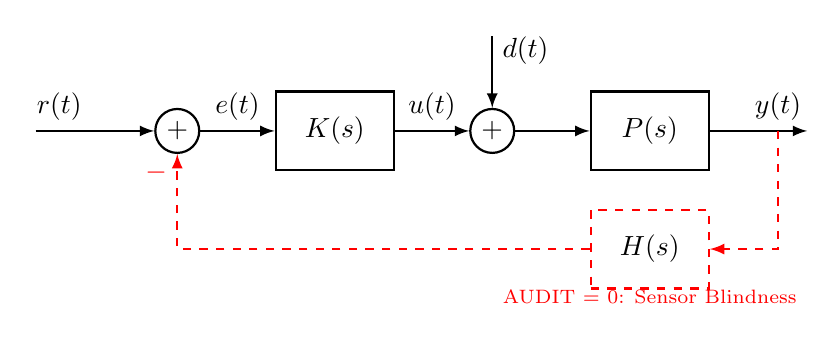
\begin{tikzpicture}[node distance=1.8cm, auto, >=latex, thick]
    \tikzstyle{block} = [draw, rectangle, minimum height=1cm, minimum width=1.5cm]
    \tikzstyle{sum} = [draw, circle, inner sep=2pt]
    \tikzstyle{input} = [coordinate]
    \tikzstyle{output} = [coordinate]

    \node [input] (rinput) {};
    \node [sum, right of=rinput] (sum1) {$+$};
    \node [block, right of=sum1, node distance=2cm] (K) {$K(s)$};
    \node [sum, right of=K, node distance=2cm] (sum2) {$+$};
    \node [block, right of=sum2, node distance=2cm] (P) {$P(s)$};
    \node [output, right of=P, node distance=2cm] (output) {};
    \node [block, below of=P, node distance=1.5cm, draw=red, dashed] (H) {$H(s)$};
    \node [input, above of=sum2, node distance=1.2cm] (disturbance) {};

    \node [below of=H, node distance=0.6cm, red] {\scriptsize AUDIT = 0: Sensor Blindness};

    \draw [->] (rinput) -- node[pos=0.2] {$r(t)$} (sum1);
    \draw [->] (sum1) -- node {$e(t)$} (K);
    \draw [->] (K) -- node {$u(t)$} (sum2);
    \draw [->] (sum2) -- (P);
    \draw [->] (P) -- node [name=y, pos=0.7] {$y(t)$} (output);
    \draw [->, dashed, red] (y) |- (H);
    \draw [->, dashed, red] (H) -| node[pos=0.9, left] {$-$} (sum1);
    \draw [->] (disturbance) -- node[pos=0.2, right] {$d(t)$} (sum2);
\end{tikzpicture}
\caption{\textbf{Open-loop failure mode.} When AUDIT fails ($H = 0$), the feedback path is severed. Equivalent failure occurs if GOVERN ($K = 0$) or EXIT ($e(t) \equiv 0$) is removed.}
\label{fig:open-loop}
\end{figure}

\subsection{The Strict Correction Velocity Inequality}

For the system to remain stable not just asymptotically but locally (preventing irreversible harm), the correction rate must dominate the error rate. We formalize this with a friction coefficient.

\begin{condition}[Strict Dynamic Stability]
\label{cond:friction}
Let $\epsilon > 0$ represent the ``friction cost'' of correction (e.g., litigation time, protest cost). A system is stable iff:
\begin{equation}
\left| \frac{d}{dt} C(t) \right| \ge \left| \frac{d}{dt} E(t) \right| + \epsilon
\end{equation}
The symmetric upper bound completes the principle stated in Section~\ref{subsec:velocity}: correction faster than it can itself be verified enables manipulated ``corrections'' to bypass review, so $|dC/dt| \le V_{\text{verify}}$, where $V_{\text{verify}}$ is the rate at which corrective actions can be independently checked. Deliberative latency is not friction to be minimized past this bound; it is the verification budget.
\end{condition}

\textbf{Implication:} Post-hoc remedies (Courts/Ombudsmen) have a linear or constant rate of operation ($\frac{dC}{dt} = k$). Digital errors propagate at exponential or high-frequency rates ($\frac{dE}{dt} \propto e^{t}$). Since for any constants there exists a time beyond which the exponential rate exceeds any linear rate --- and does so permanently --- relying on external courts guarantees eventual, unbounded accumulation of unresolved harm (Figure~\ref{fig:velocity-mismatch}). Where the execution substrate settles irreversibly, the inequality binds at a hard deadline as well as a rate: correction must reach a decision before the substrate makes it final, after which no correction velocity suffices. The correction logic must be intrinsic to the loop.

\begin{figure}[htbp]
\centering
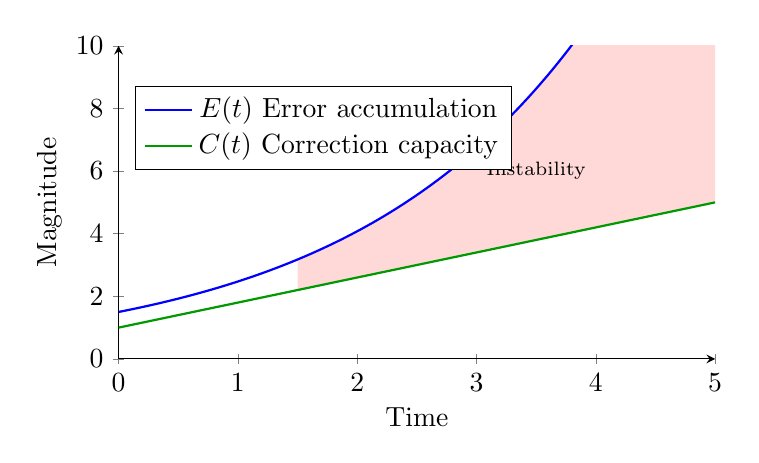
\begin{tikzpicture}[scale=0.9]
    \begin{axis}[
        xlabel={Time},
        ylabel={Magnitude},
        xmin=0, xmax=5,
        ymin=0, ymax=10,
        legend pos=north west,
        axis lines=left,
        domain=0:5,
        samples=100,
        width=10cm,
        height=6cm
    ]
    \addplot[blue, thick, name path=E] {1.5*exp(0.5*x)};
    \addlegendentry{$E(t)$ Error accumulation}
    \addplot[green!60!black, thick, name path=C] {1 + 0.8*x};
    \addlegendentry{$C(t)$ Correction capacity}
    \addplot[red!30, opacity=0.5] fill between[of=E and C, soft clip={domain=1.5:5}];
    \node at (axis cs:3.5,6) {\scriptsize Instability};
    \end{axis}
\end{tikzpicture}
\caption{\textbf{Correction velocity mismatch.} Error $E(t)$ accumulates faster than correction $C(t)$ in bureaucratic systems. The shaded region represents accumulated unresolved harm.}
\label{fig:velocity-mismatch}
\end{figure}

\subsection{Mapping to the Five Tests}

Each of the five corrigibility tests corresponds to a distinct component of the closed-loop control structure; the failure mode under each test follows directly from the role of that component (Table~\ref{tab:control-mapping}).

\begin{table}[htbp]
\centering
\caption{Mapping corrigibility tests to control-theoretic components}
\label{tab:control-mapping}
\begin{tabular}{lll}
\hline
\textbf{Test} & \textbf{Control Component} & \textbf{Failure Mode} \\
\hline
EXIT & Error Signal & Reference collapse \\
CODE & Signal Integrity & Noise indistinguishable from intent \\
AUDIT & Sensor & Blind control \\
GOVERN & Actuator & No corrective force \\
FORK & Variety Expansion & Monolithic collapse \\
\hline
\end{tabular}
\end{table}

\subsection{Measurement Procedures for Reproducibility}
\label{subsec:measurement}

To enable third-party reproduction of pass/fail determinations, each test requires specific evidence types:

\begin{table}[htbp]
\centering
\small
\caption{Evidence requirements for reproducible assessment}
\label{tab:evidence-requirements}
\begin{tabular}{@{}lp{5cm}p{5cm}@{}}
\toprule
\textbf{Test} & \textbf{Required Evidence} & \textbf{Verification Method} \\
\midrule
EXIT & (1) Legal mandate status, (2) documented alternative pathways, (3) penalty documentation & Survey of legal instruments; cost comparison with alternatives; user testimony \\
CODE & (1) Source repository URL, (2) build reproducibility proof, (3) execution path coverage & Hash verification; deterministic build; static analysis of critical paths \\
AUDIT & (1) API documentation, (2) data access agreement, (3) historical error rate publication & Attempt independent measurement; verify data freshness; compare operator vs independent findings \\
GOVERN & (1) Charter/statute URL with hash, (2) governance action log, (3) enforcement history & Legal analysis; search for overruled operator decisions; verify binding mechanism \\
FORK & (1) License text, (2) technical artifact availability, (3) resource cost estimate, (4) successful fork examples & License audit; attempt reproduction; cost modeling; historical fork survey \\
\bottomrule
\end{tabular}
\end{table}

\paragraph{Reproducibility Standard.} An assessment is reproducible if an independent auditor, given only the evidence artifacts listed above, reaches the same pass/fail determination. Disagreements must trace to (a) threshold calibration differences or (b) missing evidence, not to ambiguity in the test definitions themselves. Continuous metrics and threshold protocols are provided in Tables~\ref{tab:operational-proxies-main} and~\ref{tab:three-indicator-main} (Section~\ref{subsec:methodology}).

\subsection{Restatements of the Instability Result}

The proposition above admits several equivalent restatements that may be more familiar to readers from different traditions. None is independently load-bearing; each makes the same instability claim from a different angle (frequency domain, discrete time, cumulative rates).

\paragraph{Frequency-domain restatement.} For small perturbations around a nominal operating point, the sensitivity function $S(s) = 1 / (1 + L(s))$ with loop gain $L(s) = K(s) P(s) H(s)$ characterizes disturbance propagation. Whenever any corrigibility test fails ($K=0$, $H=0$, or the error signal is blocked), $L(s) \to 0$ and $S(s) \to 1$: disturbances pass through unattenuated. This is the same instability claim of Proposition~\ref{thm:null-feedback}, expressed in the frequency domain.

\paragraph{Discrete-time restatement.}
\label{subsec:discrete-integrator}
Consider a discrete-time scalar integrator $y_{k+1} = y_k + d_k - u_k$, where $d_k$ is a disturbance and $u_k$ is the correction. In open loop ($u_k = 0$), $y_N = y_0 + \sum_{k=0}^{N-1} d_k$, and for any non-zero mean disturbance $\mathbb{E}[d_k] = \mu > 0$ the expected state grows linearly: $\mathbb{E}[y_N] = y_0 + N\mu \to \infty$. This provides an elementary, discrete demonstration of the same divergence result.

\paragraph{Friction cost in the discrete model.} The friction coefficient $\epsilon$ from Condition~\ref{cond:friction} manifests here as a delay or reduction in the correction term. If correction requires bureaucratic processing with latency $\tau$ time steps and efficiency loss $\eta < 1$, then $u_k = \eta \cdot f(y_{k-\tau}, d_{k-\tau})$ for some feedback policy $f(\cdot)$. When $\tau > 0$ or $\eta < 1$, the effective correction rate is reduced, directly corresponding to the continuous-time friction cost $\epsilon > 0$. The stability condition $|dC/dt| \geq |dE/dt| + \epsilon$ translates to requiring the feedback policy to over-correct relative to the disturbance rate, accounting for these frictional losses.

\paragraph{Cumulative-rate restatement.} Letting $E(t)$ and $C(t)$ denote cumulative error and cumulative correction, stability requires $E(t) - C(t) < M$ for some bound $M$ and all $t > 0$, equivalently $\dot{C}(t) \geq \dot{E}(t)$ on average. When correction operates through channels with bounded throughput $\dot{C}_{\max}$ while errors grow super-linearly, a critical time $t^*$ exists beyond which correction can never catch up. This is Condition~\ref{cond:friction} restated in cumulative form.

\subsection{Functional Exit Equivalence Formalization}

An essential system $S$ satisfies FEE if compensatory architectural guarantees recreate the same effective error-signal strength that exit provides in non-essential systems.

Let:
\begin{itemize}[noitemsep]
    \item $E_{\text{exit}}^{\text{baseline}}$ = effective error-signal strength produced by real exit (non-essential case)
    \item $E_{\text{alt}}(S)$ = effective error-signal strength produced by compensatory mechanisms (essential case)
\end{itemize}

\begin{equation}
\text{FEE}(S) \iff E_{\text{alt}}(S) \geq \theta_E \cdot E_{\text{exit}}^{\text{baseline}}
\label{eq:fee}
\end{equation}

where $\theta_E$ is a policy calibration constant (recommended range: $0.8$--$1.0$).

\paragraph{Operationalizing $E$.} The error-signal strength $E$ can be operationalized as a weighted sum:

\begin{equation}
E = \alpha_1 \cdot \text{effective\_loss} + \alpha_2 \cdot \text{probability\_of\_departure} + \alpha_3 \cdot \text{velocity\_of\_response} + \alpha_4 \cdot \text{legal\_remedy\_speed}
\label{eq:error-signal}
\end{equation}

where the weights $\alpha_i$ are calibrated via pilot audits. All variables are operationalized such that higher values indicate greater corrective pressure on the operator.

\subsection{Switching Cost Formalization}

The practical barrier to exit and fork is operationalized through a \textbf{switching cost} scalar:

\begin{equation}
\sigma(S \to S') = c_{\text{data}} + c_{\text{downtime}} + c_{\text{reprovisioning}} + c_{\text{network}} + c_{\text{legal}}
\label{eq:switching-cost}
\end{equation}

where each component is normalized to $[0,1]$:
\begin{itemize}[noitemsep]
    \item $c_{\text{data}}$: cost of exporting and reformatting user data
    \item $c_{\text{downtime}}$: service interruption during transition
    \item $c_{\text{reprovisioning}}$: re-establishing credentials and trust relationships
    \item $c_{\text{network}}$: loss of social connections and network effects
    \item $c_{\text{legal}}$: regulatory friction and contractual barriers
\end{itemize}

\paragraph{Portability Threshold.} EXIT and FORK functionally fail when switching cost to all plausible alternatives exceeds a policy threshold:

\begin{equation}
\min_{S' \in \mathcal{A}} \sigma(S \to S') > \Sigma^* \implies \text{EXIT/FORK fail}
\label{eq:portability-threshold}
\end{equation}

where $\mathcal{A}$ is the set of available alternatives and $\Sigma^*$ is a calibrated threshold on the normalized $[0,5]$ scale of $\sigma$ (e.g., $\Sigma^* = 2.0$). Practical anchors --- switching costs exceeding $0.2$ of annual disposable income, or $30$ days' service disruption --- calibrate the \textit{individual} components $c_i$ to their maximal value of $1$; they are normalization anchors, not alternative values of $\Sigma^*$ itself.

\paragraph{Illustrative Application.} Aadhaar exhibits $\sigma \approx 4.8$ (near-maximal) because $c_{\text{data}} = 1$ (no export), $c_{\text{downtime}} = 1$ (total service denial), and $c_{\text{legal}} = 1$ (mandate forecloses alternatives). UPI retains $\sigma \approx 1.0$--$1.5$ because cash and cards remain legal. With $\Sigma^* = 2.0$, Aadhaar categorically fails on the switching-cost criterion, while UPI does not fail on that criterion --- though UPI still fails FORK on the constructed-barrier dimension (Section~\ref{sec:tests}: NPCI's regulatory monopoly), since $\sigma < \Sigma^*$ licenses no pass on its own (Equation~\ref{eq:portability-threshold} is a one-way implication).

\subsection{Summary of Formal Extensions}

\begin{enumerate}
    \item Linearized restatement ties removal of $H$, $K$, or EXIT to vanishing loop gain $L(s)$, exposing unstable process modes.
    \item Discrete integrator supplies an elementary divergence demonstration and absorbs Condition~\ref{cond:friction} via the $(\eta, \tau)$ parameters.
    \item Correction velocity is formalized via Condition~\ref{cond:friction} and its cumulative-rate restatement.
    \item FEE formalization (eq.~\ref{eq:fee}) operationalizes the principle of essential-services compensation; weights $\alpha_i$ are calibrated externally.
    \item Switching-cost formalization (eq.~\ref{eq:switching-cost}, eq.~\ref{eq:portability-threshold}) operationalizes EXIT/FORK failure thresholds.
\end{enumerate}

\section{Neutrality Compression Under Centralized Enforcement}
\label{appendix:neutrality}

This appendix provides the formal proof supporting Proposition~\ref{prop:trilemma} (Topology-Dependent Tension).

\subsection{Definitions}

Let:
\begin{itemize}[noitemsep]
    \item $Sc$ = Scale (population-level integration)
    \item $V_{\text{env}}(Sc)$ = Environmental variety (heterogeneity of governed interactions)
    \item $V_{\text{gov}}(Sc)$ = Governance corrective variety
\end{itemize}

We assume:
\begin{enumerate}[noitemsep]
    \item $V_{\text{env}}(Sc)$ is non-decreasing in $Sc$ (Ashby's Law: environmental complexity grows with population scale)
    \item Under centralized enforcement, governance growth is institutionally bounded (bureaucratic capacity constraints)
\end{enumerate}

Formally:
\begin{equation}
V_{\text{gov}}(Sc) = O(Sc^{\alpha}), \quad \alpha < 1
\end{equation}
This states that governance corrective capacity grows sublinearly under centralized topology. No specific functional form (logarithmic, square root, etc.) is required. The sublinear constraint reflects institutional reality: adding staff, building appeal mechanisms, and processing edge cases cannot scale linearly with population without structural reform.

\subsection{Neutrality Condition}

Neutrality does not require full dominance of environmental variety. It requires sufficient corrective bandwidth to prevent systematic routing bias.

Define:
\begin{equation}
V_{\text{gov}} \geq \theta \cdot V_{\text{env}}
\end{equation}
Where $\theta \in (0,1]$ is a stability sufficiency constant.

\textbf{Neutrality degradation risk} emerges when:
\begin{equation}
V_{\text{gov}} < \theta \cdot V_{\text{env}}
\end{equation}
This avoids equating neutrality with perfect stability.

\subsection{Proposition (Formal Statement)}

Under centralized enforcement topology, there exists a scale threshold $Sc^*$ beyond which neutrality is at risk unless governance growth becomes at least linear in scale.

\subsection{Proof}

Assume environmental variety grows at least linearly with scale:
\begin{equation}
V_{\text{env}}(Sc) = \Omega(Sc)
\end{equation}

Under centralized enforcement:
\begin{equation}
V_{\text{gov}}(Sc) = O(Sc^{\alpha}), \quad \alpha < 1
\end{equation}

Therefore:
\begin{equation}
\frac{V_{\text{gov}}(Sc)}{V_{\text{env}}(Sc)} \to 0 \quad \text{as} \quad Sc \to \infty
\end{equation}

Thus there exists $Sc^*$ such that:
\begin{equation}
V_{\text{gov}}(Sc^*) < \theta \cdot V_{\text{env}}(Sc^*)
\end{equation}

The neutrality condition is violated. \qed

\subsection{Governance Automation Objection}

One may argue that governance capacity scales linearly through automated monitoring. However:

If governance automation is implemented within the same centralized topology, then:
\begin{itemize}[noitemsep]
    \item The automation itself requires governance oversight
    \item External corrective independence does not increase proportionally
    \item Appeal mechanisms remain institutionally bounded
\end{itemize}

Thus governance automation does not automatically imply:
\begin{equation}
V_{\text{gov}}(Sc) = \Theta(Sc)
\end{equation}
unless corrective mechanisms are externally independent and structurally distributed.

This preserves the proposition.

\subsection{Falsifiability Clause}

The theory would be falsified if a centralized sovereign DPI:
\begin{enumerate}[noitemsep]
    \item Achieves population-scale deployment
    \item Maintains governance growth $V_{\text{gov}}(Sc) = \Theta(Sc)$
    \item Sustains structural neutrality under high scale
\end{enumerate}
\textit{without} federated or multi-operator architecture.

Such a system would contradict the sublinear governance constraint. This condition is empirically testable.

\subsection{Interpretation}

The result does not assert:
\begin{itemize}[noitemsep]
    \item That scale is harmful
    \item That sovereignty is undesirable
    \item That neutrality is impossible
\end{itemize}

It asserts:
\begin{itemize}[noitemsep]
    \item Under centralized enforcement topology, governance corrective capacity must scale at least linearly with environmental complexity to preserve neutrality.
    \item Sublinear governance growth is a structural prediction of centralized architecture; neutrality degradation risk follows mathematically.
\end{itemize}

Figure~\ref{fig:variety-compression} visualizes the compression: as scale rises, environmental variety grows linearly while centralized governance variety grows at most sublinearly, so the neutrality-sufficiency threshold $\theta \cdot V_{\text{env}}$ is crossed at some scale $Sc^*$.

\begin{figure}[htbp]
\centering
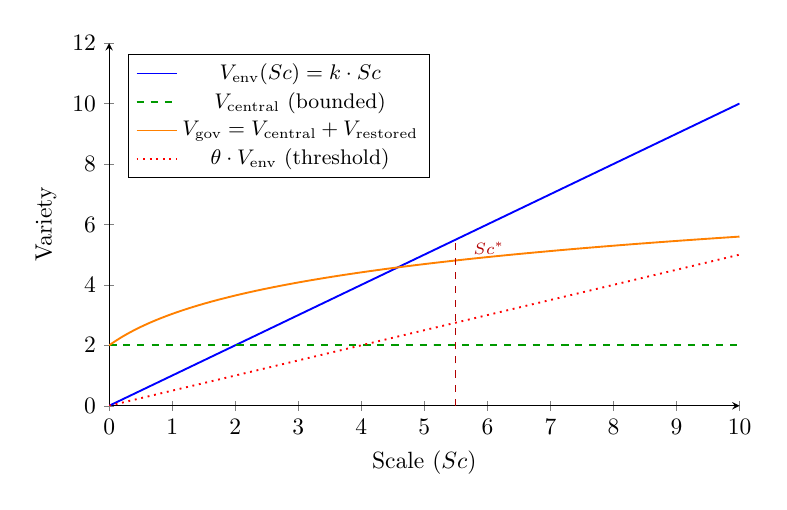
\begin{tikzpicture}[scale=0.85]
    \begin{axis}[
        xlabel={Scale ($Sc$)},
        ylabel={Variety},
        xmin=0, xmax=10,
        ymin=0, ymax=12,
        legend pos=north west,
        axis lines=left,
        domain=0:10,
        samples=100,
        width=11cm,
        height=7cm,
        legend style={font=\small}
    ]
    % Environmental variety (linear)
    \addplot[blue, thick] {x};
    \addlegendentry{$V_{\text{env}}(Sc) = k \cdot Sc$}

    % Centralized governance (constant)
    \addplot[green!60!black, thick, dashed] {2};
    \addlegendentry{$V_{\text{central}}$ (bounded)}

    % Restored variety (logarithmic growth)
    \addplot[orange, thick] {2 + 1.5*ln(x+1)};
    \addlegendentry{$V_{\text{gov}} = V_{\text{central}} + V_{\text{restored}}$}

    % Mark critical threshold
    \node[font=\scriptsize, text=red!70!black, anchor=west] at (axis cs:5.65,5.2) {$Sc^*$};
    \draw[red!70!black, dashed, thin] (axis cs:5.5,0) -- (axis cs:5.5,5.5);

    % Neutrality threshold line
    \addplot[red, thick, dotted] {0.5*x};
    \addlegendentry{$\theta \cdot V_{\text{env}}$ (threshold)}
    \end{axis}
\end{tikzpicture}
\caption{\textbf{Governance Variety Compression Under Scale.} As scale increases, environmental variety grows linearly. Under centralized enforcement, governance variety grows sublinearly (logarithmic here). Neutrality degradation risk emerges when governance variety falls below the threshold $\theta \cdot V_{\text{env}}$ (at $Sc^*$).}
\label{fig:variety-compression}
\end{figure}

\section{Verification and Enforcement Rules}
\label{appendix:rules}

To distinguish constitutive governance from performative compliance, the framework states evidentiary rules for who may speak with binding authority and whose audit verdicts count as truth. These rules close the GOVERN and AUDIT loops: without them, the operator's affidavit would float free of the auditor's finding, and the corrective channel would collapse back into narrative.

\subsection{Normative Rules}

\paragraph{Rule A.9: Operational Definition of Binding Authority}
To satisfy the GOVERN test, any escalation path claimed as ``binding'' in the Manifest MUST include:
\begin{enumerate*}[label=(\roman*)]
    \item a resolvable reference to the statute or charter (\texttt{binding\_proof\_url}),
    \item a cryptographic hash of that instrument to prevent silent amendment, and
    \item historical evidence of enforcement against the operator.
\end{enumerate*}
Assertions of authority that rely on post-execution bureaucratic discretion (e.g., ombudsmen, ``feedback forms'') do not satisfy this rule and must be marked \texttt{false}. This rule is what disqualifies advisory bodies from constituting governance, and is the operational test invoked when the main text concludes that systems such as Aadhaar fail GOVERN.

\paragraph{Rule A.10: Chain of Custody}
Auditor manifests must be canonically serialized (RFC 8785), hashed (SHA-256), and signed (Ed25519) using a valid W3C Decentralized Identifier. Unsigned assessments are treated as schema-invalid. This creates a permanent, falsifiable record of who certified a system, and is what makes an audit verdict independently checkable rather than a narrative claim.

\paragraph{Rule A.11: Auditor Data Duties}
The AUDIT guarantee (``no one can prevent auditing,'' Section~\ref{sec:tests}) does not imply unlimited data access by auditors. Audit access must be purpose-bound: auditors access minimized, purpose-specific views of system behavior --- population-level aggregates, stratified error rates, sampled records under a defined privacy budget, or replay against pseudonymized logs with subject receipts (see the Subject Receipt Requirement in the companion paper~\citep{aravind2026epi}) as the ground-truth check. Auditor manifests must declare the data accessed, the purpose, and the retention and deletion schedule for any individual-level records obtained; this declaration is itself governed by Rule~A.10 and is auditable. Violations --- data accessed beyond stated purpose, retained past the declared window, or shared with parties outside the audit engagement --- revoke the auditor's DID standing. ``No one can prevent auditing'' and ``no one can strip-mine the governed'' are not in tension; they are the two-sided requirement of the AUDIT test: permissionless access to the operator's behavior, purpose-bounded access to the governed's data. Any audit regime that satisfies the first condition while ignoring the second has extended legibility downward to the very population the test exists to protect, reproducing the asymmetric-observability failure the AUDIT test exists to correct (Section~\ref{sec:tests}).

\subsection{Tiered Identity Assurance Model}

To prevent ``identity washing'', where operators use ephemeral keys to rubber-stamp their own systems, the framework employs a tiered assurance model. Verification dashboards should weigh assessments accordingly:

\begin{enumerate}
    \item \textbf{Tier 1: Self-Attested (\texttt{did:key}):} Ephemeral identity. Suitable for whistleblowers, individual researchers, or rapid-response checks. \textit{Status: informational.}
    \item \textbf{Tier 2: Domain-Verified (\texttt{did:web}):} Identity cryptographically bound to a specific DNS domain (e.g., \texttt{did:web:eff.org}). Attribution to known civil society actors. \textit{Status: verified.}
    \item \textbf{Tier 3: Institution-Verified:} Identity anchored in transparency logs or institutional trust registries. \textit{Status: regulatory standing.}
\end{enumerate}
This tiering is what allows the AUDIT test to distinguish credible independent verification from operator self-attestation; full schema encodings of the tiers, together with the DID resolution and canonicalization details, are maintained in the schema repository (\url{https://github.com/anivar/corrigibility-schema}).

\section{Anticipated Objections and Responses}
\label{appendix:objections}

This appendix addresses the strongest objections to the framework, organized by the discipline from which they originate.

\subsection{Control Theory Objections}

\paragraph{Objection 1: Binary model ignores continuous feedback dynamics.}
``Real control systems have continuous loop gain. Partial observability and partial actuation still provide some regulation. Your binary pass/fail ignores systems that are 'mostly corrigible.'''

\textbf{Response:} The objection conflates physical description with normative threshold. We do not dispute that real systems exhibit continuous variation in feedback quality. The binary model is a \textit{legitimacy threshold}, not a physical claim (Section~\ref{sec:discussion}). A feedback loop with 50\% sensor accuracy transmits some signal; this does not mean the system deserves public trust. The determination function $D$ (Section~\ref{subsec:methodology}) makes explicit that continuous inputs feed a binary output. The threshold is where we draw the line for public legitimacy, separable from the physics.

\paragraph{Objection 2: Where is the Lyapunov stability proof?}
``You claim systems diverge without feedback. Show the Lyapunov function. Without rigorous stability analysis, this is hand-waving.''

\textbf{Response:} Appendix~\ref{appendix:proofs} provides the formal treatment. Proposition~\ref{thm:null-feedback} (Null-Feedback Instability --- Structural Analogy) shows that when $H=0$ or $K=0$, the system operates open-loop and diverges under non-zero disturbance. The discrete integrator example (Section~\ref{subsec:discrete-integrator}) provides an elementary proof: $y_N = y_0 + \sum d_k \to \infty$ for any non-zero mean disturbance. A full Lyapunov treatment would require specifying the state space for a particular DPI implementation; the framework operates at the architectural level, where the key insight (that open loops diverge) is mathematically trivial.

\subsection{Political Science Objections}

\paragraph{Objection 3: You ignore legitimate state interests.}
``Governments have valid reasons for mandatory systems: national security, public health, anti-fraud. Your framework would prohibit pandemic contact tracing.''

\textbf{Response:} The framework does not prohibit mandatory systems; it diagnoses their structural properties. Emergency necessity explains but does not justify incorrigibility (Corollary to Proposition~\ref{prop:essentiality}). A pandemic contact-tracing system can still satisfy CODE (open source), AUDIT (independent testing), GOVERN (binding privacy constraints), and FORK (interoperable protocol). Only EXIT is constrained by mandatory participation. The question is whether the other four tests pass, not whether mandates are ever legitimate. Section~\ref{sec:discussion} explicitly notes that corrigibility is compatible with strict, non-negotiable rules.

\paragraph{Objection 4: The Essentiality-Corrigibility Tension proves your framework is useless.}
``You prove essential services can never be fully corrigible. This makes your framework irrelevant for the systems that matter most: identity, payments, healthcare.''

\textbf{Response:} The proposition identifies a structural constraint, not a reason to abandon analysis. The architectural responses (Section~\ref{subsubsec:arch-responses}) show two paths: protected alternatives (guarantee non-digital equivalents) or federated implementation (no single provider essential). X-Road demonstrates 4/5 at population scale. The finding that fully corrigible essential services require architectural innovation is the framework's central contribution. Diagnosing why current systems fail is prerequisite to designing better ones.

\subsection{Empirical Objections}

\paragraph{Objection 5: Your pass/fail determinations are subjective.}
``Two auditors could reach different conclusions. Without precise, reproducible metrics, this is opinion dressed as science.''

\textbf{Response:} Section~\ref{subsec:measurement} specifies evidence requirements for each test. Table~\ref{tab:evidence-requirements} lists required artifacts and verification methods. The reproducibility standard states: an assessment is reproducible if an independent auditor, given only the evidence artifacts, reaches the same determination. Disagreements must trace to threshold calibration or missing evidence, not definition ambiguity. Rule~A.10 (Appendix~\ref{appendix:rules}) binds every audit verdict to a canonically signed manifest, making disagreements traceable rather than narrative; the JSON schemas in the schema repository encode the full field set across all five tests. Future work includes inter-rater reliability studies.

\subsection{Summary}

The framework withstands scrutiny from control theory (binary is threshold, not physics), political science (mandates can coexist with corrigibility on other dimensions), and empirical methodology (reproducible metrics exist). The strongest residual objection (network effects making FORK practically impossible even when legally permitted) is acknowledged in Limitations and proposed for formal treatment in Future Work.

\section{Glossary of Key Terms}
\label{appendix:glossary}

The glossary below is shared verbatim with the companion paper~\citep{aravind2026epi} so that terminology is identical across the pair.

% Shared glossary for DPI and EPI papers.
% Populated during the v3 revision (see CHANGELOG.md and the revision plan).
%
% Usage from each paper's main.tex:
%   % Shared glossary for DPI and EPI papers.
% Populated during the v3 revision (see CHANGELOG.md and the revision plan).
%
% Usage from each paper's main.tex:
%   % Shared glossary for DPI and EPI papers.
% Populated during the v3 revision (see CHANGELOG.md and the revision plan).
%
% Usage from each paper's main.tex:
%   \input{../shared/glossary}




% ============================================
% REFERENCES (at end, per academic standard)
% ============================================
\bibliographystyle{plainnat}
\bibliography{../shared/refs}

\end{document}
